The CP-violating asymmetries can arise due to both couplings from BSM processes and detector and reconstruction effects.
The previous study at \oldTeV used background-enriched data to study the detector bias~\cite{CPVtop:CMSresult}.
The precision in the modeling of the resulting CP-violating asymmetries caused by detector and reconstruction effects may be improved by studying signal events, and therefore an event-mixing method is used to evaluate the possible bias resulting in a nonzero value of \Acpprime.
The method using background-enriched data is also introduced here along with the event-mixing method.

\subsection{Background-enriched method}
Based on the assumption of zero asymmetry in the background events, a sample of background-enriched data events can be used to estimate the detector bias.
This sample is selected by rejecting events with b-tagged jets and is expected to be dominated by background events.
It contains a sufficiently large number of events to perform statistically significant cross checks.
However, the fraction of \ttbar event is up to about $8\%$ in this sample, which may contaminate the measured results.
Secondly, the kinematics of backgrounds may differ from top pair events, and assumption of no asymmetry in background process has to be introduced.
Therefore, in this analysis, we determine to measure detector and reconstruction bias using \ttbar events.
We believe there is no better control sample than \ttbar itself, and the statistics is much higher as well.

\subsection{Event-mixing method}
The event-mixing method is aimed to eliminate the asymmetries from new physics in the sample, and then the asymmetries coming from detector and reconstruction effects can be directly measured. 
This method is performed by mixing the four-momentum information of the \PQb-tagged jet from the hadronically decaying top quark and the highest \PT light-flavor jet among the events.
A total of 1000 mixed data sets are produced by applying the event-mixing method to the data in the signal events to eliminate possible effects from any BSM coupling.
For the $i^{\text{th}}$ mixed data set, the corresponding four-momentum information of the $j^{\text{th}}$ event is passed circularly to the $(j+i)^{\text{th}}$ event.
The resulting sets of asymmetries are independent of the physical processes involved in the signal and background events and represent only the bias from the detector and reconstruction effects.
Separate measurements are performed for each CP observable, year of data taking, and lepton flavor.
The resulting mean values of \Acpprime are presented in Table~\ref{tab:detector_bias} and show no statistically significant detector or reconstruction bias for either lepton flavor.

The correlation between different mixed samples has been studied with parton-level SM simulated \ttbar samples using \MADGRAPH.
A total of 1001 sets of data with 200k events are produced.
The event-mixing method is applied to the first set of data to produce 1000 sets of mixed samples.
The resulting \Acpprime distribution of the mixed samples and the remaining 1000 sets of data are displayed in Fig.~\ref{fig:correlation_study}.
The results show no obvious correlation between those distribution and thus the correlation between mixed samples is neglected in the following process.

This method is tested with \ttbar events with artificial \Acpprime and \ttbar events with intrinsic detector bias.
The \ttbar events with artificial \Acpprime can be produced by randomly picking up $10\%$ more events with positive \Acp in SM simulated \ttbar sample at generator level.
The results are presented in Fig.~\ref{fig:artificial_acp} with around $2$ to $4\%$ artificial \Acpprime.
The resulting mean values of \Acpprime after applying the event-mixing method to \ttbar events with artificial \Acpprime are presented in Figs.~\ref{fig:16_exchanging_simulation_acp},~\ref{fig:17_exchanging_simulation_acp},~\ref{fig:18_exchanging_simulation_acp}.
The results show no statistically significant asymmetries for either lepton flavor.
The \ttbar events with intrinsic detector bias is produced by lowering the detector resolution in SM simulated \ttbar samples.
The values of $\theta$ and $\phi$ are assigned to the same value, for example, the $\theta$ and $\phi$ of b-tagging jets are assigned to $0.5\pi$ and $0.8\pi$ if their original angle is between $0.5\pi - 0.8\pi$ and $0 - 0.67\pi$, respectively.
The test is performed with the least sensitive observable \Otwelve, and the results in Fig~\ref{fig:closure_test_acp} show that the event-mixing method can retain the intrinsic bias.

\subsection{Asymmetries in simulated samples}
The expected values of \Acpprime are supposed to be zero in SM simulated \ttbar and background events.
However, the \Acpprime might be biased due to the imperfection during the simulation process.

The \Acpprime value for SM simulated \ttbar are shown with only statistical uncertainties in Fig~\ref{fig:simulated_signal_acp}, and the \Acpprime values of simulated backgrounds are shown in Fig~\ref{fig:simulated_background_acp}.
Both results show no significant bias  within two standard deviation after combining both the electron and muon channel which is consistent with the prediction from standard model.

\begin{figure}
    \centering
    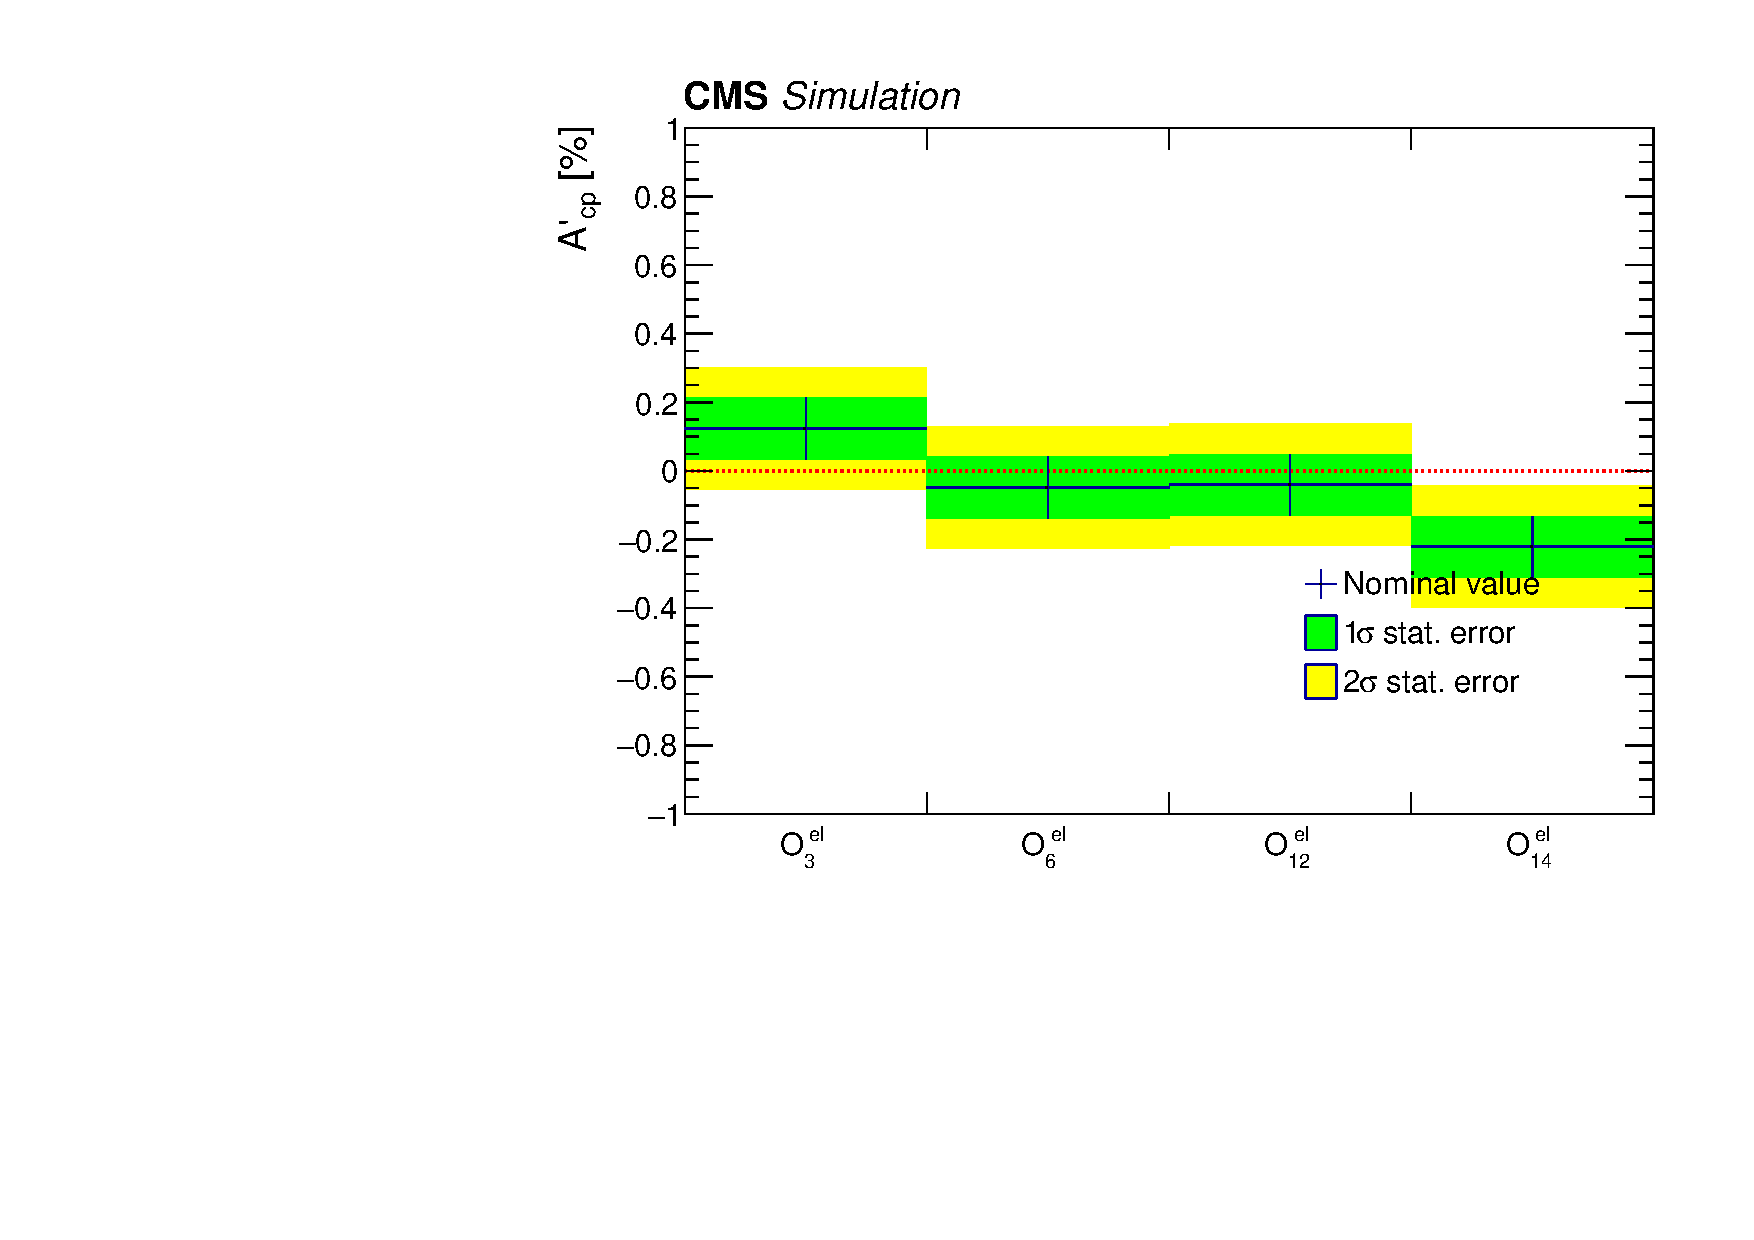
\includegraphics[width=0.45\textwidth]{figure/SimAcp_16_el_ttbar_chi2_20_opt_150.pdf}
    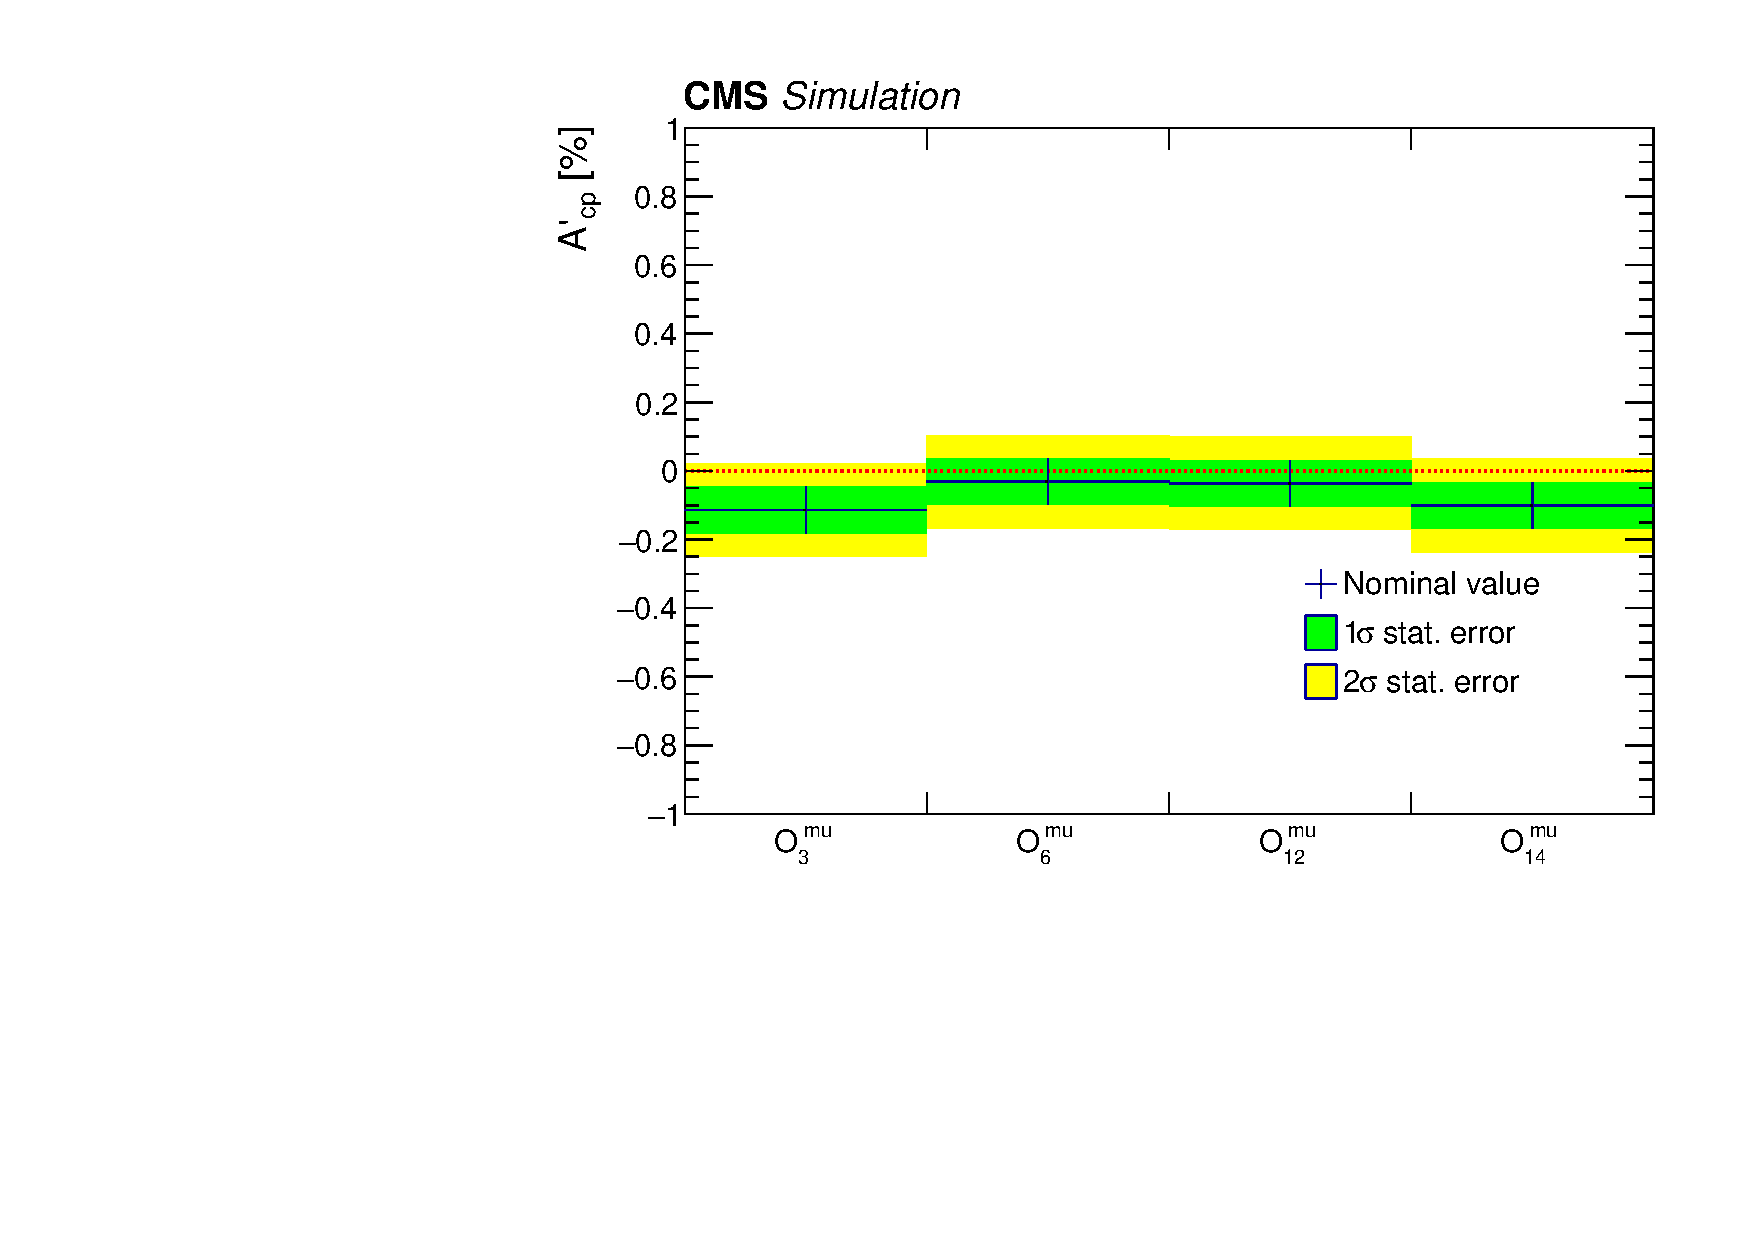
\includegraphics[width=0.45\textwidth]{figure/SimAcp_16_mu_ttbar_chi2_20_opt_150.pdf}
    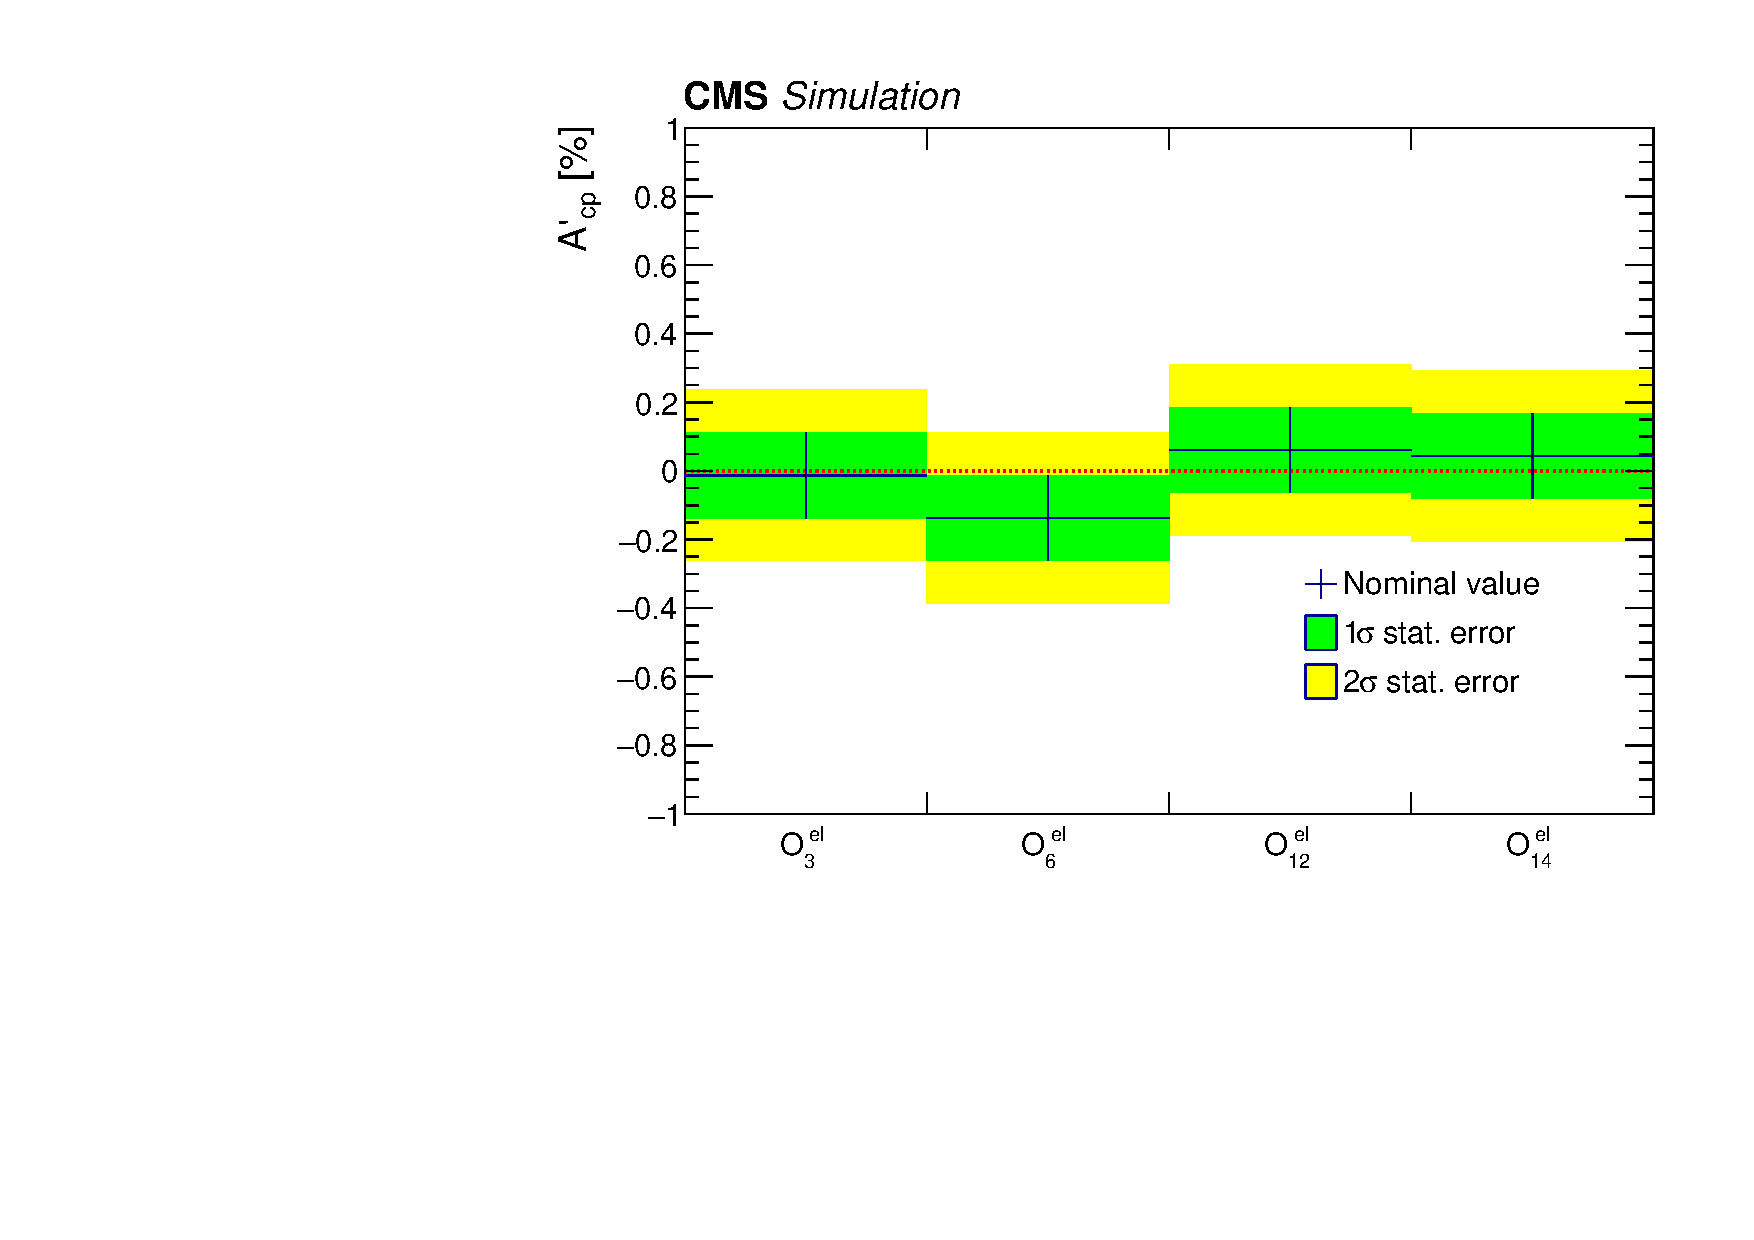
\includegraphics[width=0.45\textwidth]{figure/SimAcp_17_el_ttbar_chi2_20_opt_150.pdf}
    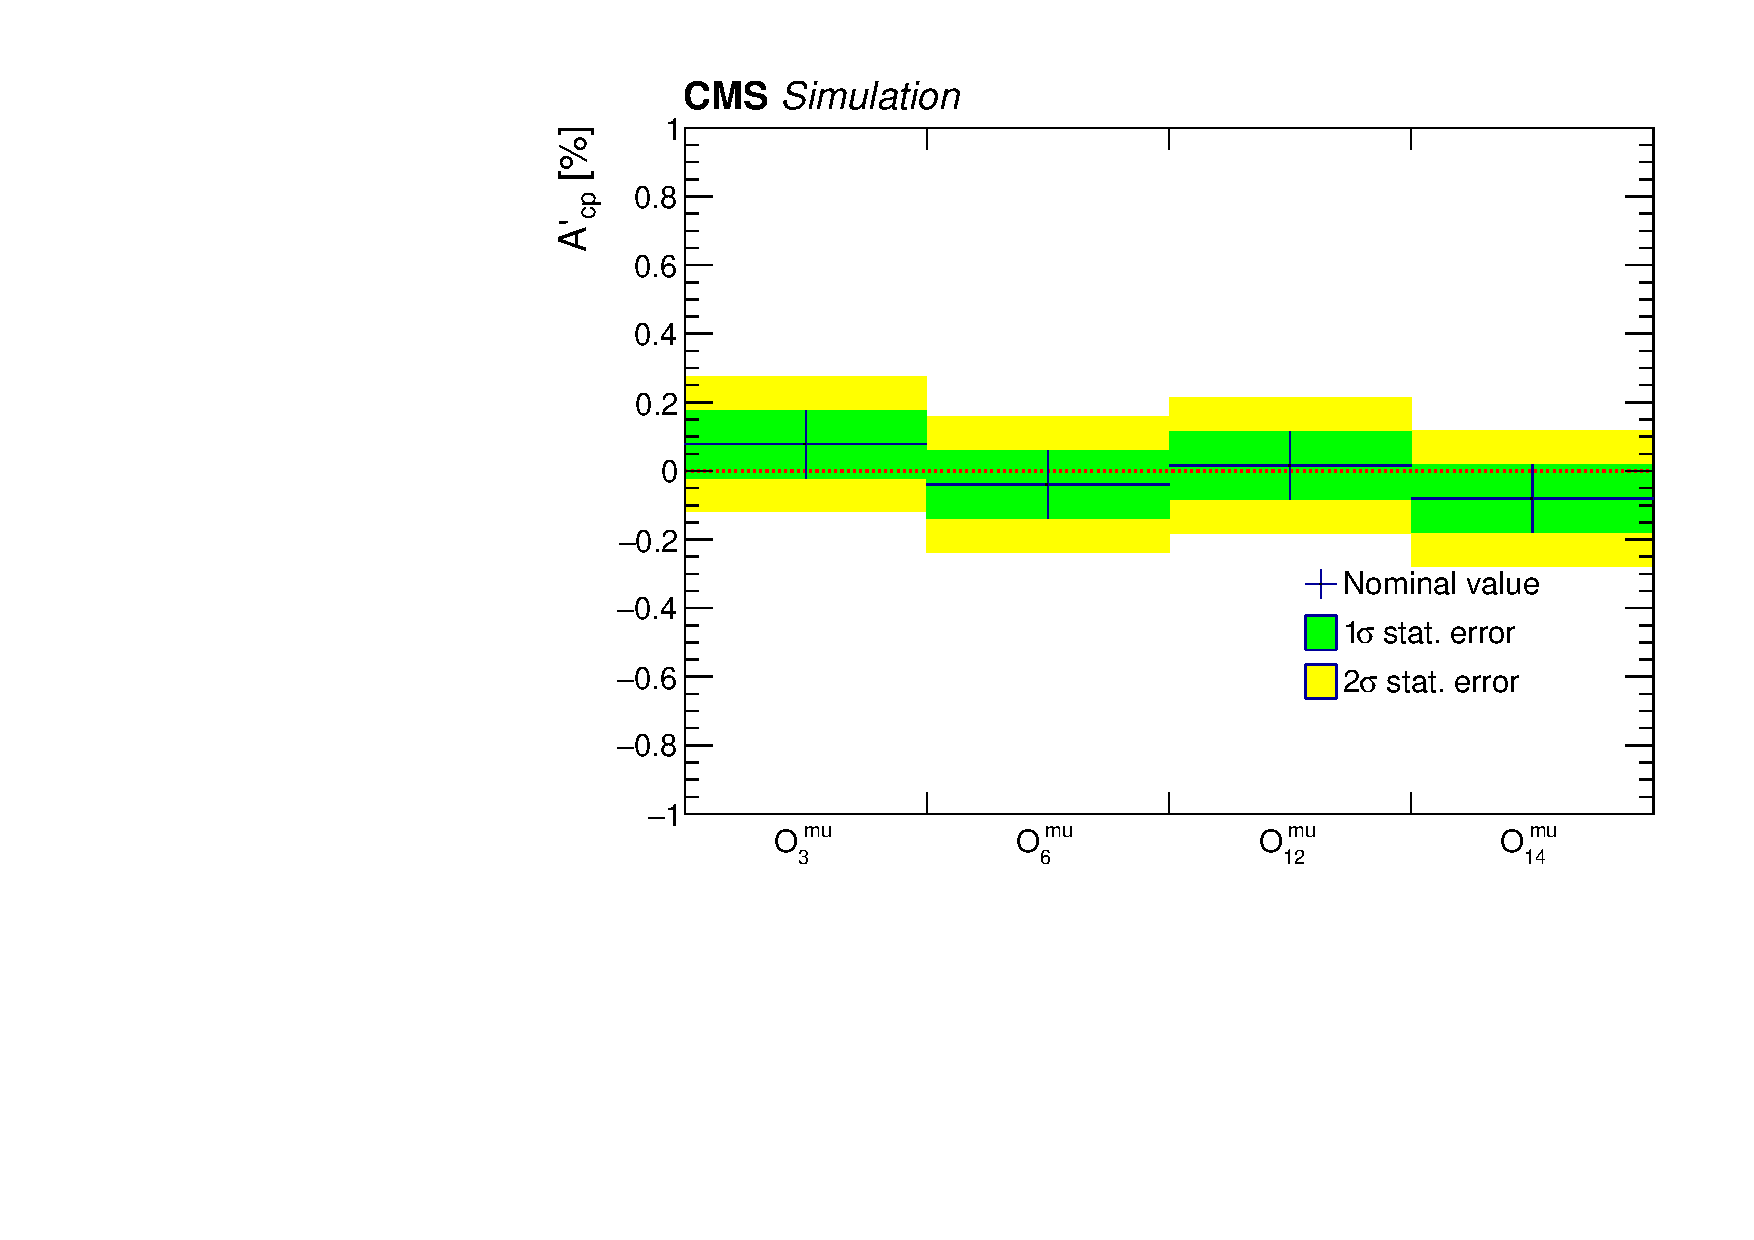
\includegraphics[width=0.45\textwidth]{figure/SimAcp_17_mu_ttbar_chi2_20_opt_150.pdf}
    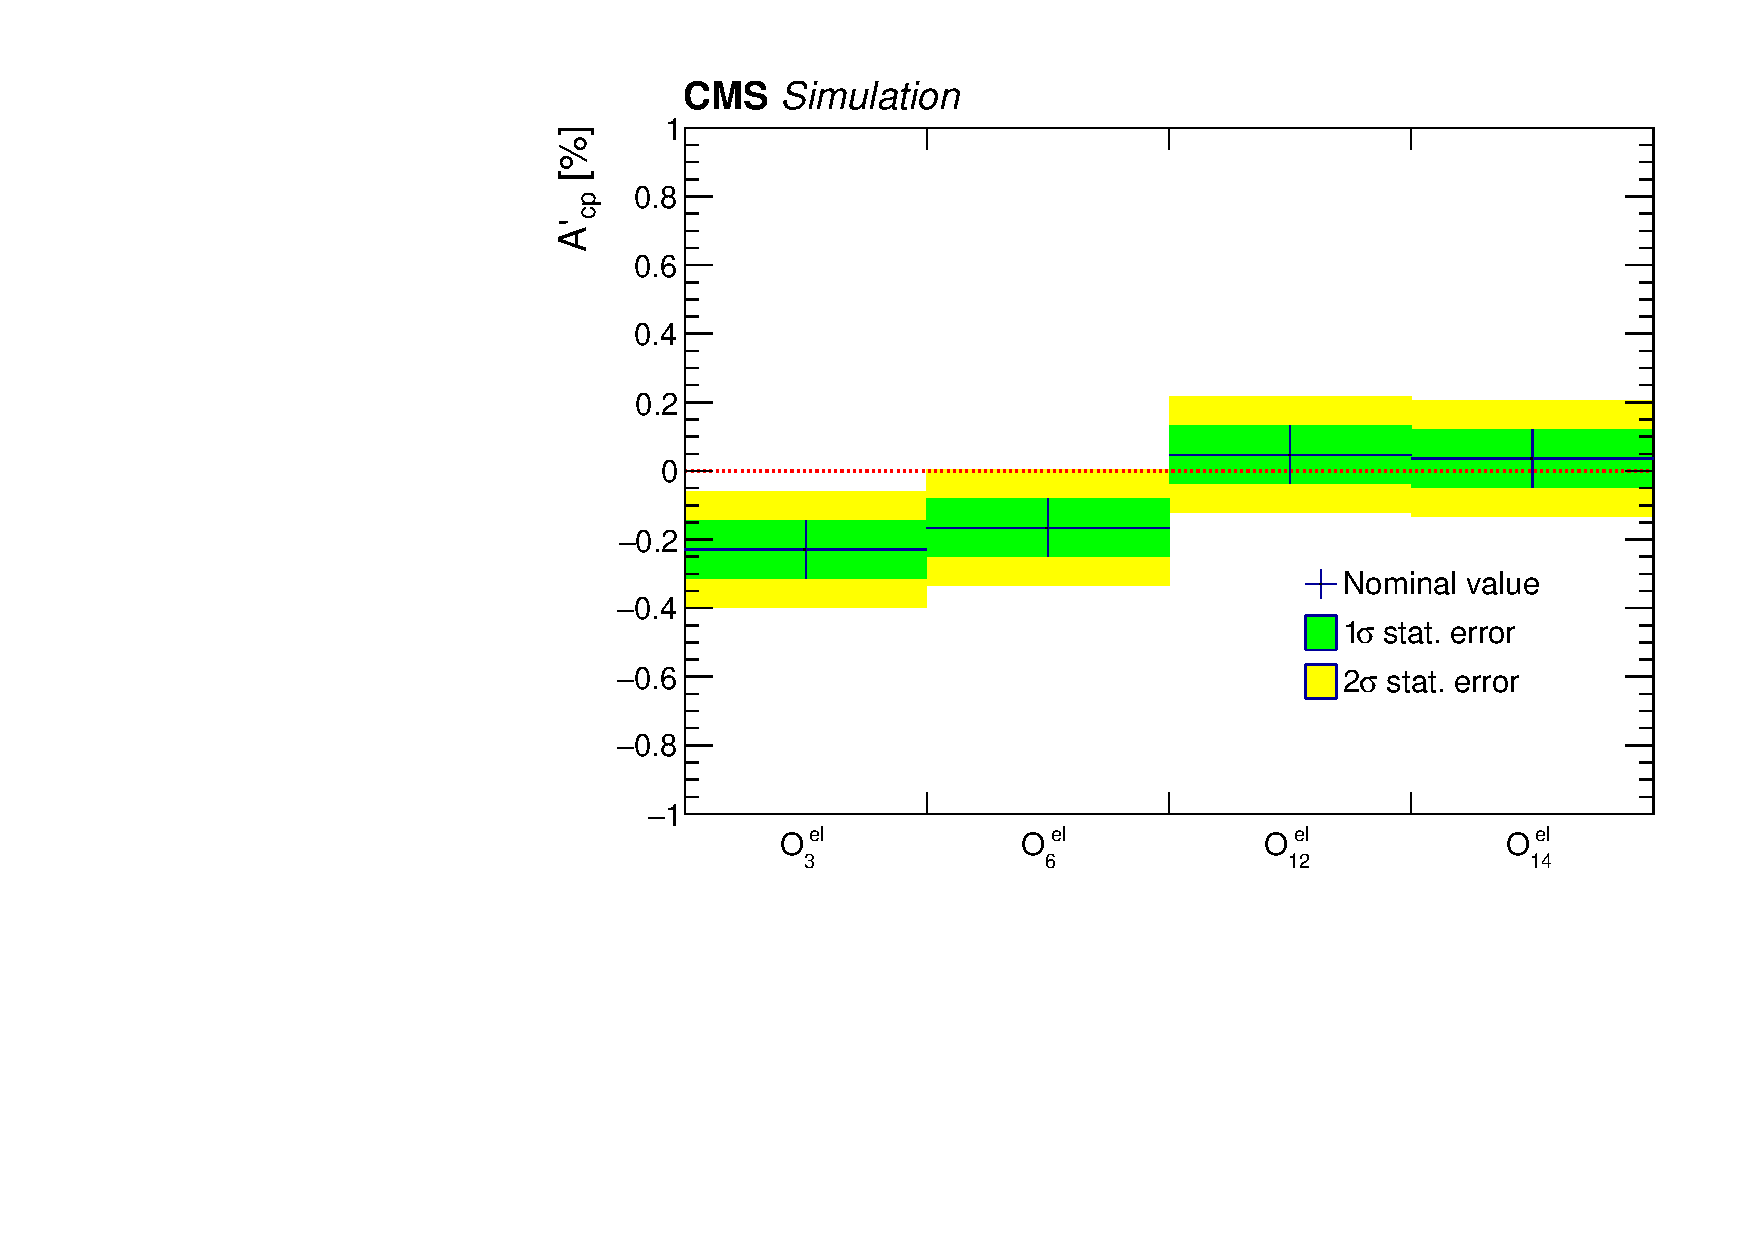
\includegraphics[width=0.45\textwidth]{figure/SimAcp_18_el_ttbar_chi2_20_opt_150.pdf}
    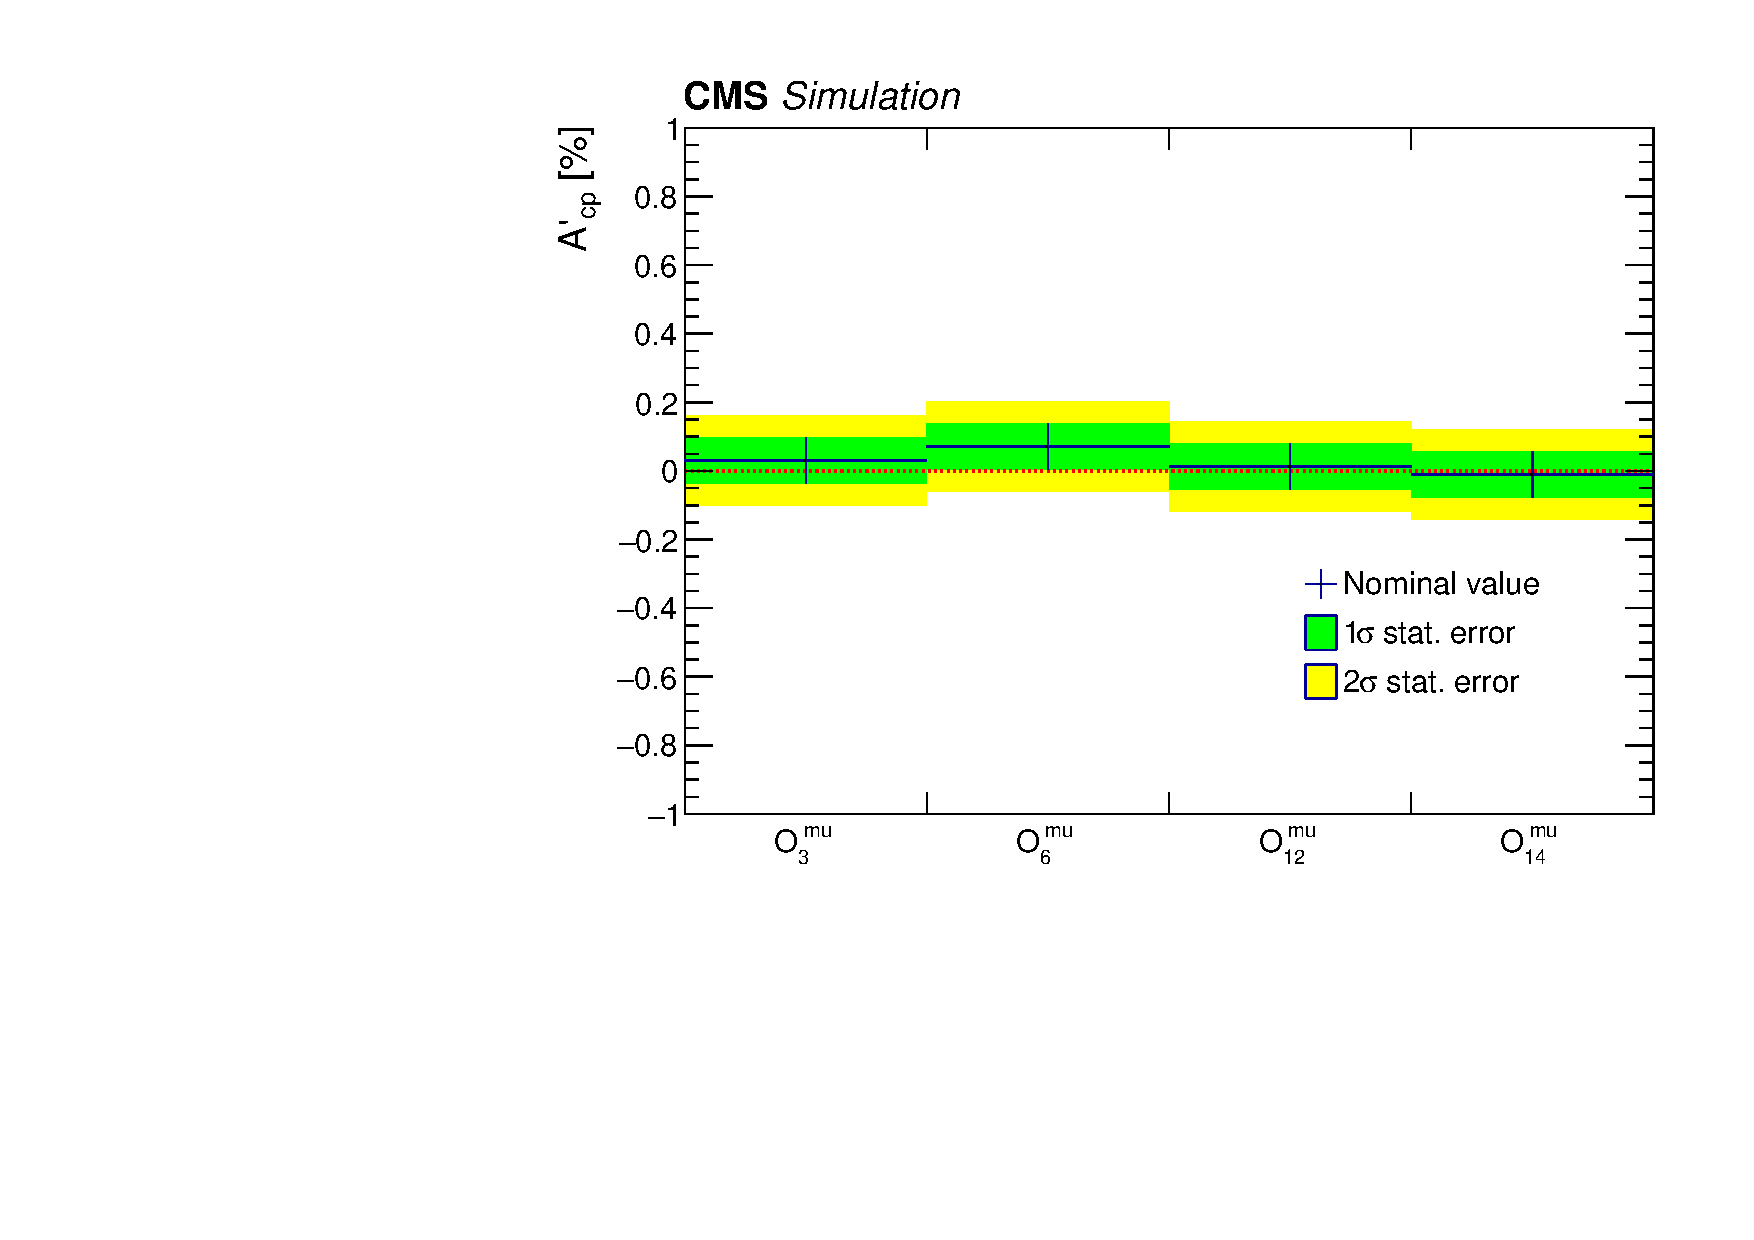
\includegraphics[width=0.45\textwidth]{figure/SimAcp_18_mu_ttbar_chi2_20_opt_150.pdf}
    \caption[The \Acpprime for each observable in SM simulated semileptonic and dileptonic \ttbar events.]
    {
        The \Acpprime for each observable in SM simulated semileptonic and dileptonic \ttbar events for both channels.
        The green(yellow) band is the statistical uncertainty with $1\sigma$($2\sigma$) of the standard deviation(s).
        The electron channel is on the left, and the muon channel is on the right.
        Plots are for 2016, 2017 and 2018 from the top to the bottom separately.
    }
    \label{fig:simulated_signal_acp}
\end{figure}

\begin{figure}
    \centering
    \includegraphics[width=0.45\textwidth]{figure/SimAcp_16_el_background_chi2_20_opt_150.pdf}
    \includegraphics[width=0.45\textwidth]{figure/SimAcp_16_mu_background_chi2_20_opt_150.pdf}
    \includegraphics[width=0.45\textwidth]{figure/SimAcp_17_el_background_chi2_20_opt_150.pdf}
    \includegraphics[width=0.45\textwidth]{figure/SimAcp_17_mu_background_chi2_20_opt_150.pdf}
    \includegraphics[width=0.45\textwidth]{figure/SimAcp_18_el_background_chi2_20_opt_150.pdf}
    \includegraphics[width=0.45\textwidth]{figure/SimAcp_18_mu_background_chi2_20_opt_150.pdf}
    \caption[The \Acpprime for each observable in simulated background events.]
    {
        The \Acpprime for each observable in simulated background events in for both channels.
        The green(yellow) band is the statistical uncertainty with $1\sigma$($2\sigma$) of the standard deviation(s).
        The electron channel is on the left, and the muon channel is on the right.
        Plots are for 2016, 2017 and 2018 from the top to the bottom separately.
    }
    \label{fig:simulated_background_acp}
\end{figure}

\begin{table}
    \caption[The \Acpprime values and their statistical uncertainties in percent for each CP observable.]
    {
        The \Acpprime values and their statistical uncertainties in percent for each CP observable from the electron and muon event-mixing samples and their combination, used to search for detector or reconstruction bias.
    }
    \label{tab:detector_bias}
    \centering\renewcommand\arraystretch{1.2}
    \begin{tabular}{cccc}
        \multicolumn{4}{c}{\Acpprime from event-mixing samples (\%)}\\
        CP observable & \ejets & \mjets & Combined\\
        \hline
        \Othree & $-0.004 \pm 0.004$ & $+0.005 \pm 0.003$ & $+0.003 \pm 0.003$\\
        \Osix & $-0.006 \pm 0.005$ & $+0.003 \pm 0.003$ & $+0.003 \pm 0.003$\\
        \Otwelve & $+0.005 \pm 0.005$ & $-0.001 \pm 0.003$ & $+0.001 \pm 0.002$\\
        \Ofourteen & $-0.008 \pm 0.004$ & $-0.001 \pm 0.003$ & $-0.005 \pm 0.002$\\
    \end{tabular}
\end{table}

\begin{figure}
    \centering
    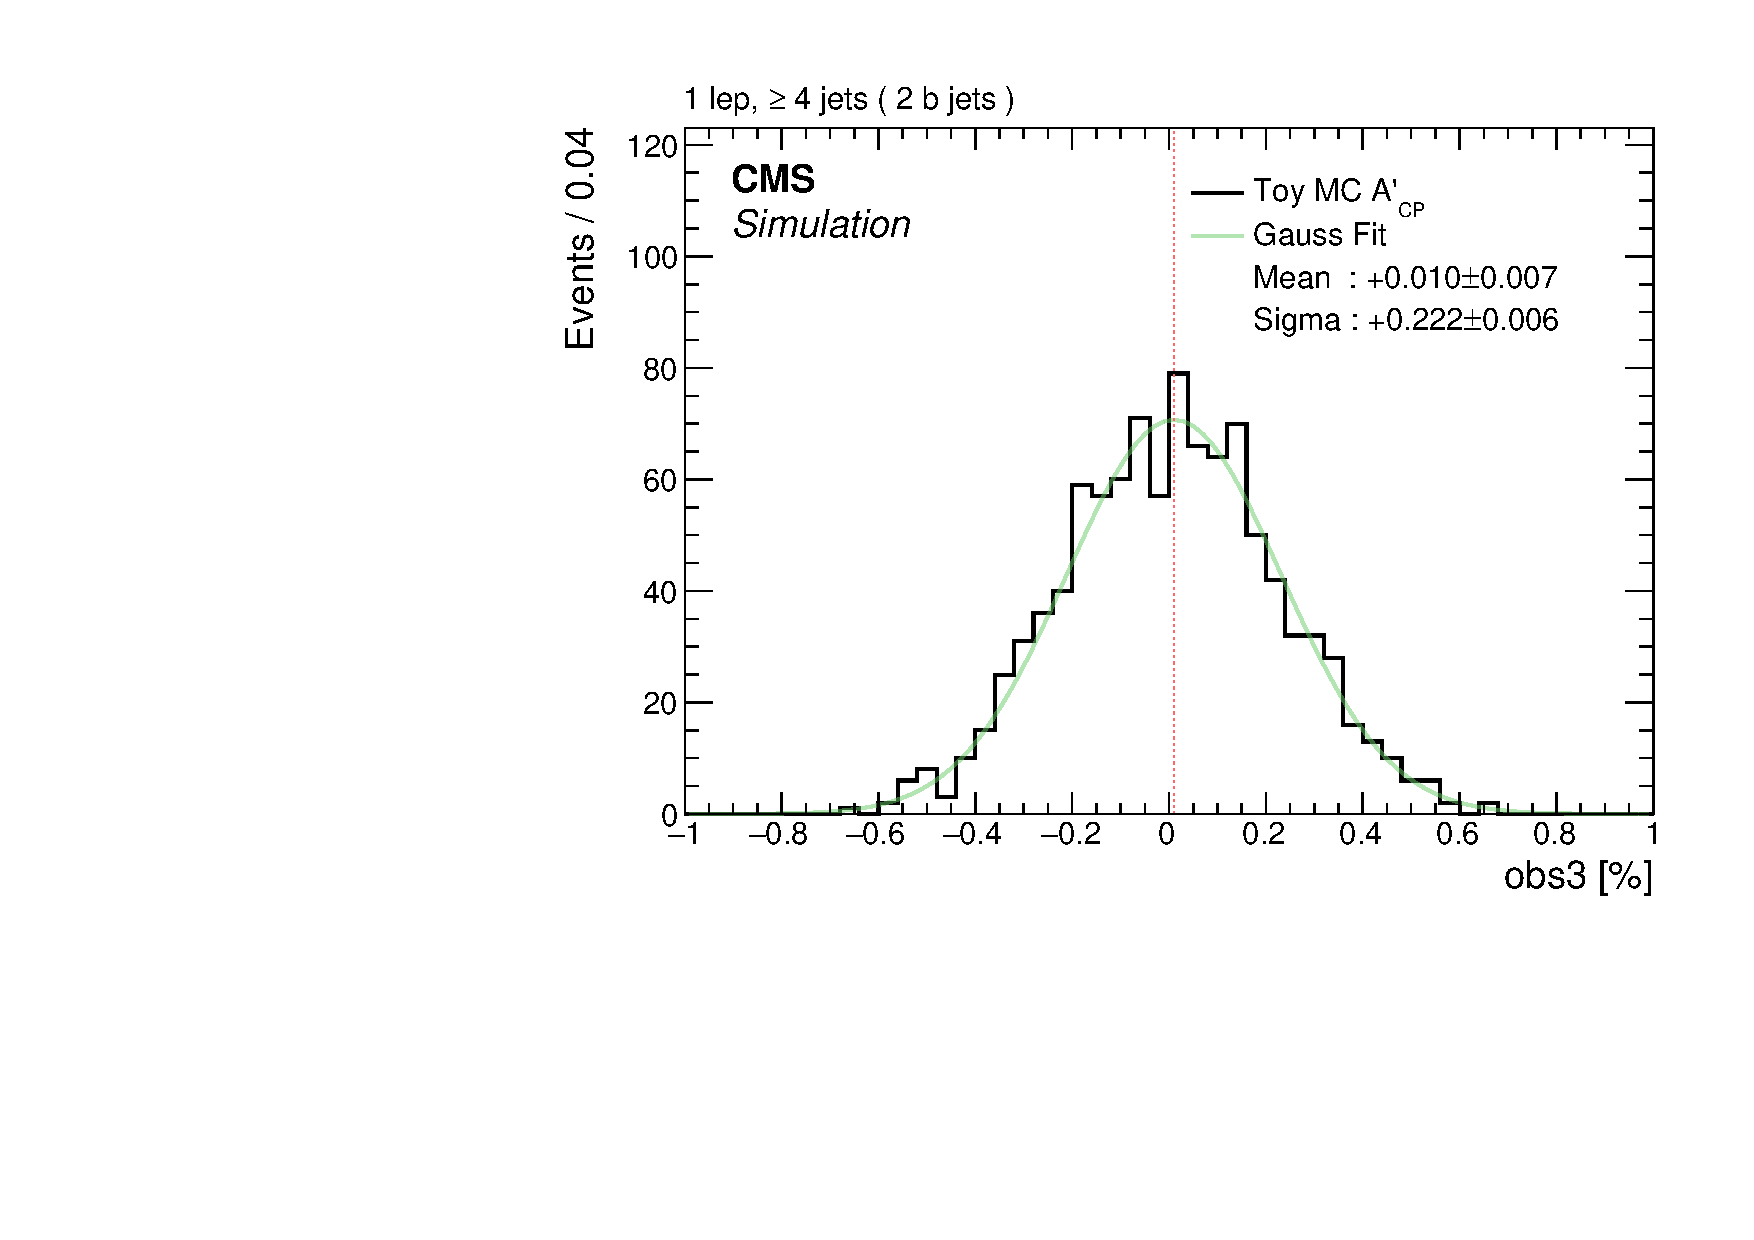
\includegraphics[width=0.45\textwidth]{figure/SimAcp_RunII_co_obs3.pdf}
    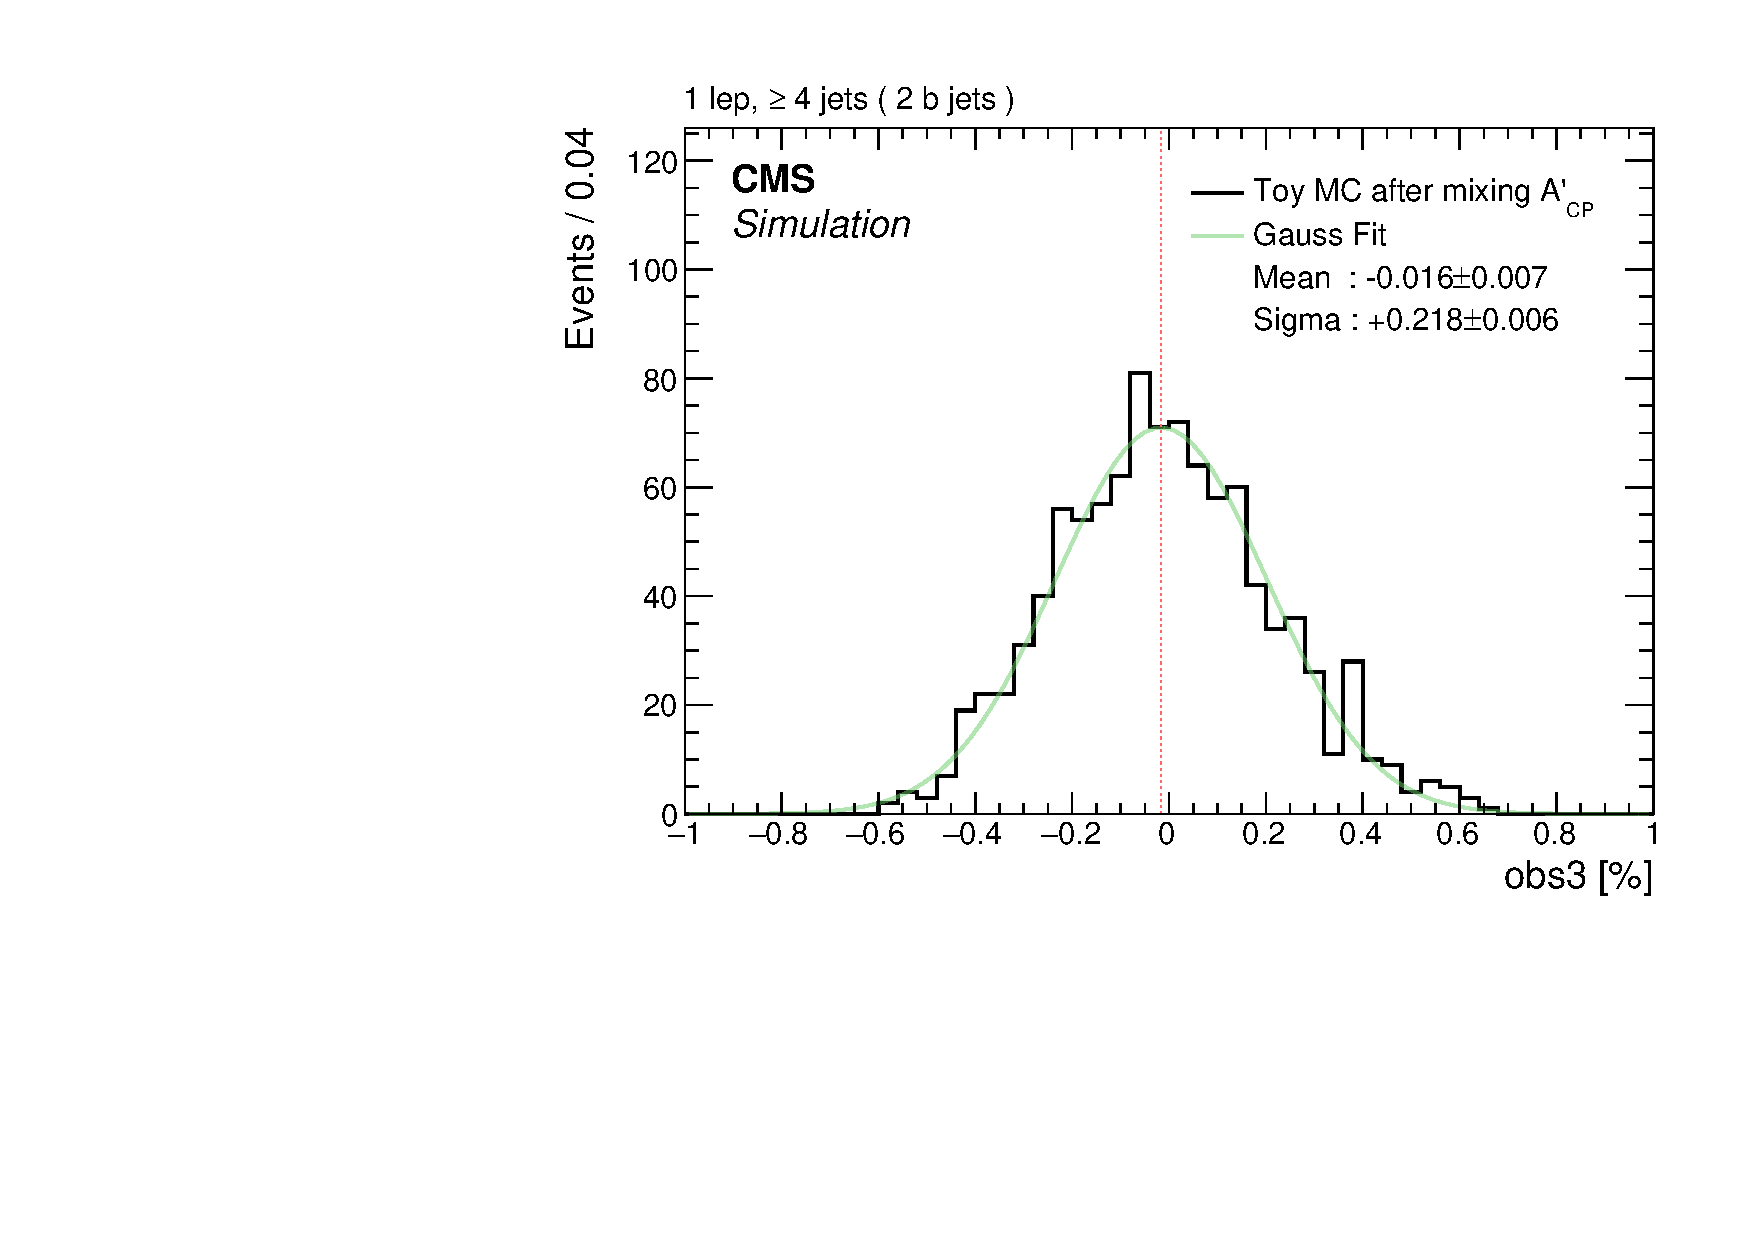
\includegraphics[width=0.45\textwidth]{figure/SimAcp_RunII_co_obs3_mixed.pdf}
    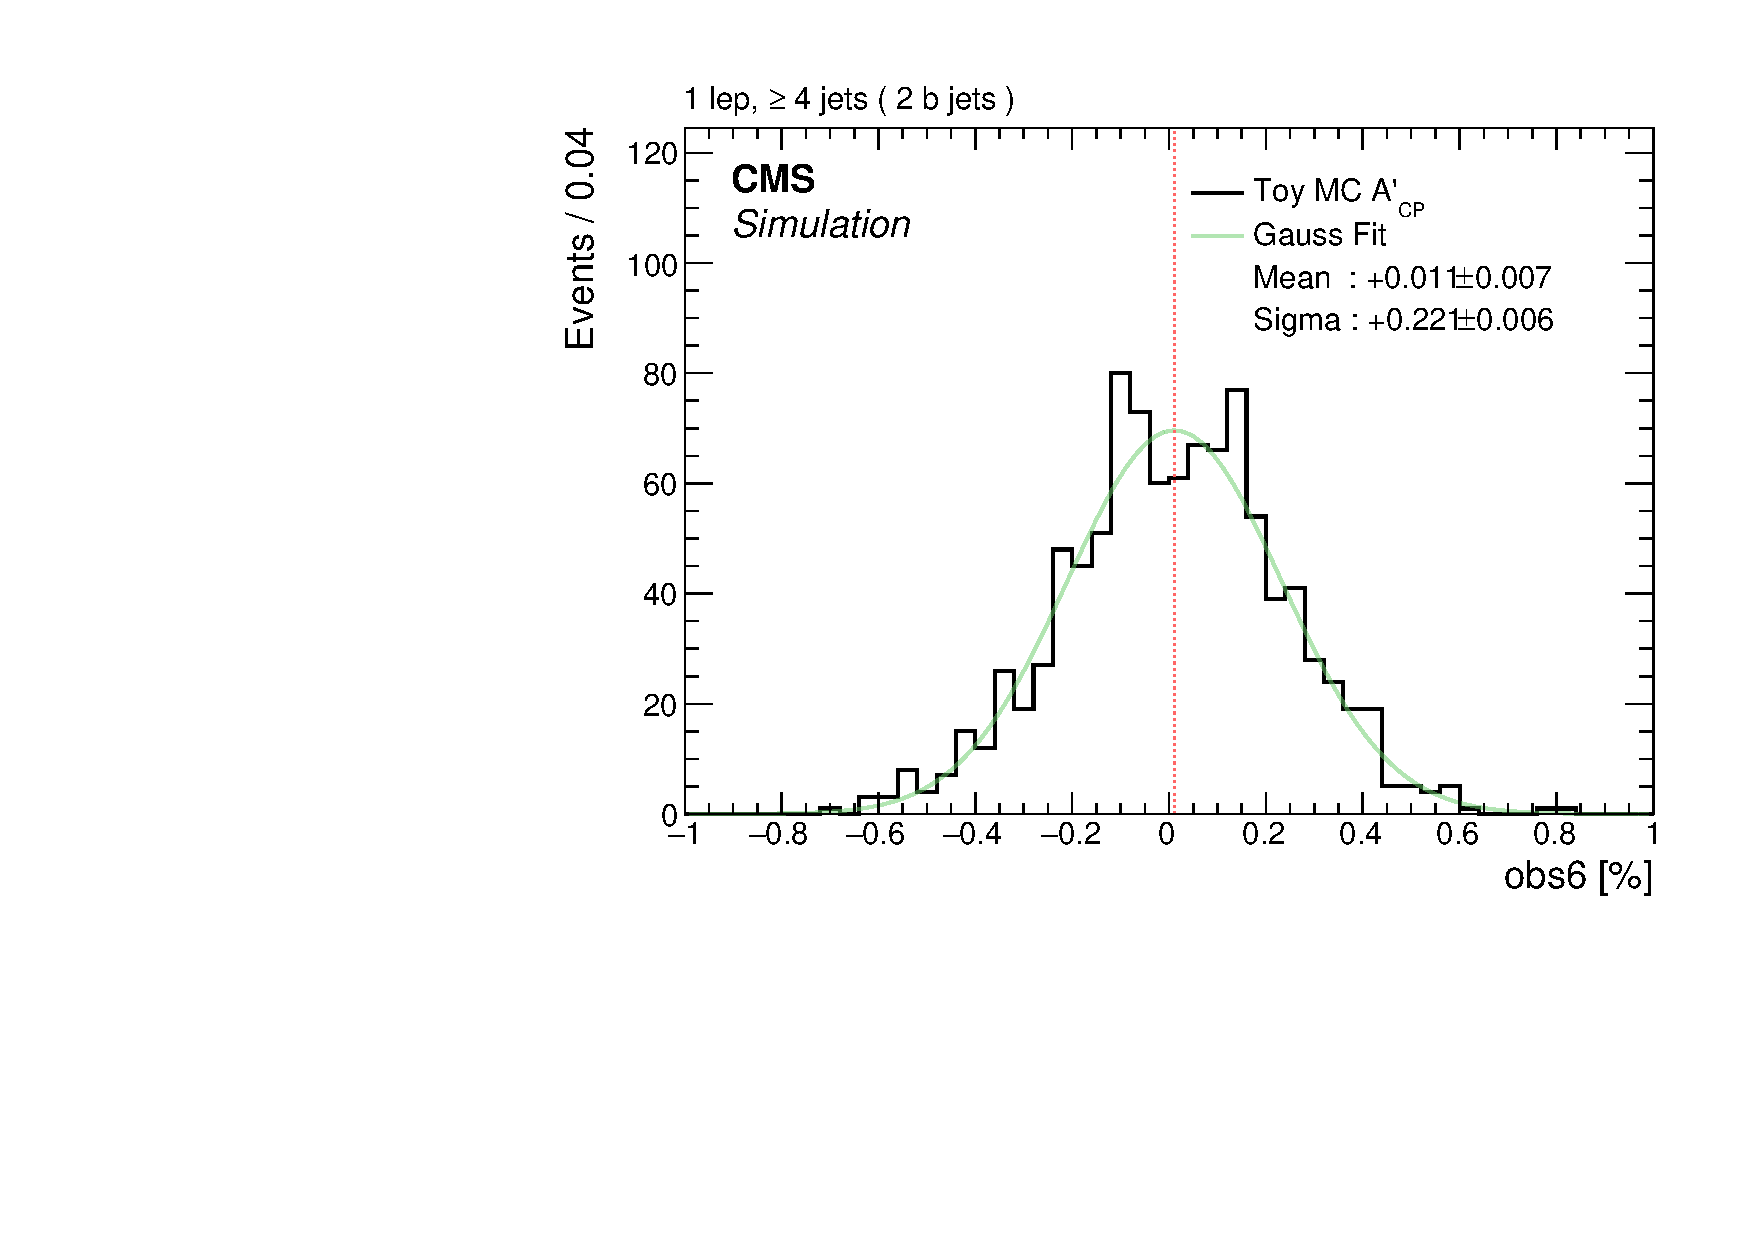
\includegraphics[width=0.45\textwidth]{figure/SimAcp_RunII_co_obs6.pdf}
    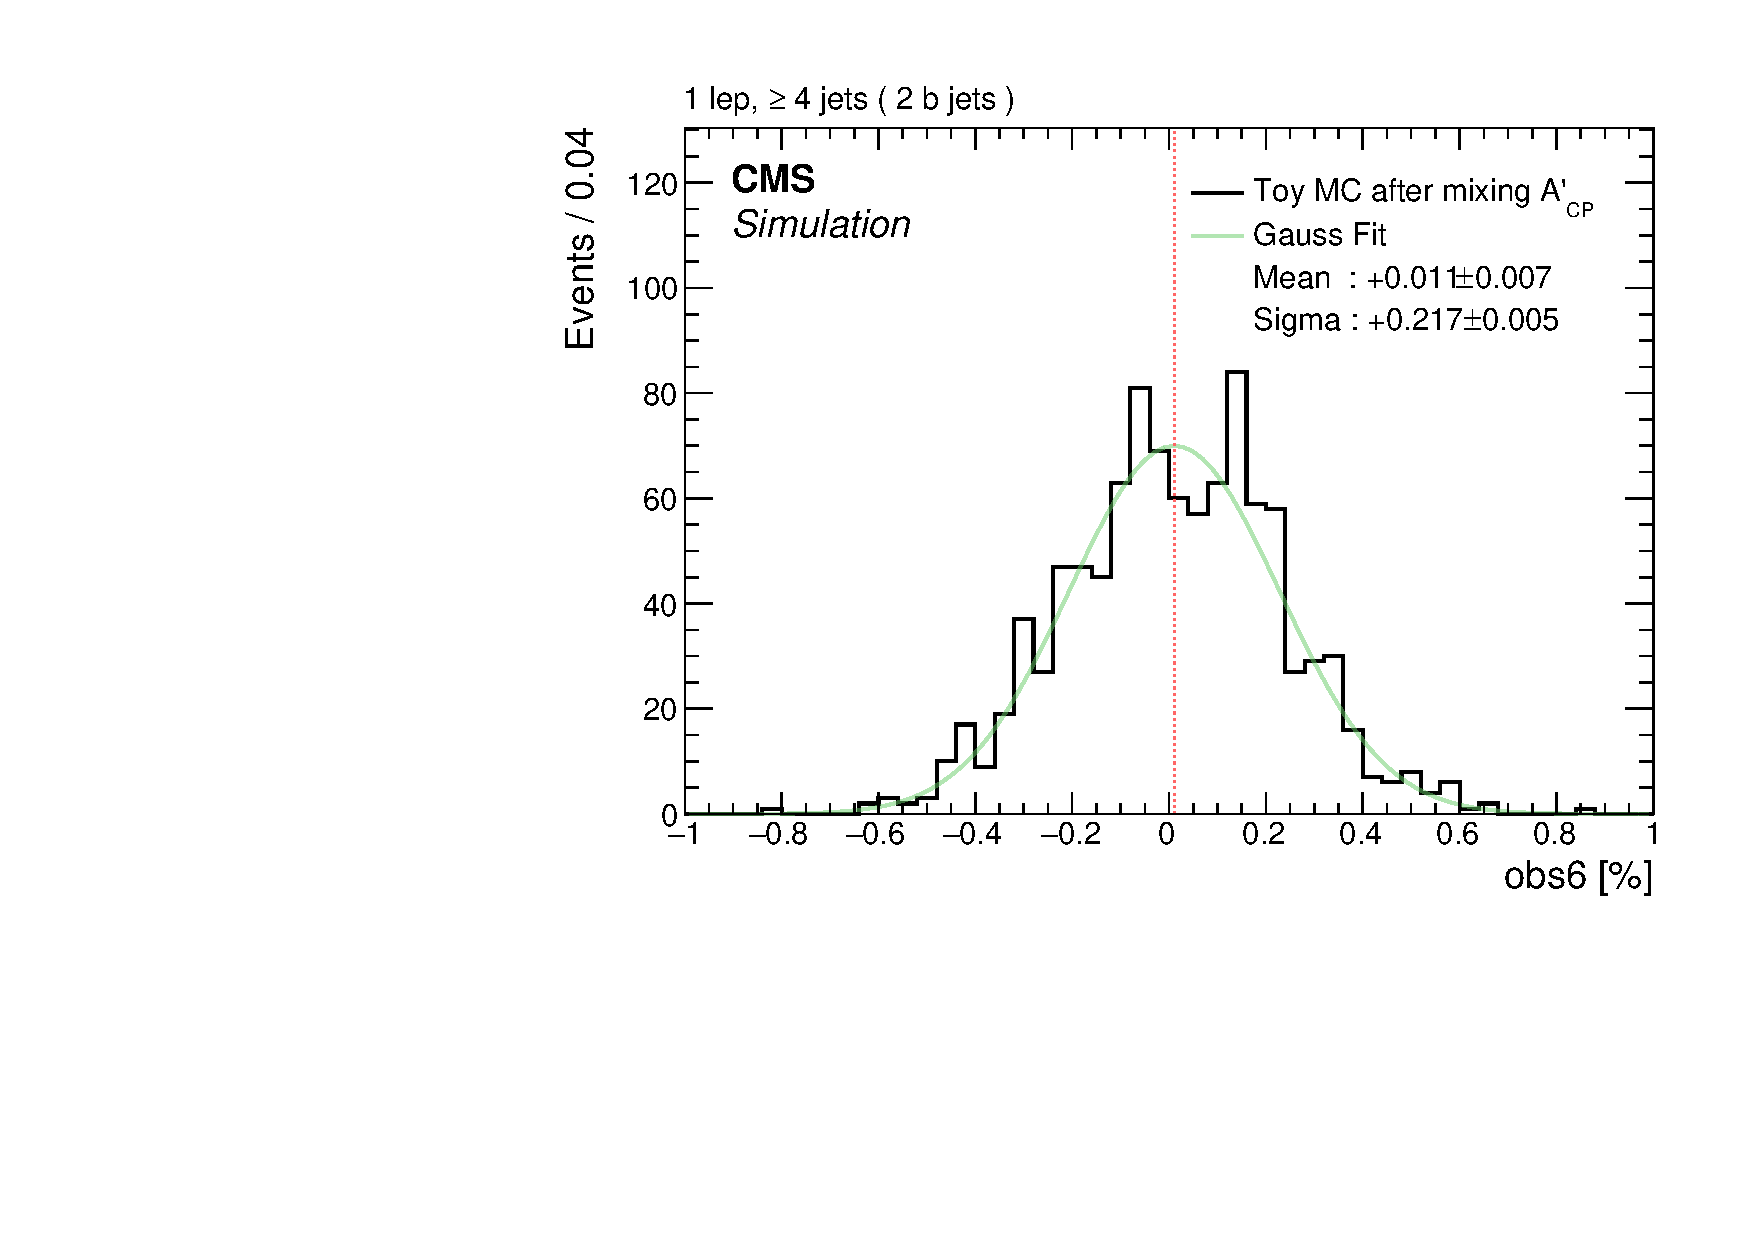
\includegraphics[width=0.45\textwidth]{figure/SimAcp_RunII_co_obs6_mixed.pdf}
    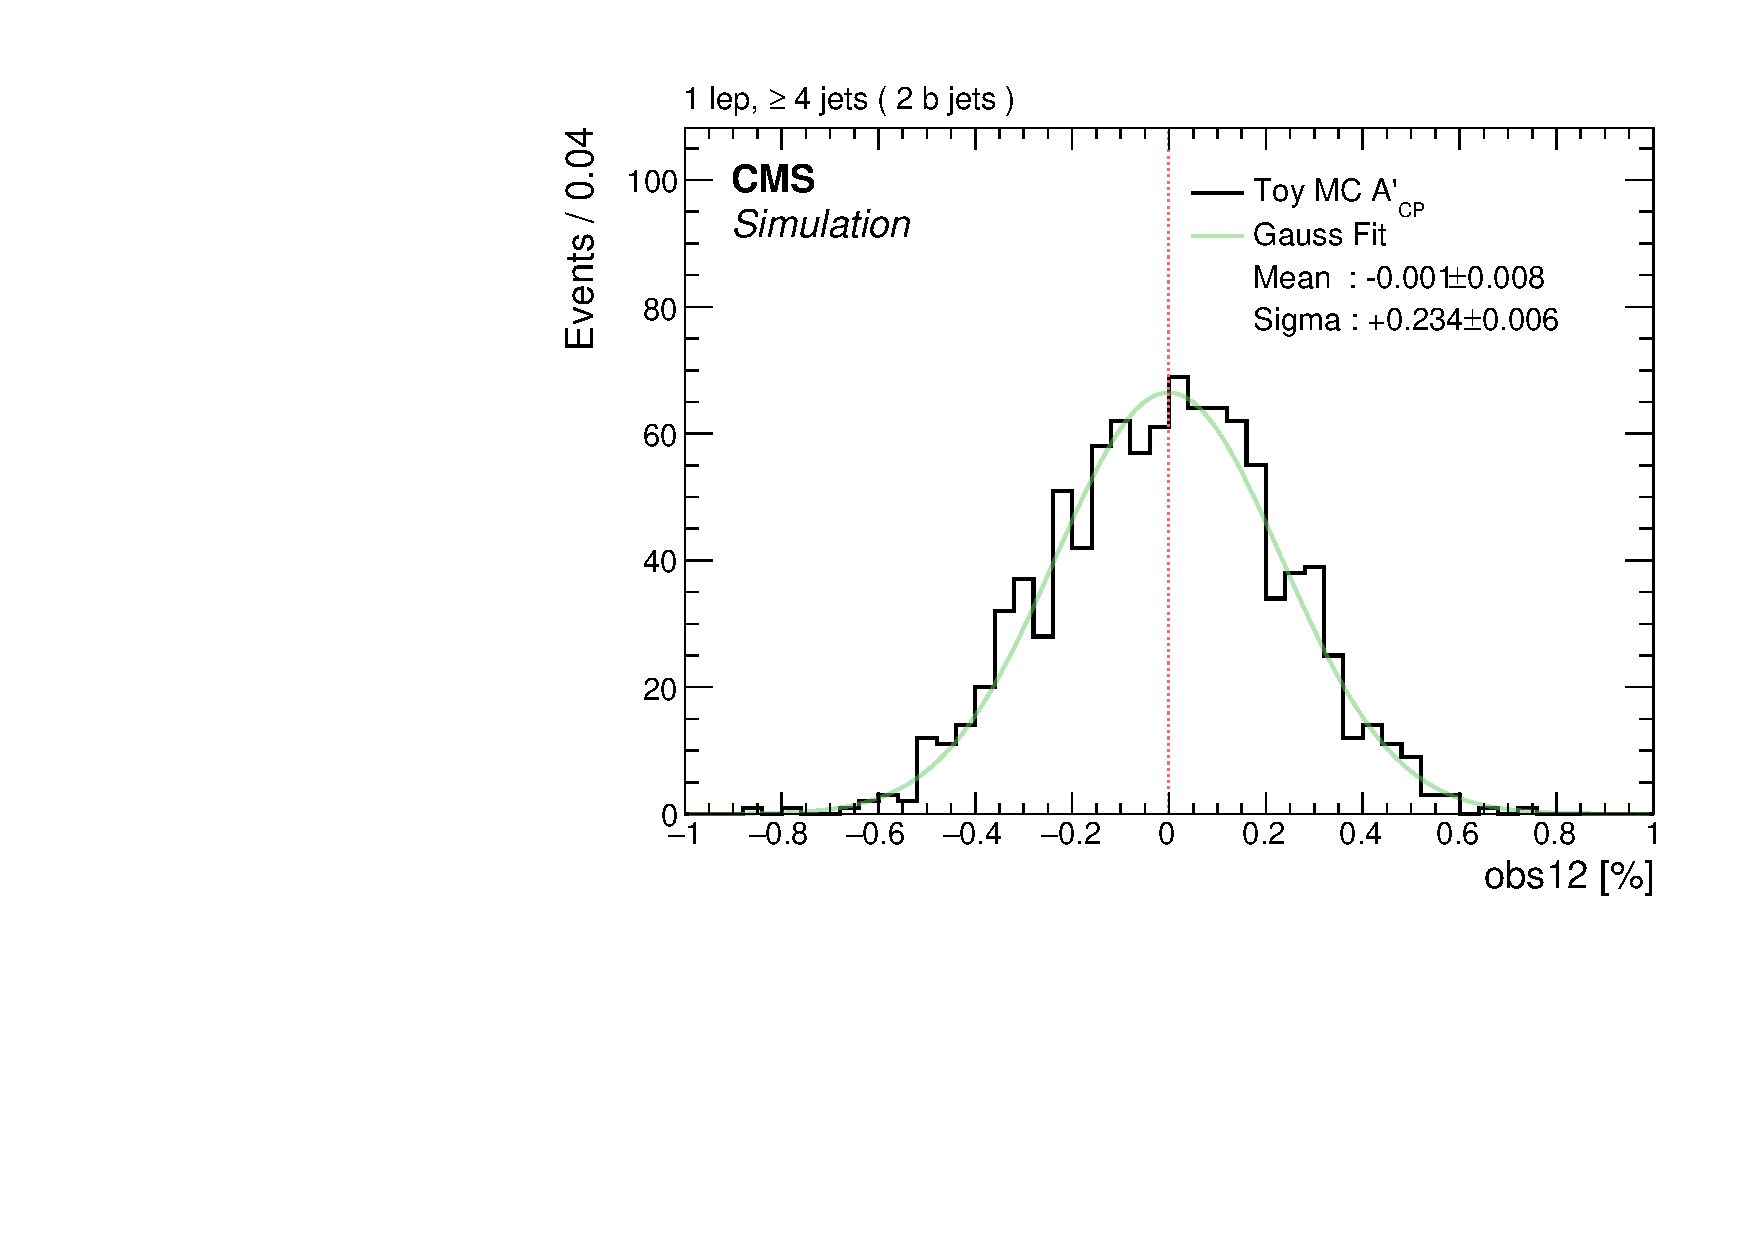
\includegraphics[width=0.45\textwidth]{figure/SimAcp_RunII_co_obs12.pdf}
    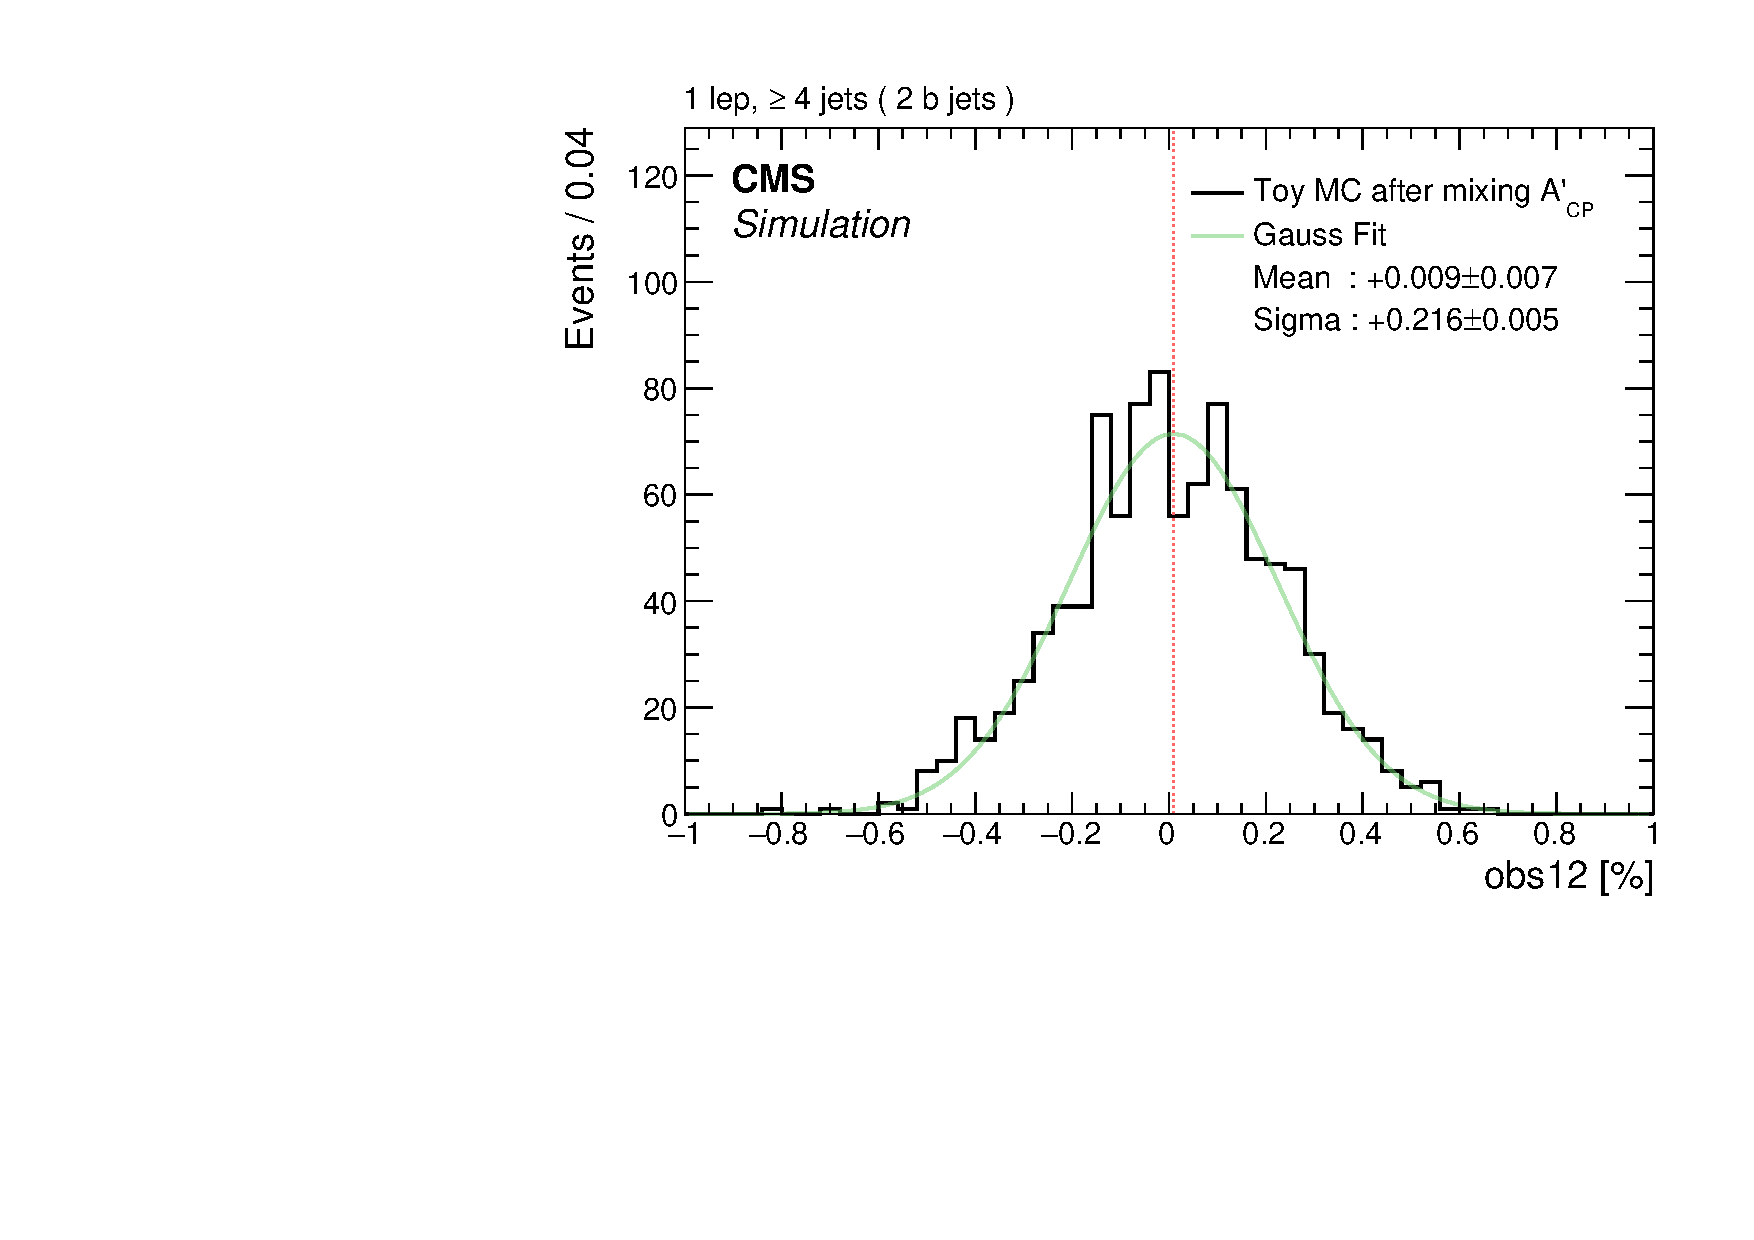
\includegraphics[width=0.45\textwidth]{figure/SimAcp_RunII_co_obs12_mixed.pdf}
    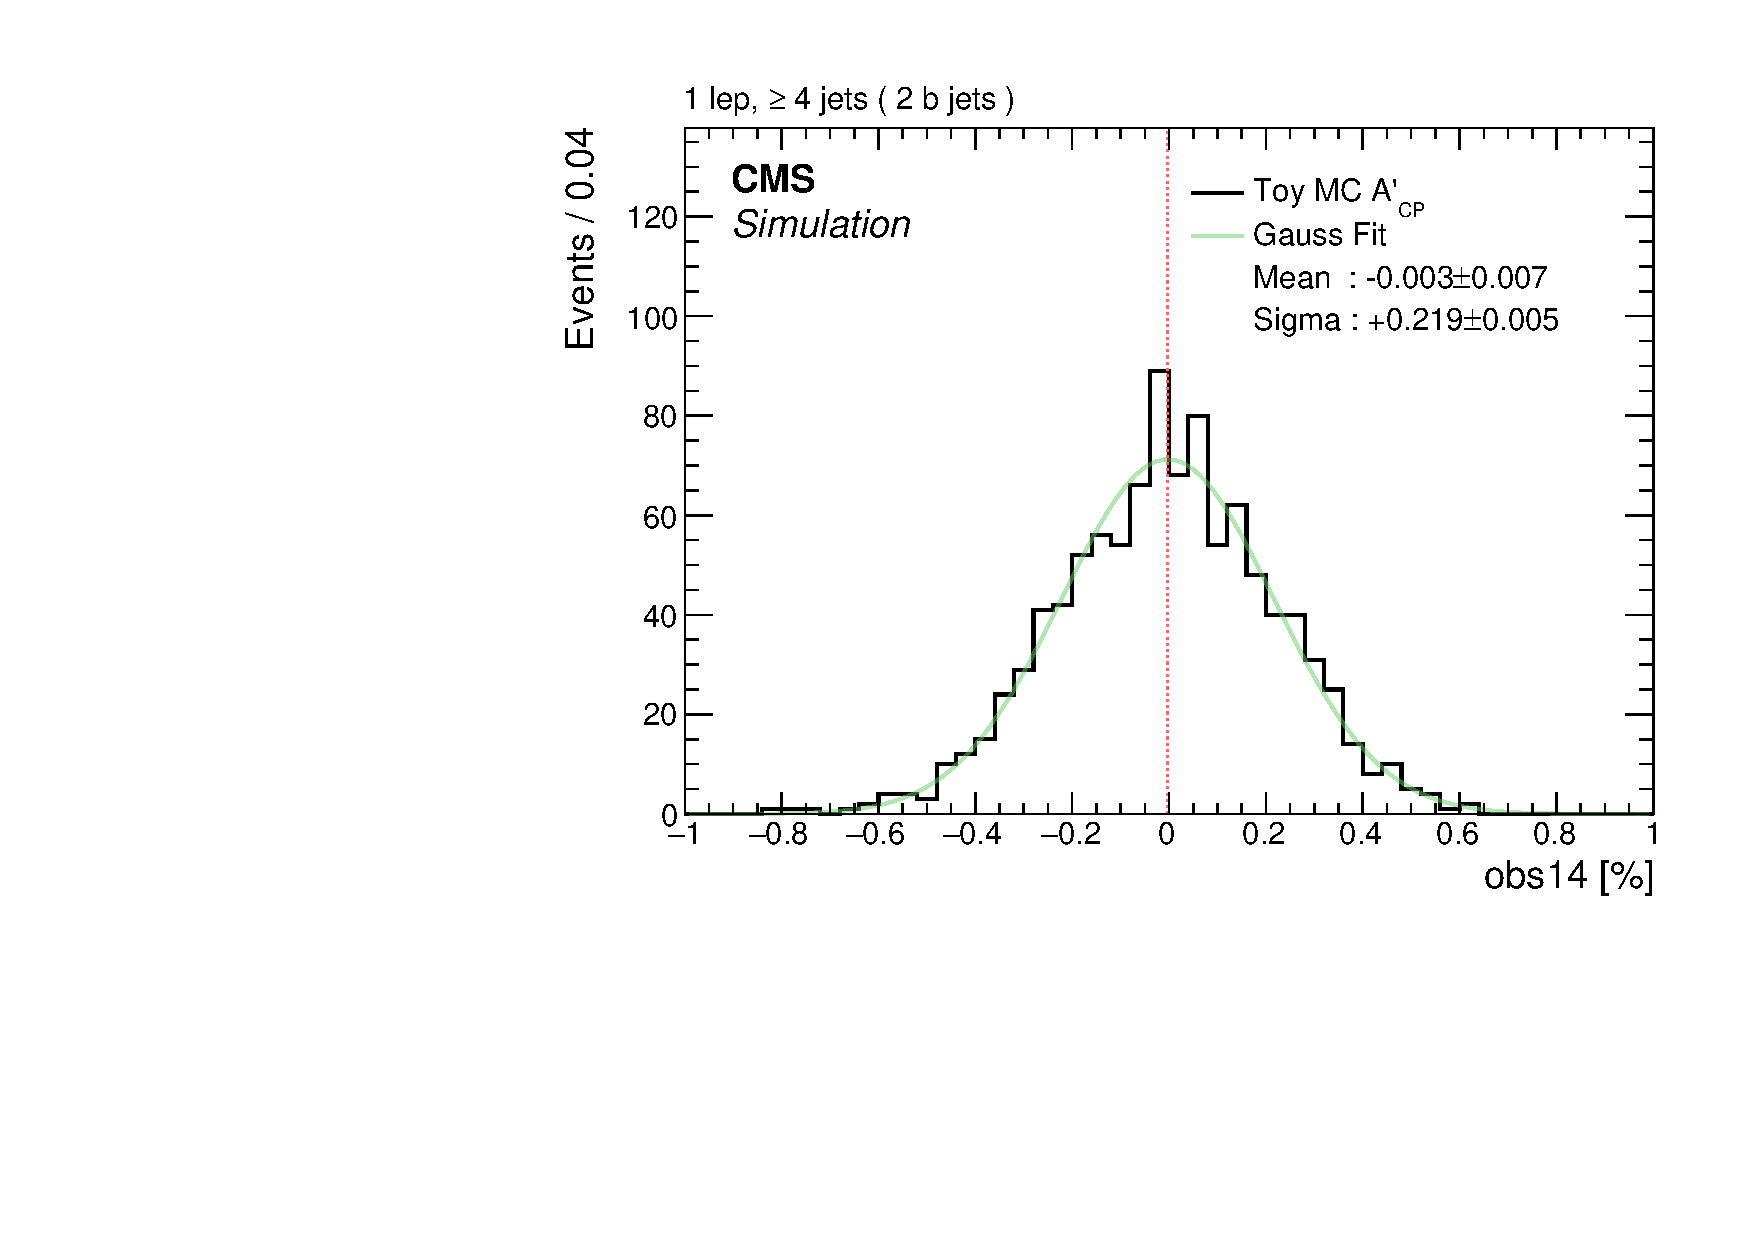
\includegraphics[width=0.45\textwidth]{figure/SimAcp_RunII_co_obs14.pdf}
    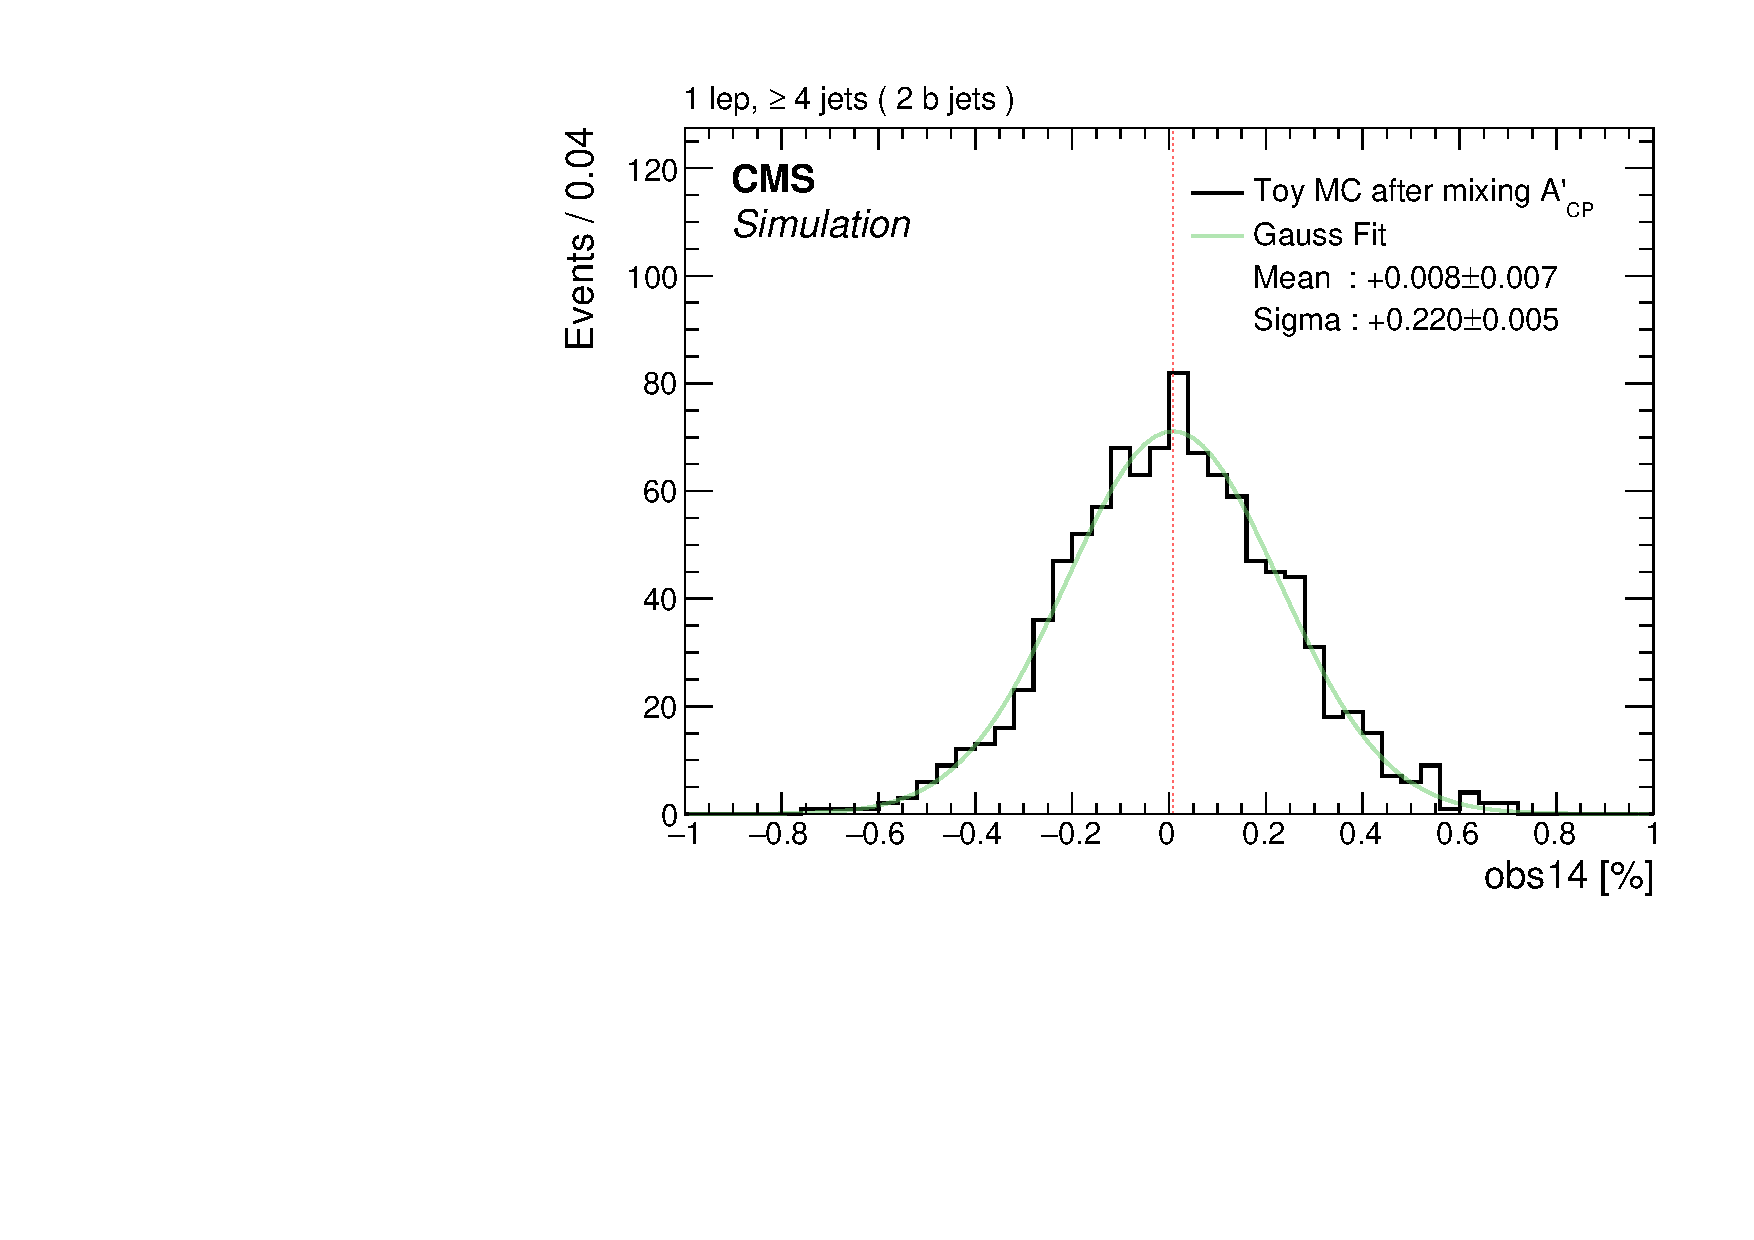
\includegraphics[width=0.45\textwidth]{figure/SimAcp_RunII_co_obs14_mixed.pdf}
    \caption[The \Acpprime for each observable in SM simulated \ttbar samples and mixed samples.]
    {
        The \Acpprime for each observable in SM simulated \ttbar samples (left) and mixed samples (right).
        The green line is the fitted gaussian and the red dotted line presents the mean value of the gaussian.
    }
    \label{fig:correlation_study}
\end{figure}

\begin{figure}
    \centering
    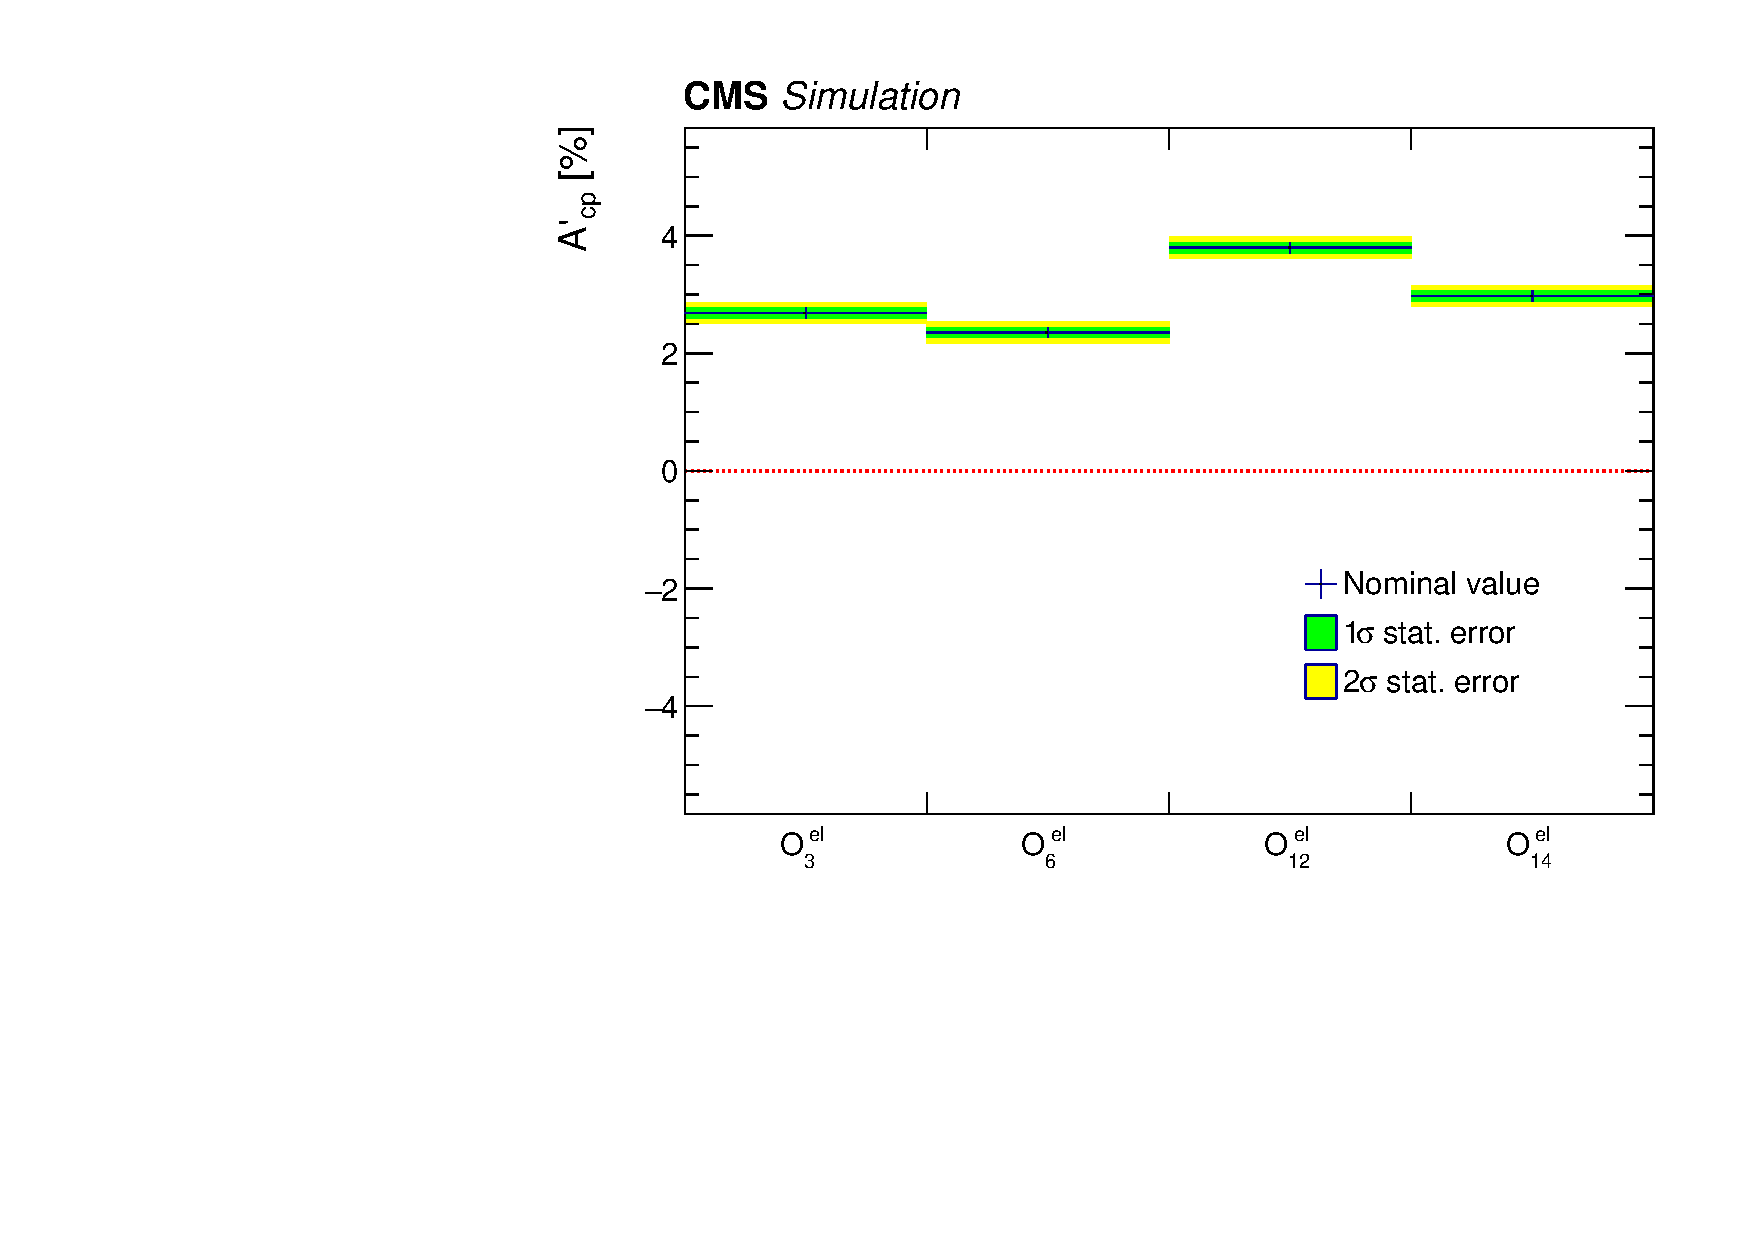
\includegraphics[width=0.45\textwidth]{figure/SimAcp_16_el_ttbar_Acp_10.pdf}
    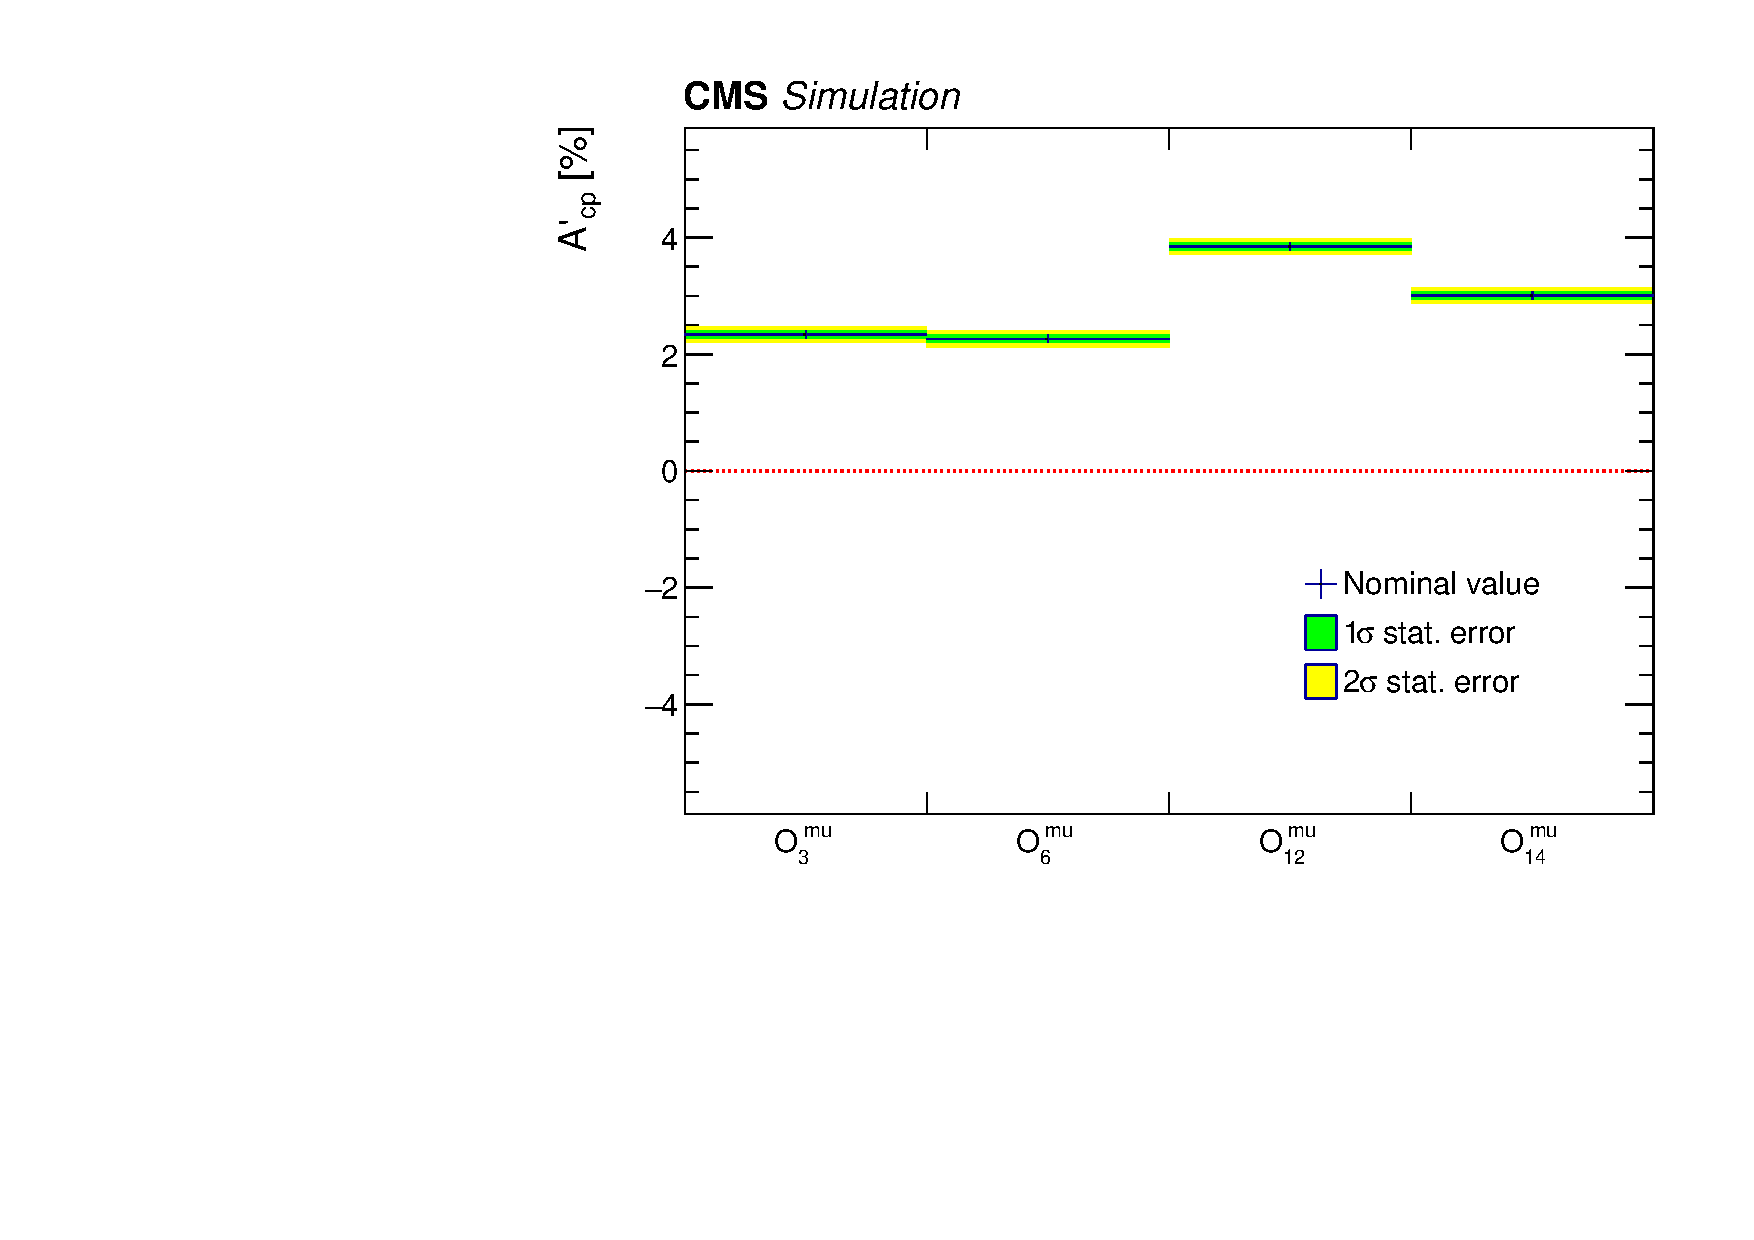
\includegraphics[width=0.45\textwidth]{figure/SimAcp_16_mu_ttbar_Acp_10.pdf}
    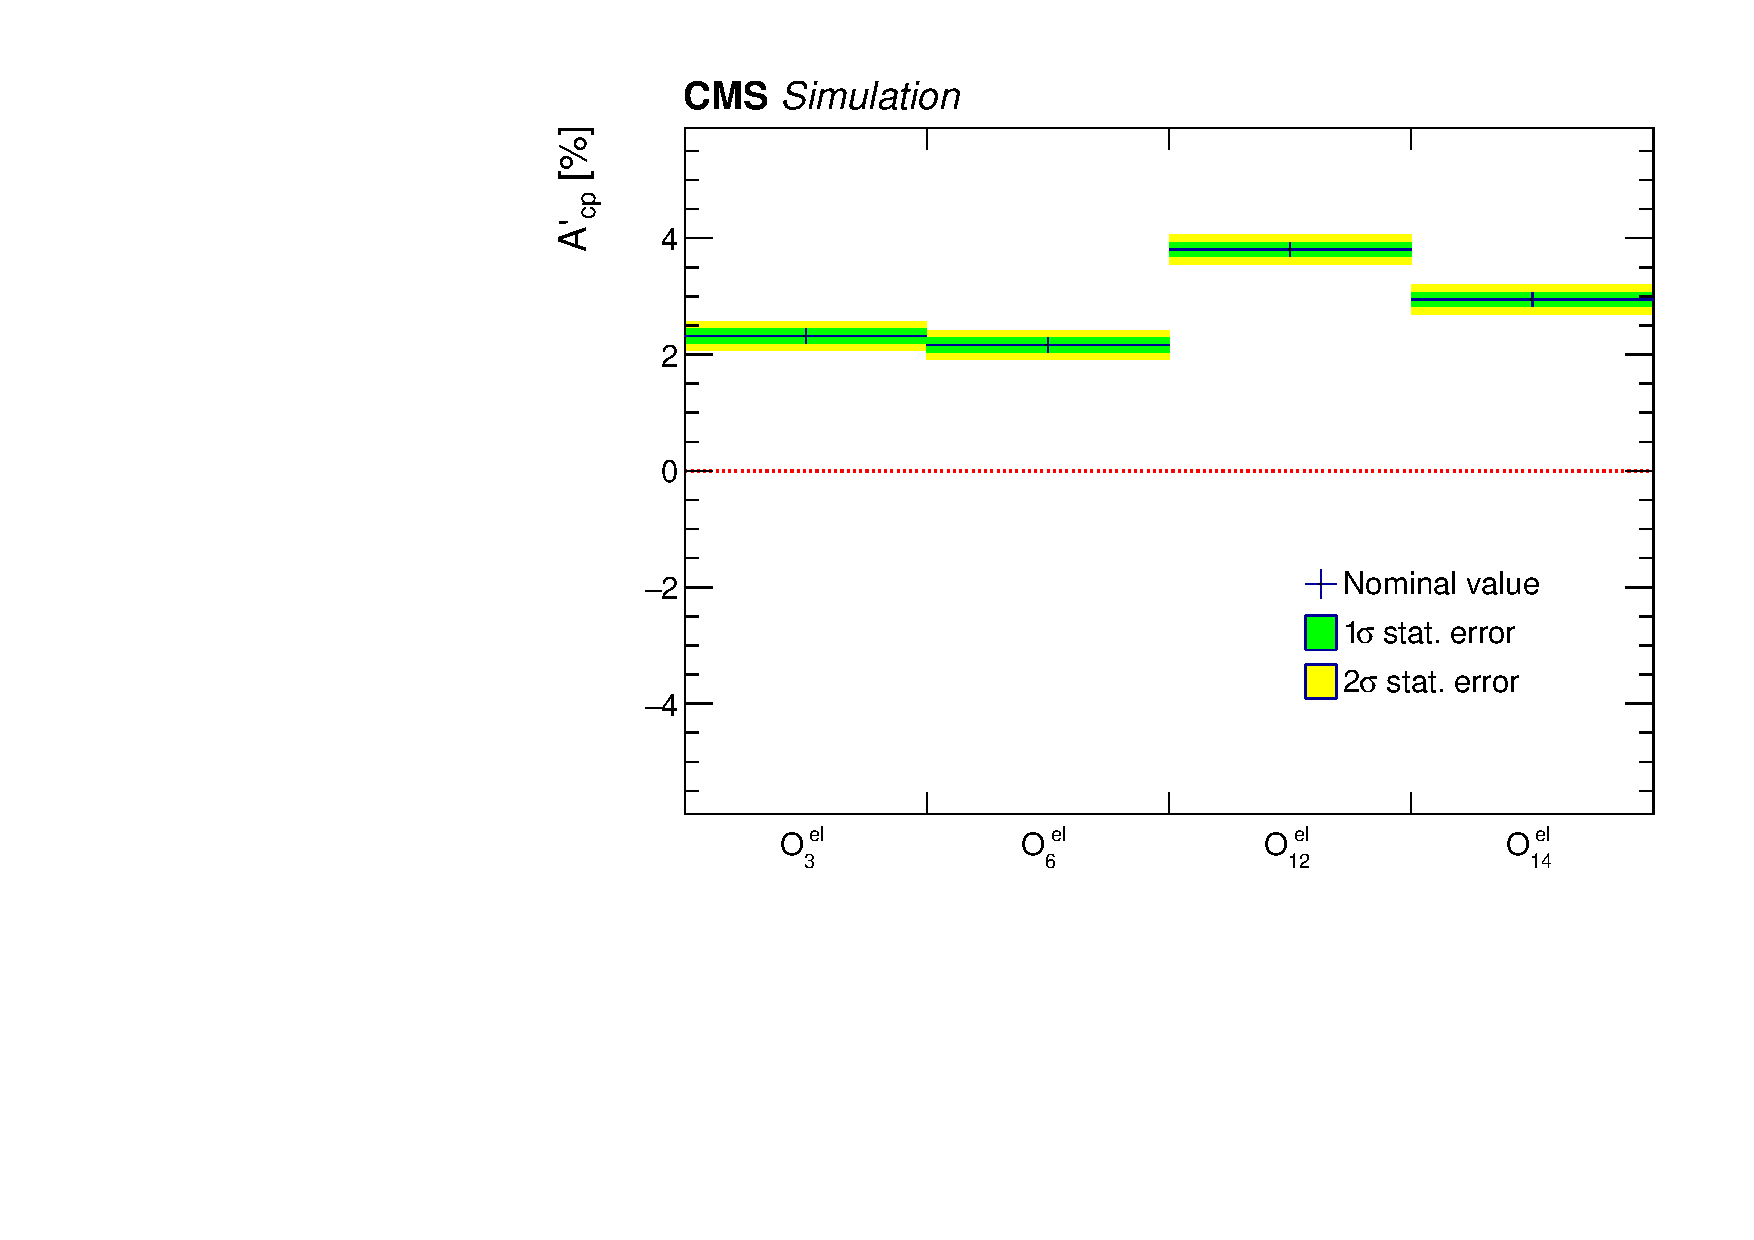
\includegraphics[width=0.45\textwidth]{figure/SimAcp_17_el_ttbar_Acp_10.pdf}
    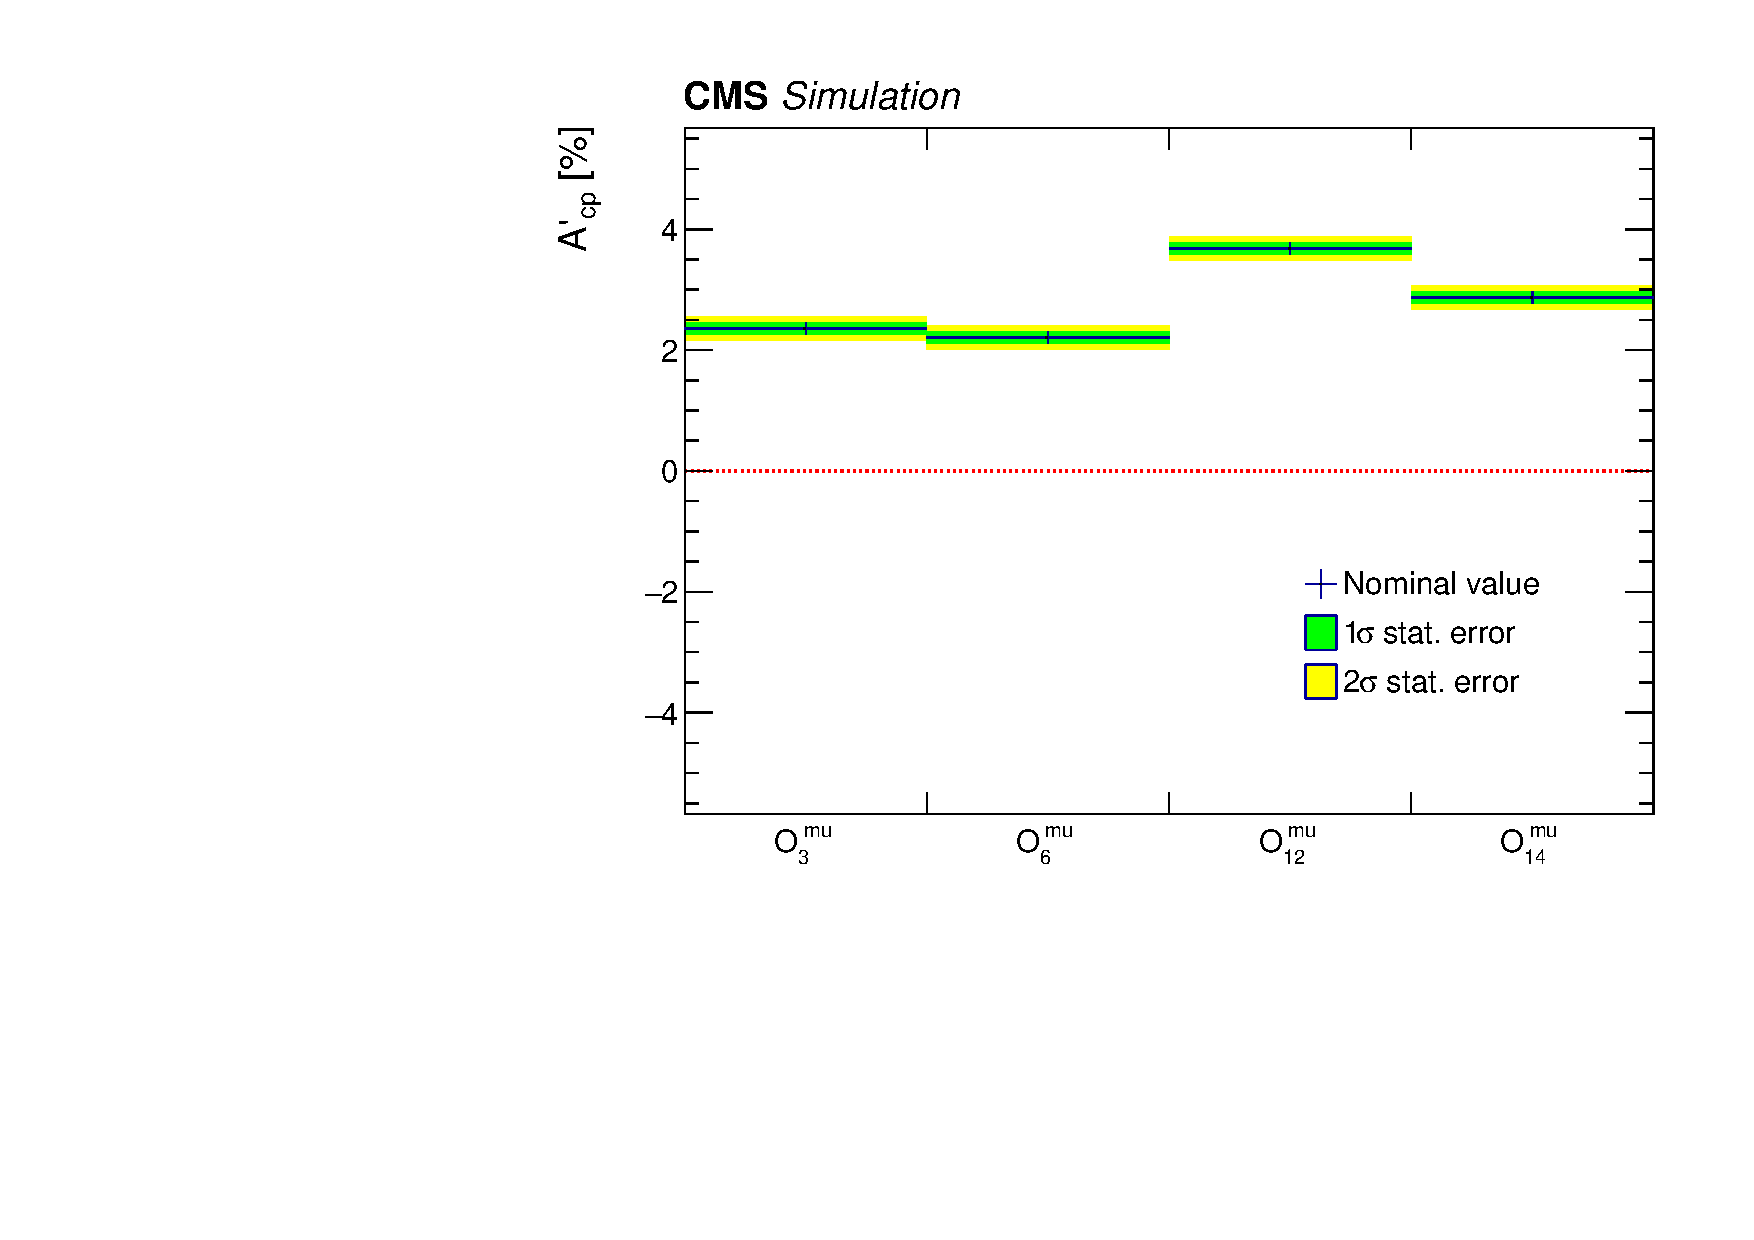
\includegraphics[width=0.45\textwidth]{figure/SimAcp_17_mu_ttbar_Acp_10.pdf}
    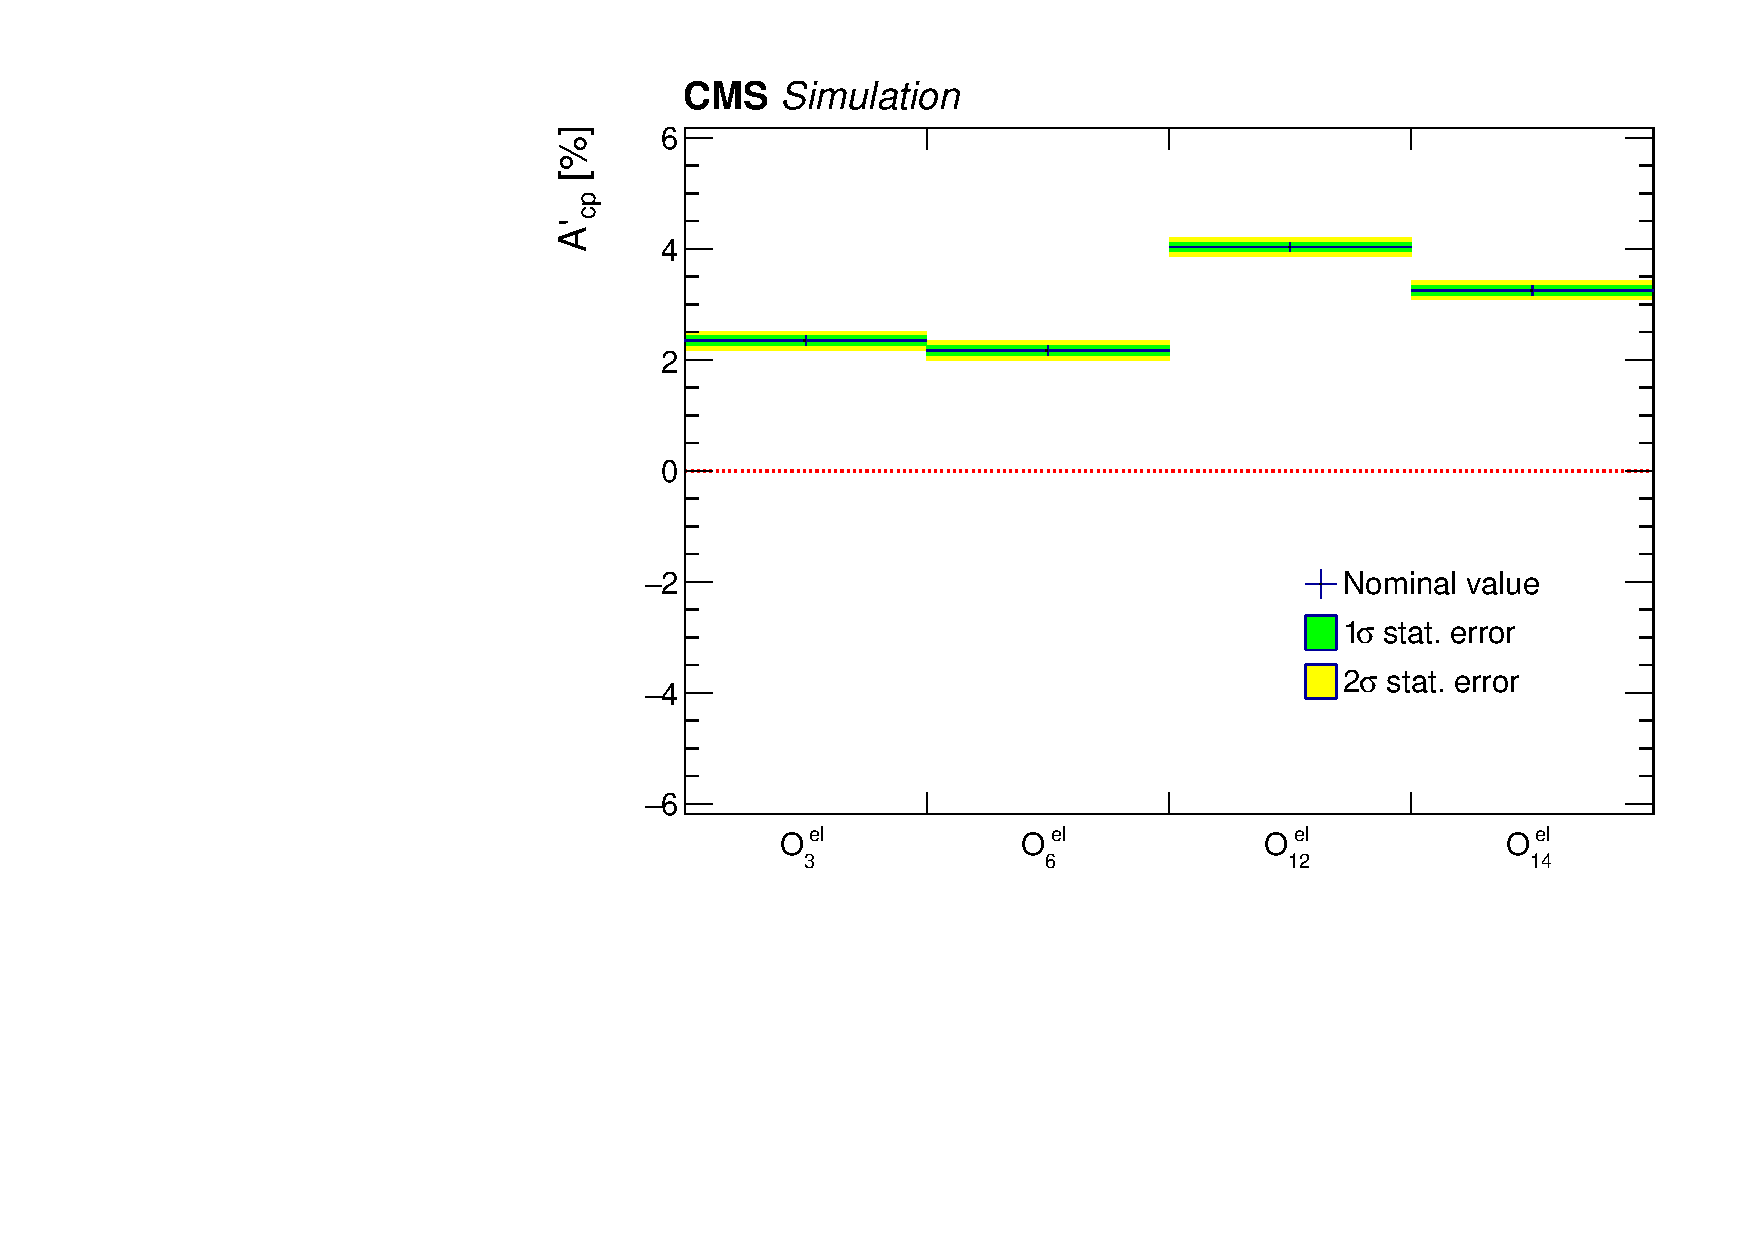
\includegraphics[width=0.45\textwidth]{figure/SimAcp_18_el_ttbar_Acp_10.pdf}
    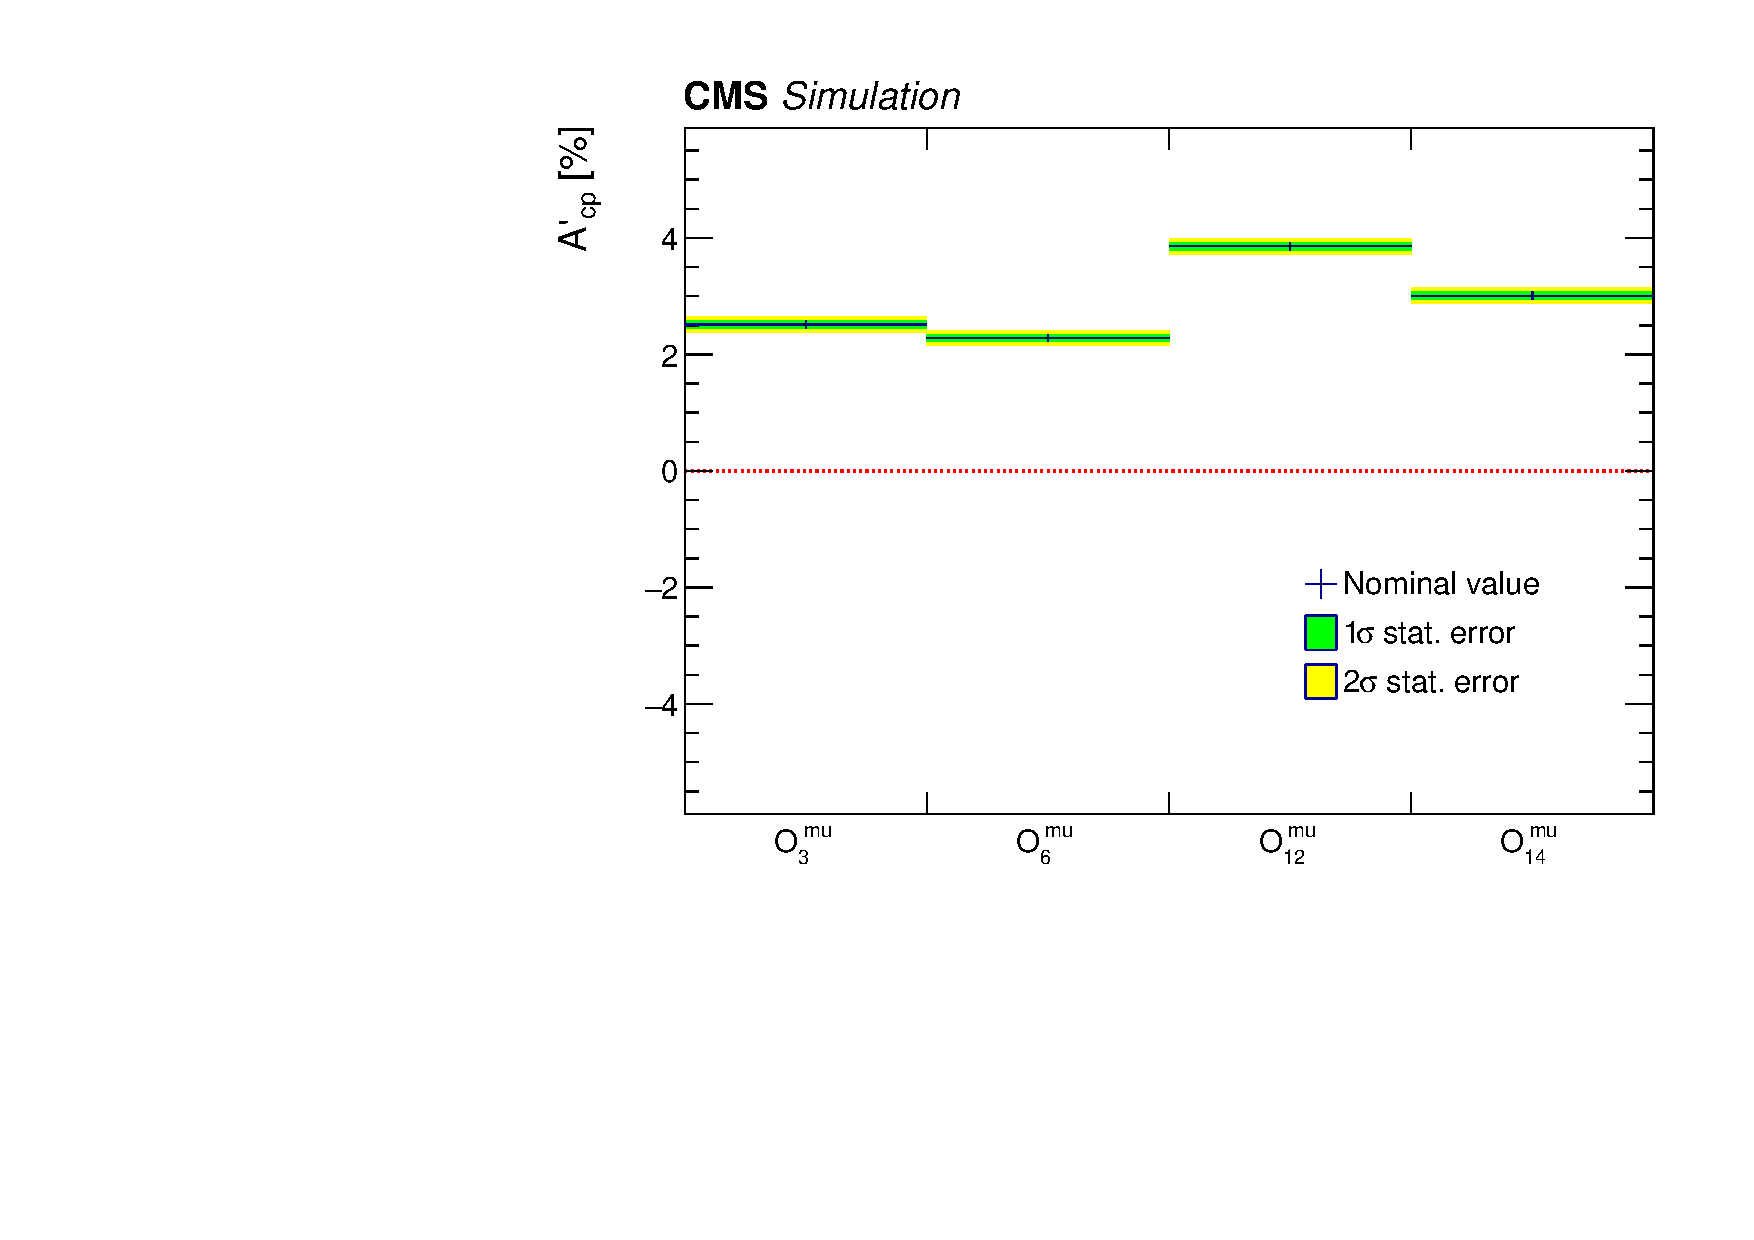
\includegraphics[width=0.45\textwidth]{figure/SimAcp_18_mu_ttbar_Acp_10.pdf}
    \caption[The \Acpprime for each observable in SM simulated semileptonic \ttbar events.]
    {
        The \Acpprime for each observable in SM simulated semileptonic \ttbar events in signal region after adding artificial \Acp for both channels.
        The green(yellow) band is the statistical uncertainty with $1\sigma$($2\sigma$) of the standard deviation(s).
        The electron channel is on the left, and the muon channel is on the right.
        Plots are for 2016, 2017 and 2018 from the top to the bottom separately.
    }
    \label{fig:artificial_acp}
\end{figure}

\begin{figure}
    \centering
    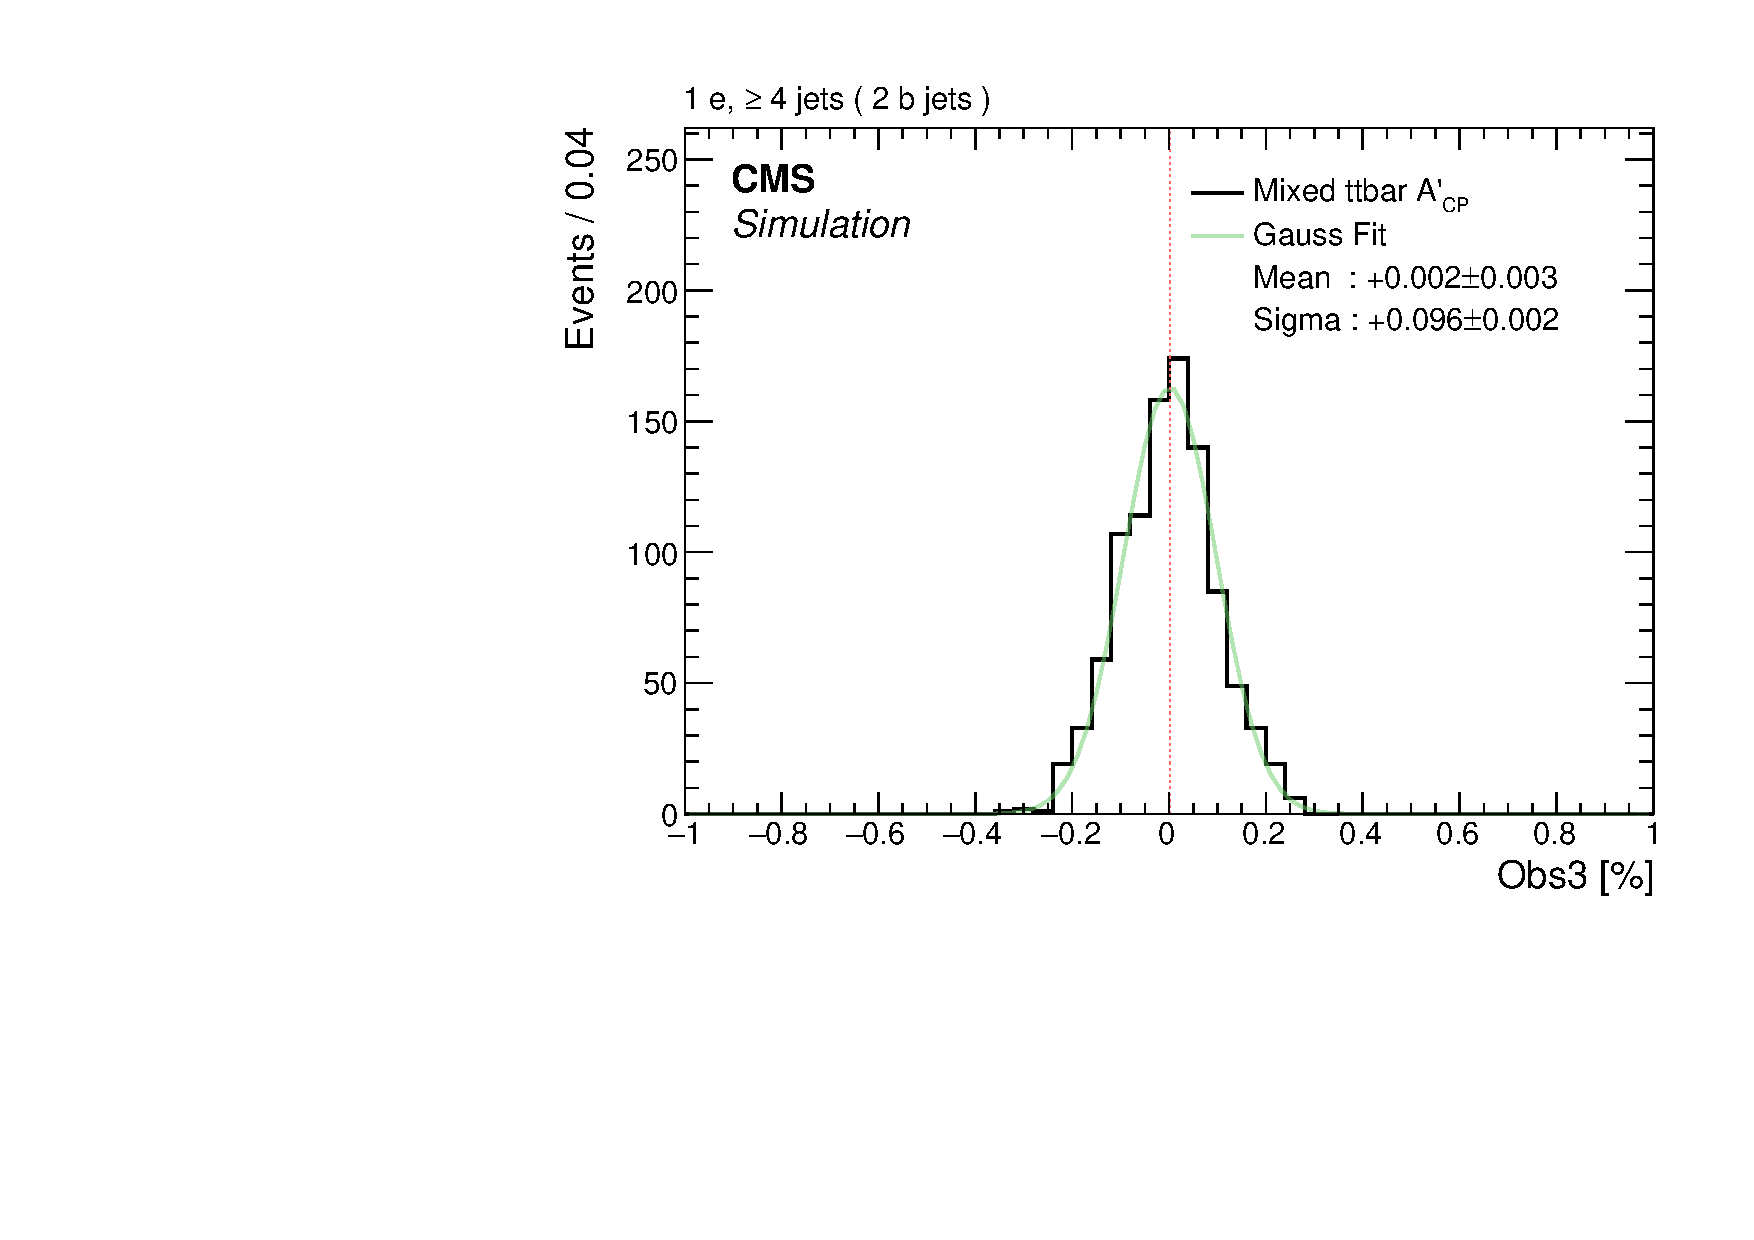
\includegraphics[width=0.45\textwidth]{figure/SimAcp_16_el_Obs3_Acp_10_mixed.pdf}
    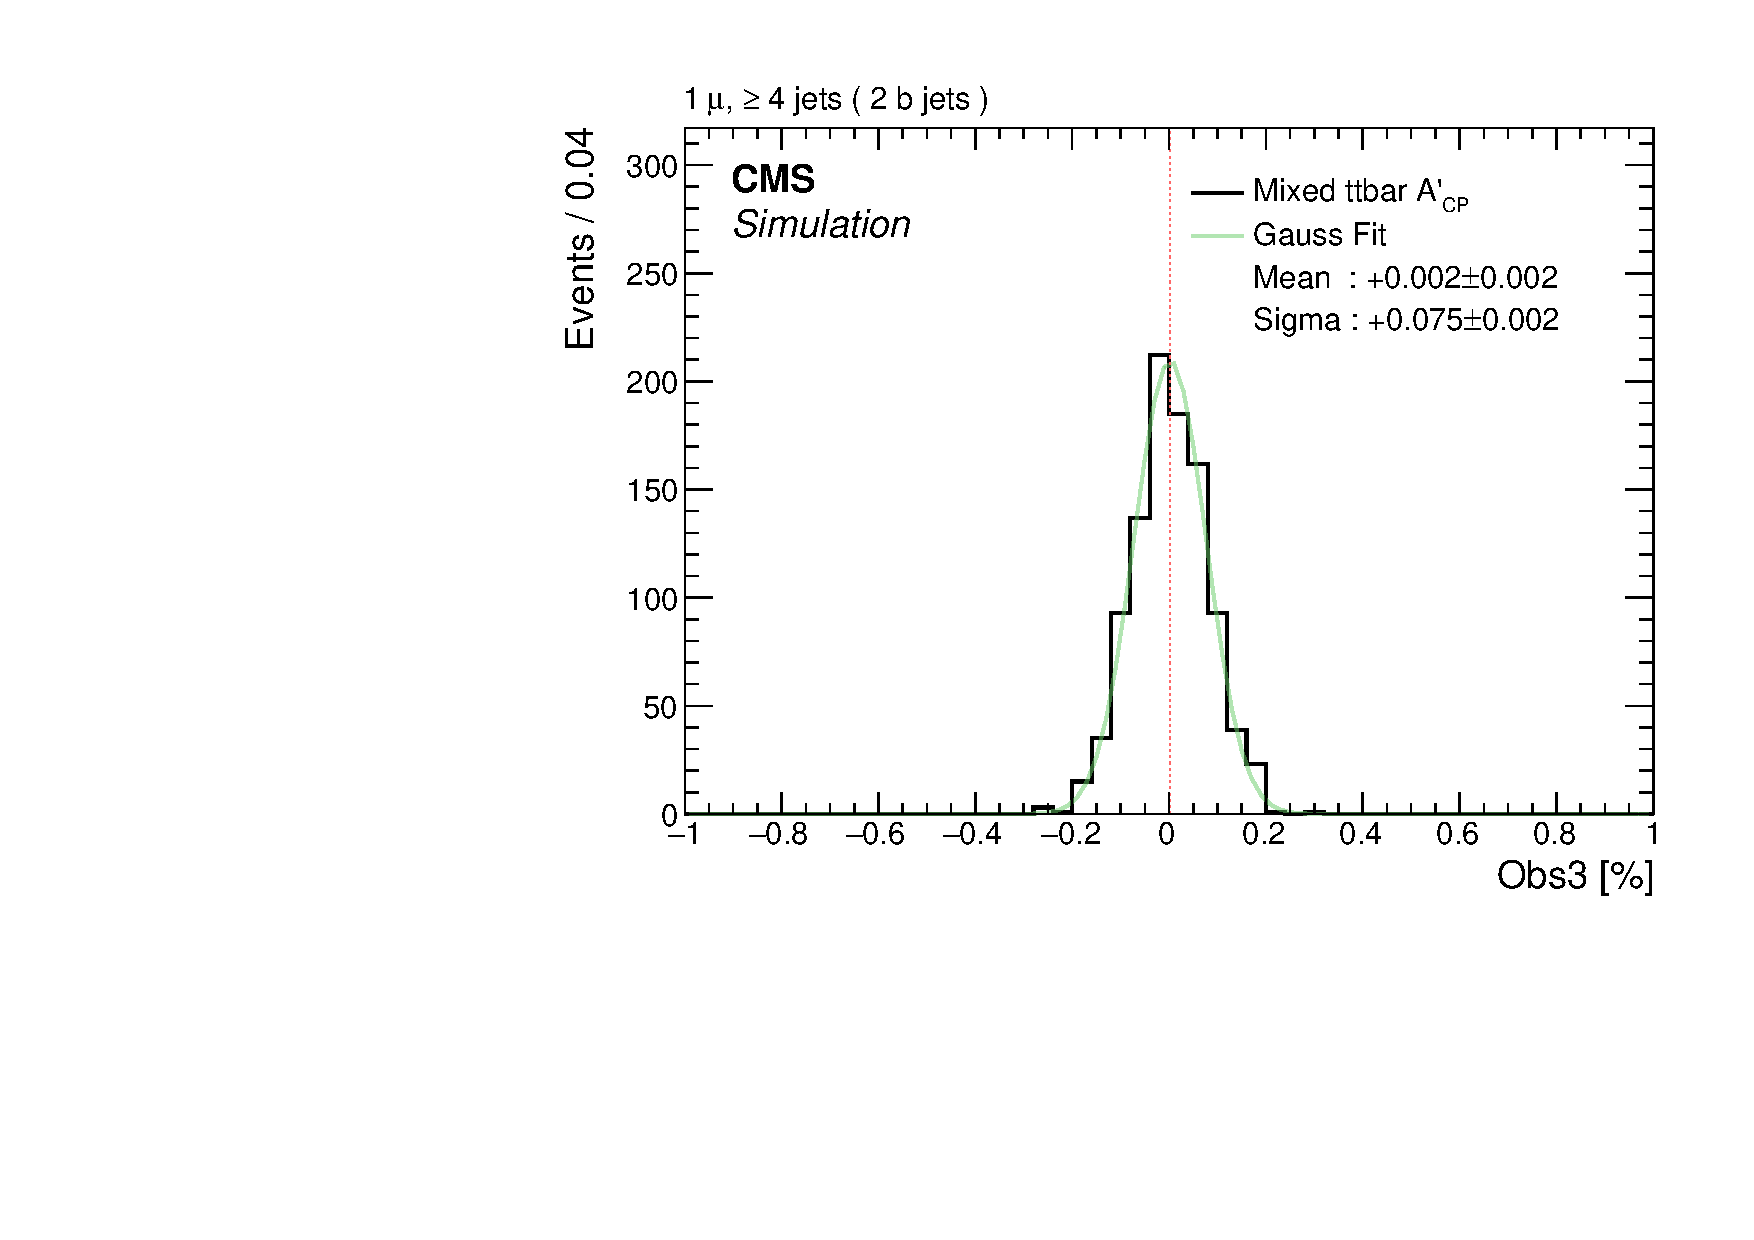
\includegraphics[width=0.45\textwidth]{figure/SimAcp_16_mu_Obs3_Acp_10_mixed.pdf}
    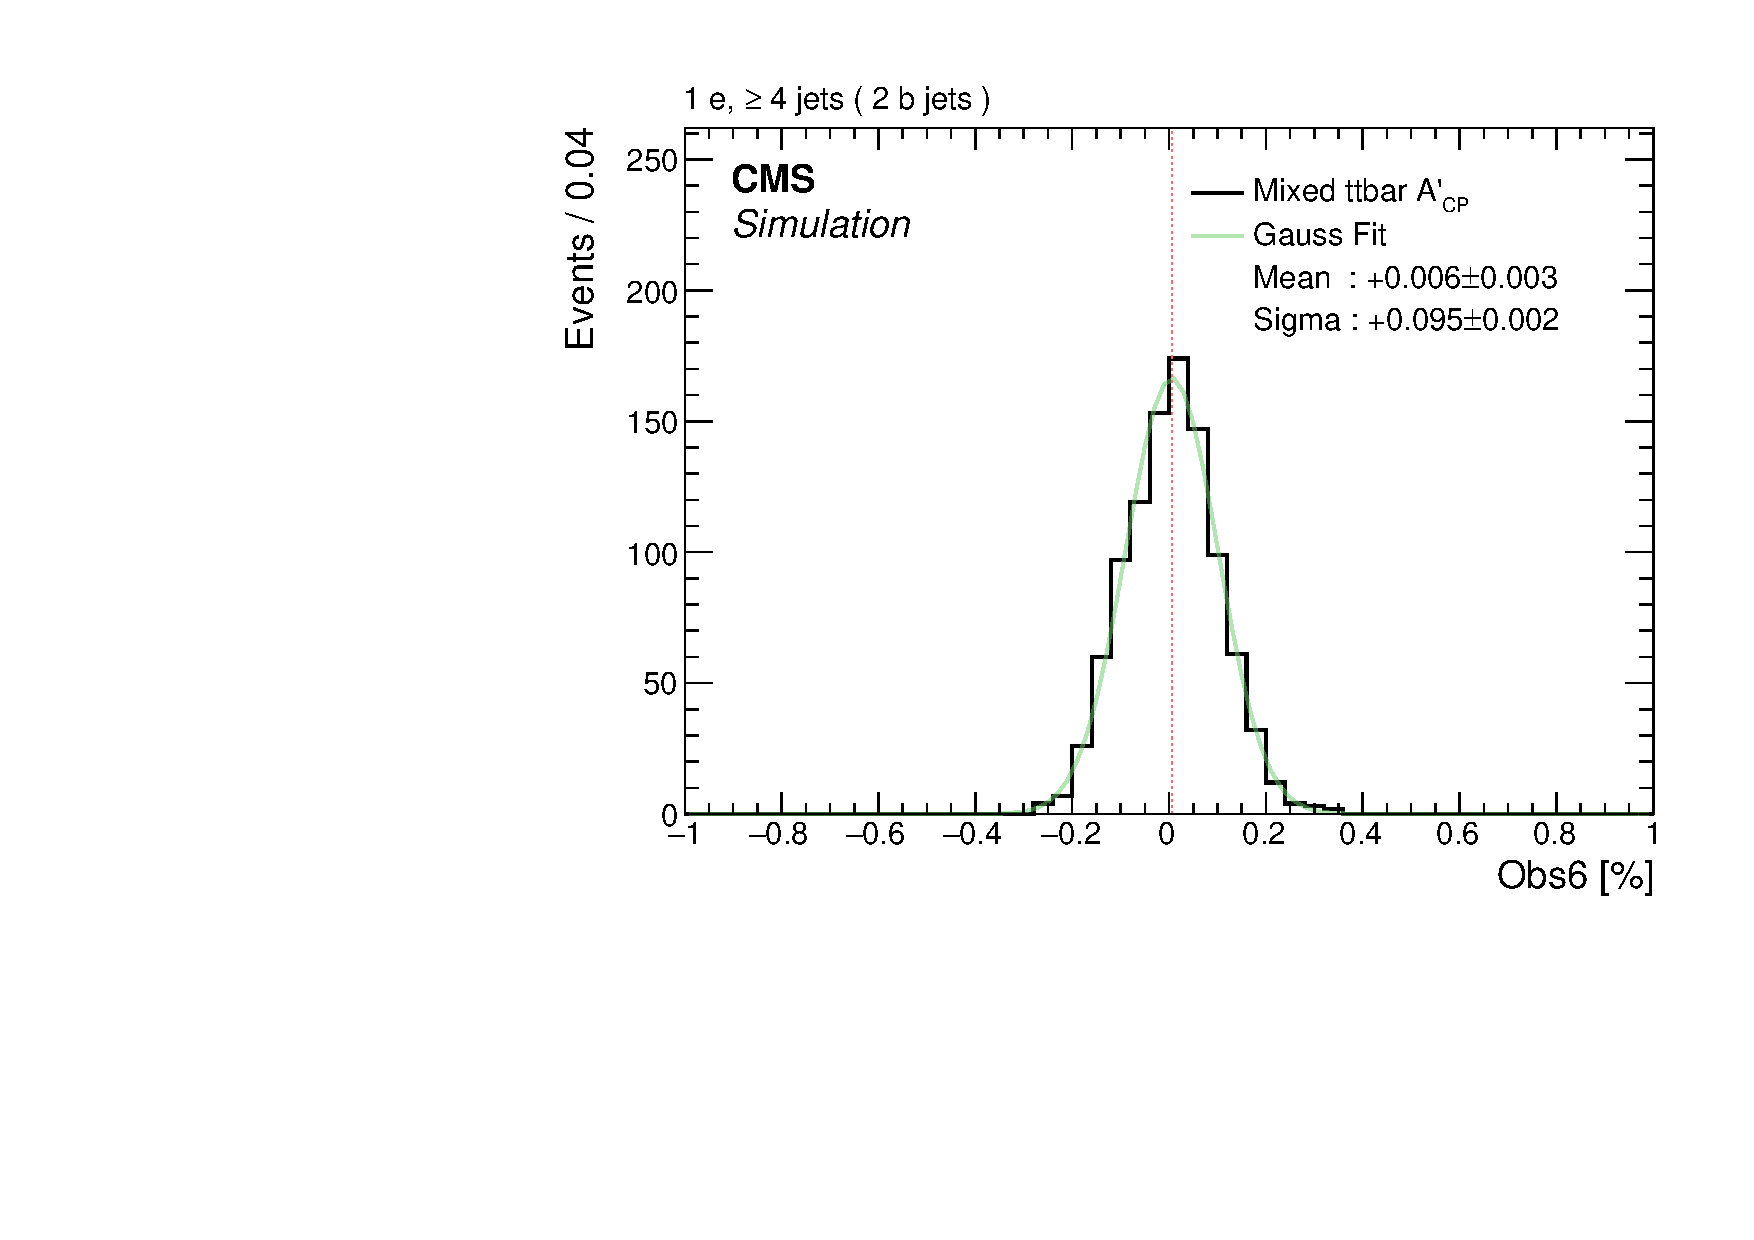
\includegraphics[width=0.45\textwidth]{figure/SimAcp_16_el_Obs6_Acp_10_mixed.pdf}
    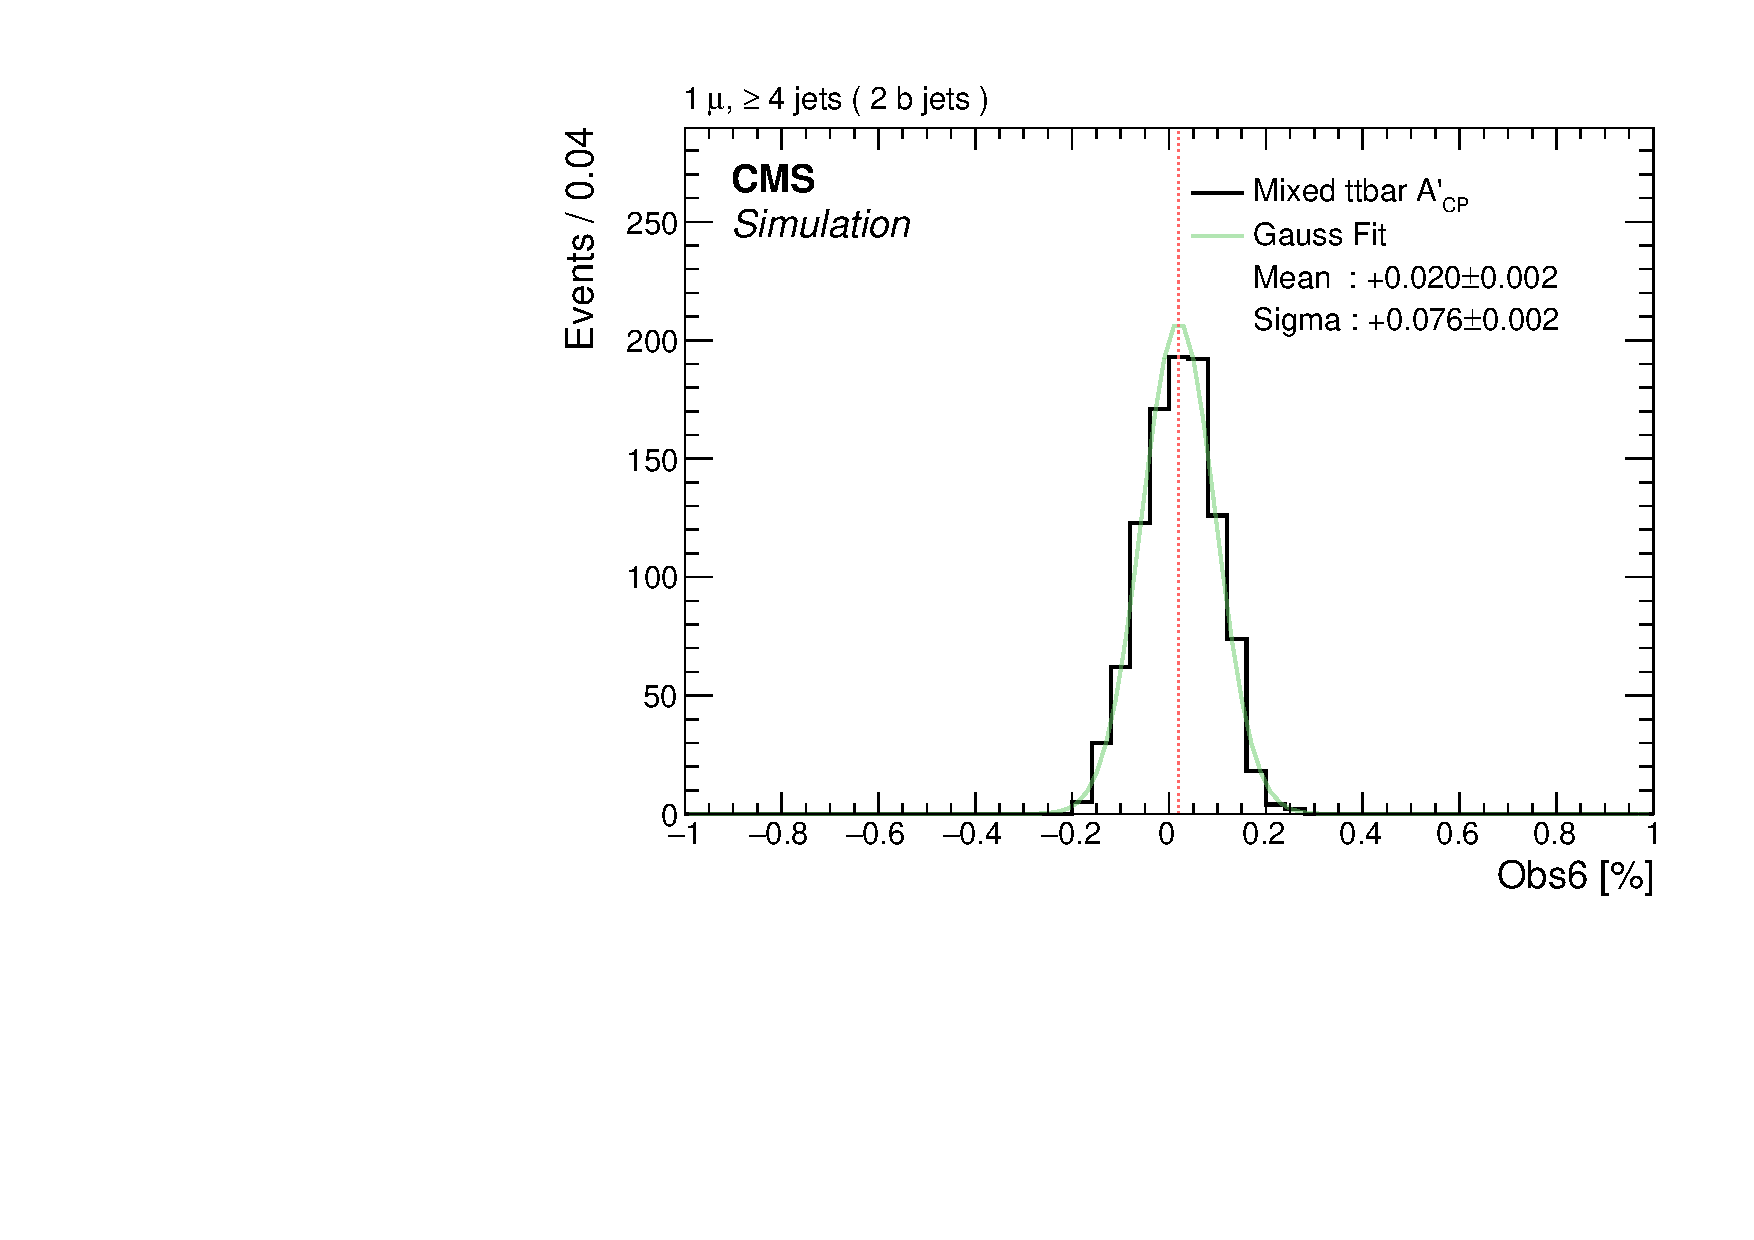
\includegraphics[width=0.45\textwidth]{figure/SimAcp_16_mu_Obs6_Acp_10_mixed.pdf}
    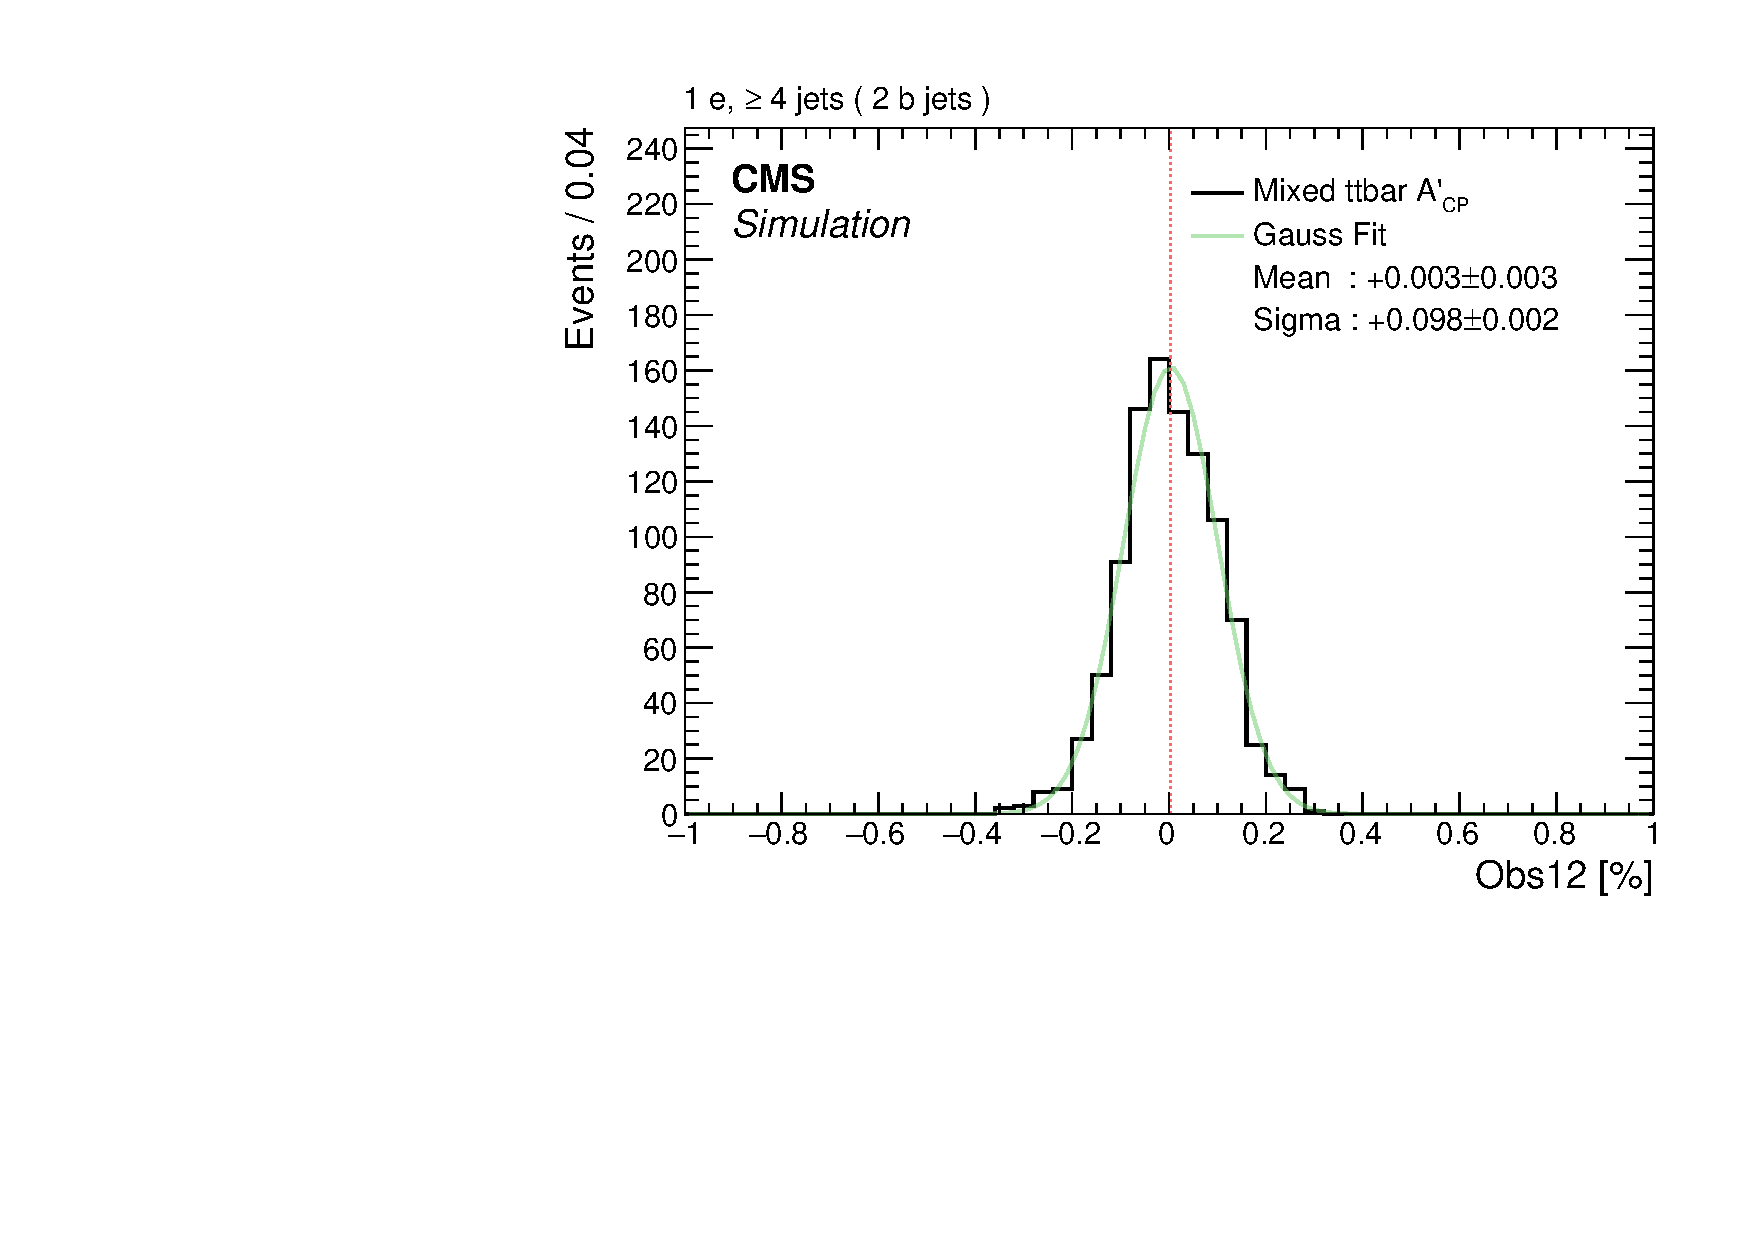
\includegraphics[width=0.45\textwidth]{figure/SimAcp_16_el_Obs12_Acp_10_mixed.pdf}
    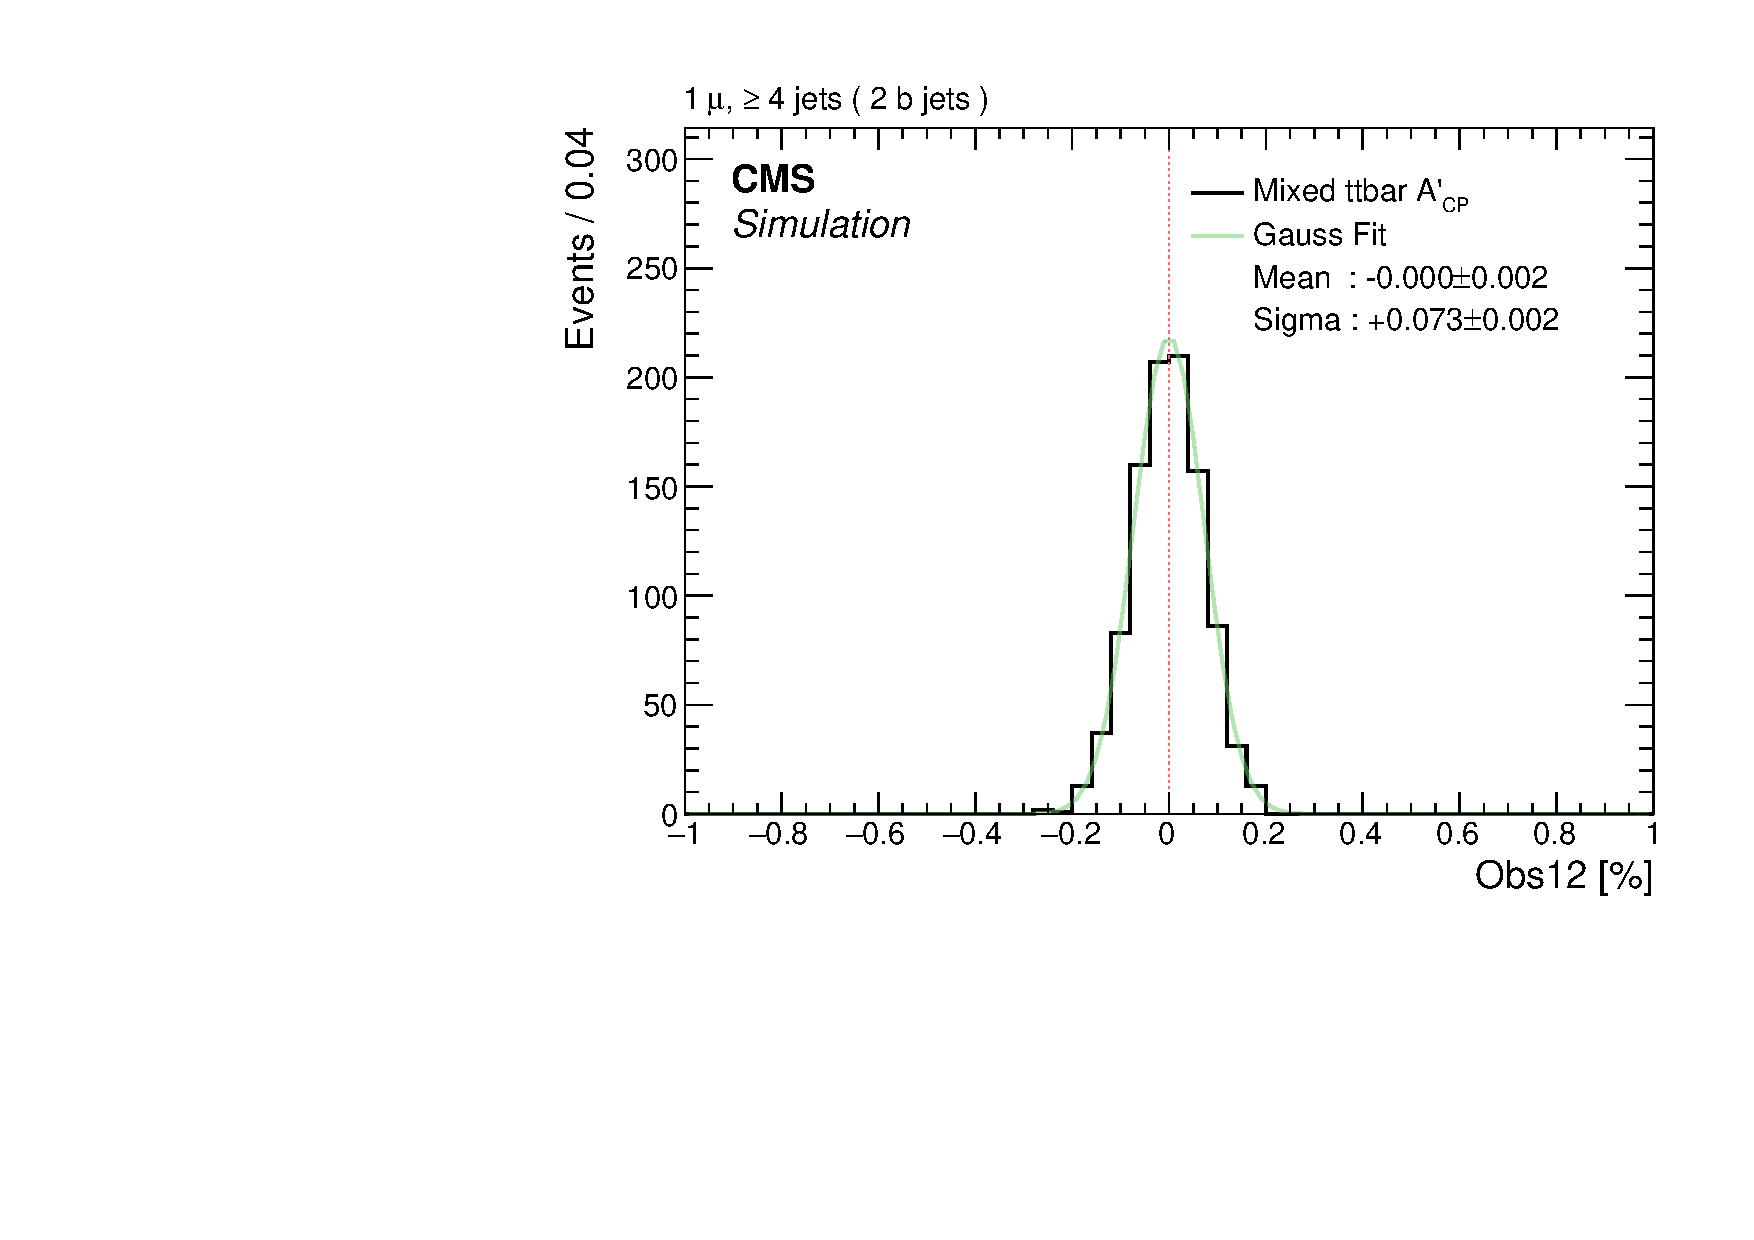
\includegraphics[width=0.45\textwidth]{figure/SimAcp_16_mu_Obs12_Acp_10_mixed.pdf}
    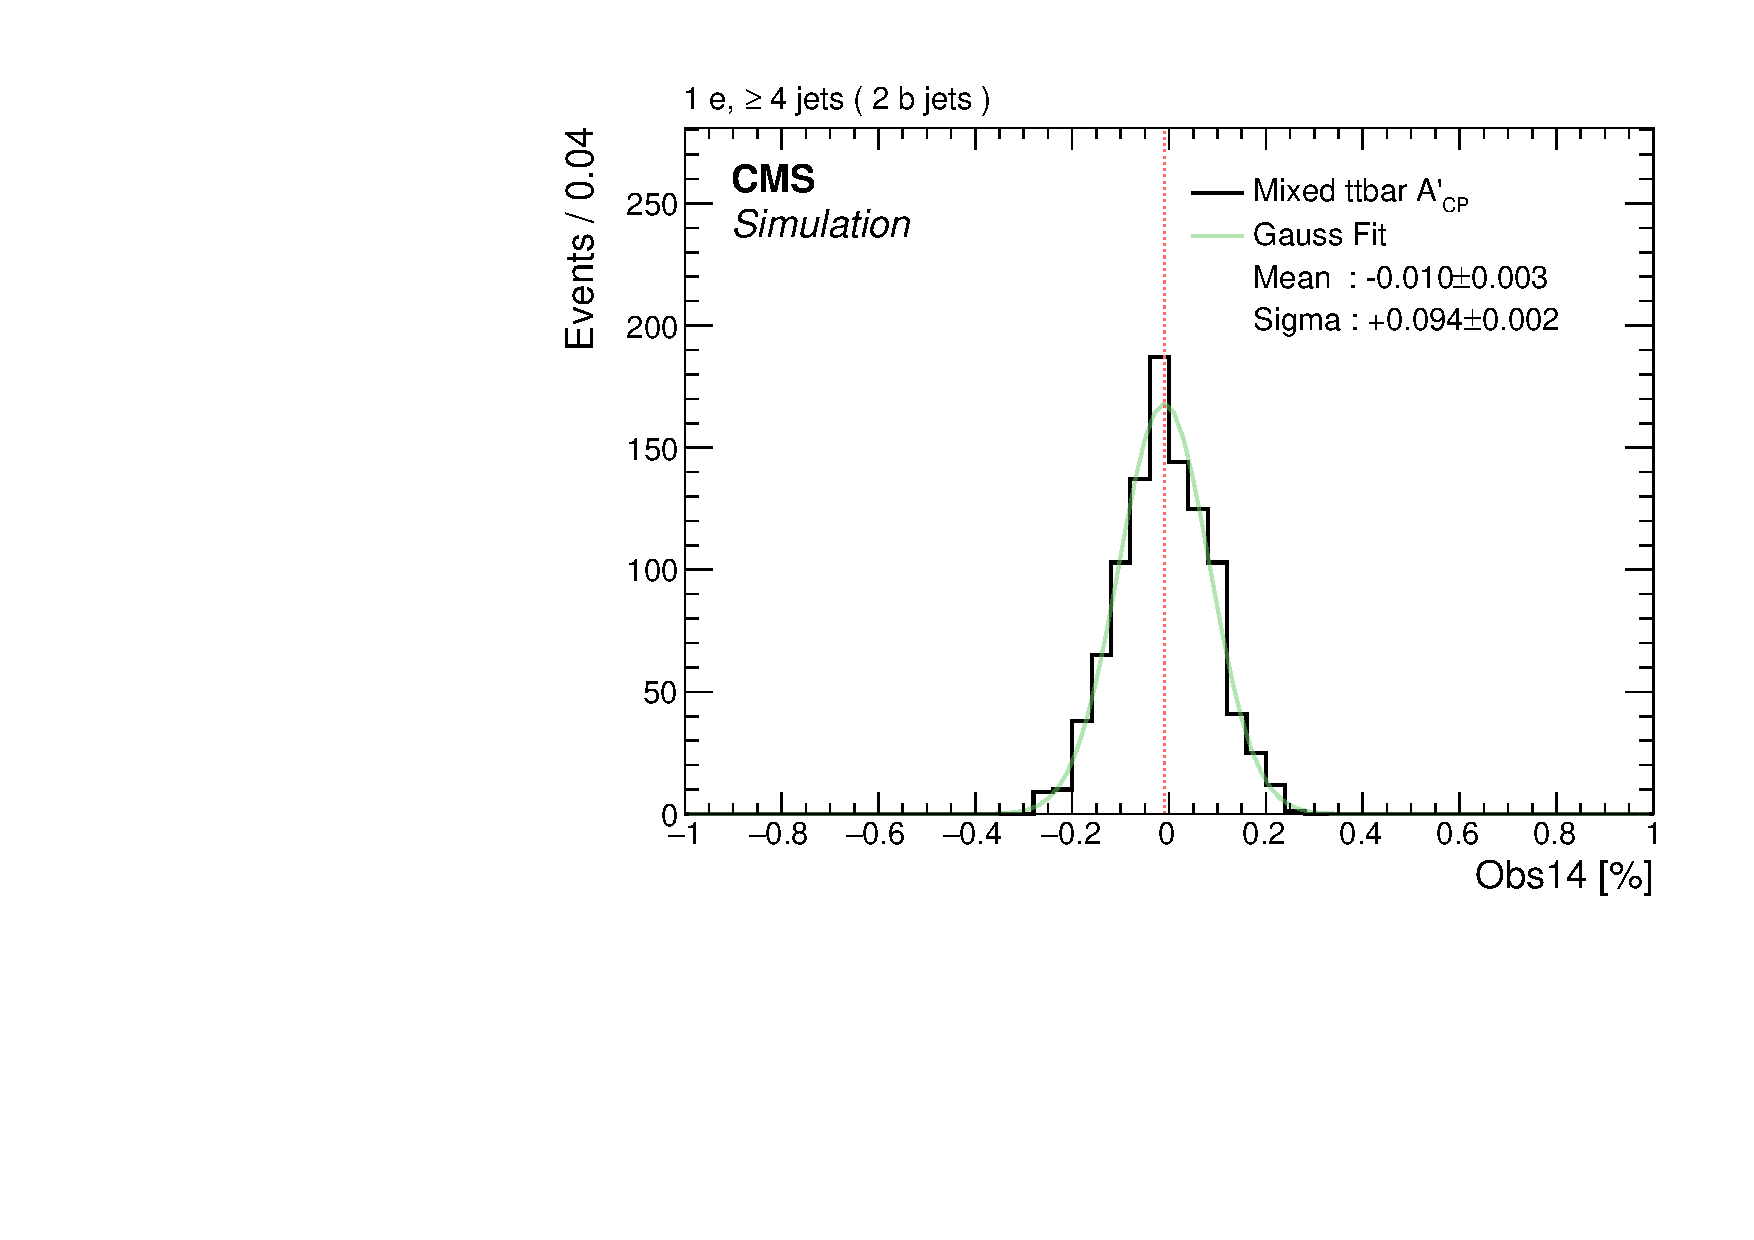
\includegraphics[width=0.45\textwidth]{figure/SimAcp_16_el_Obs14_Acp_10_mixed.pdf}
    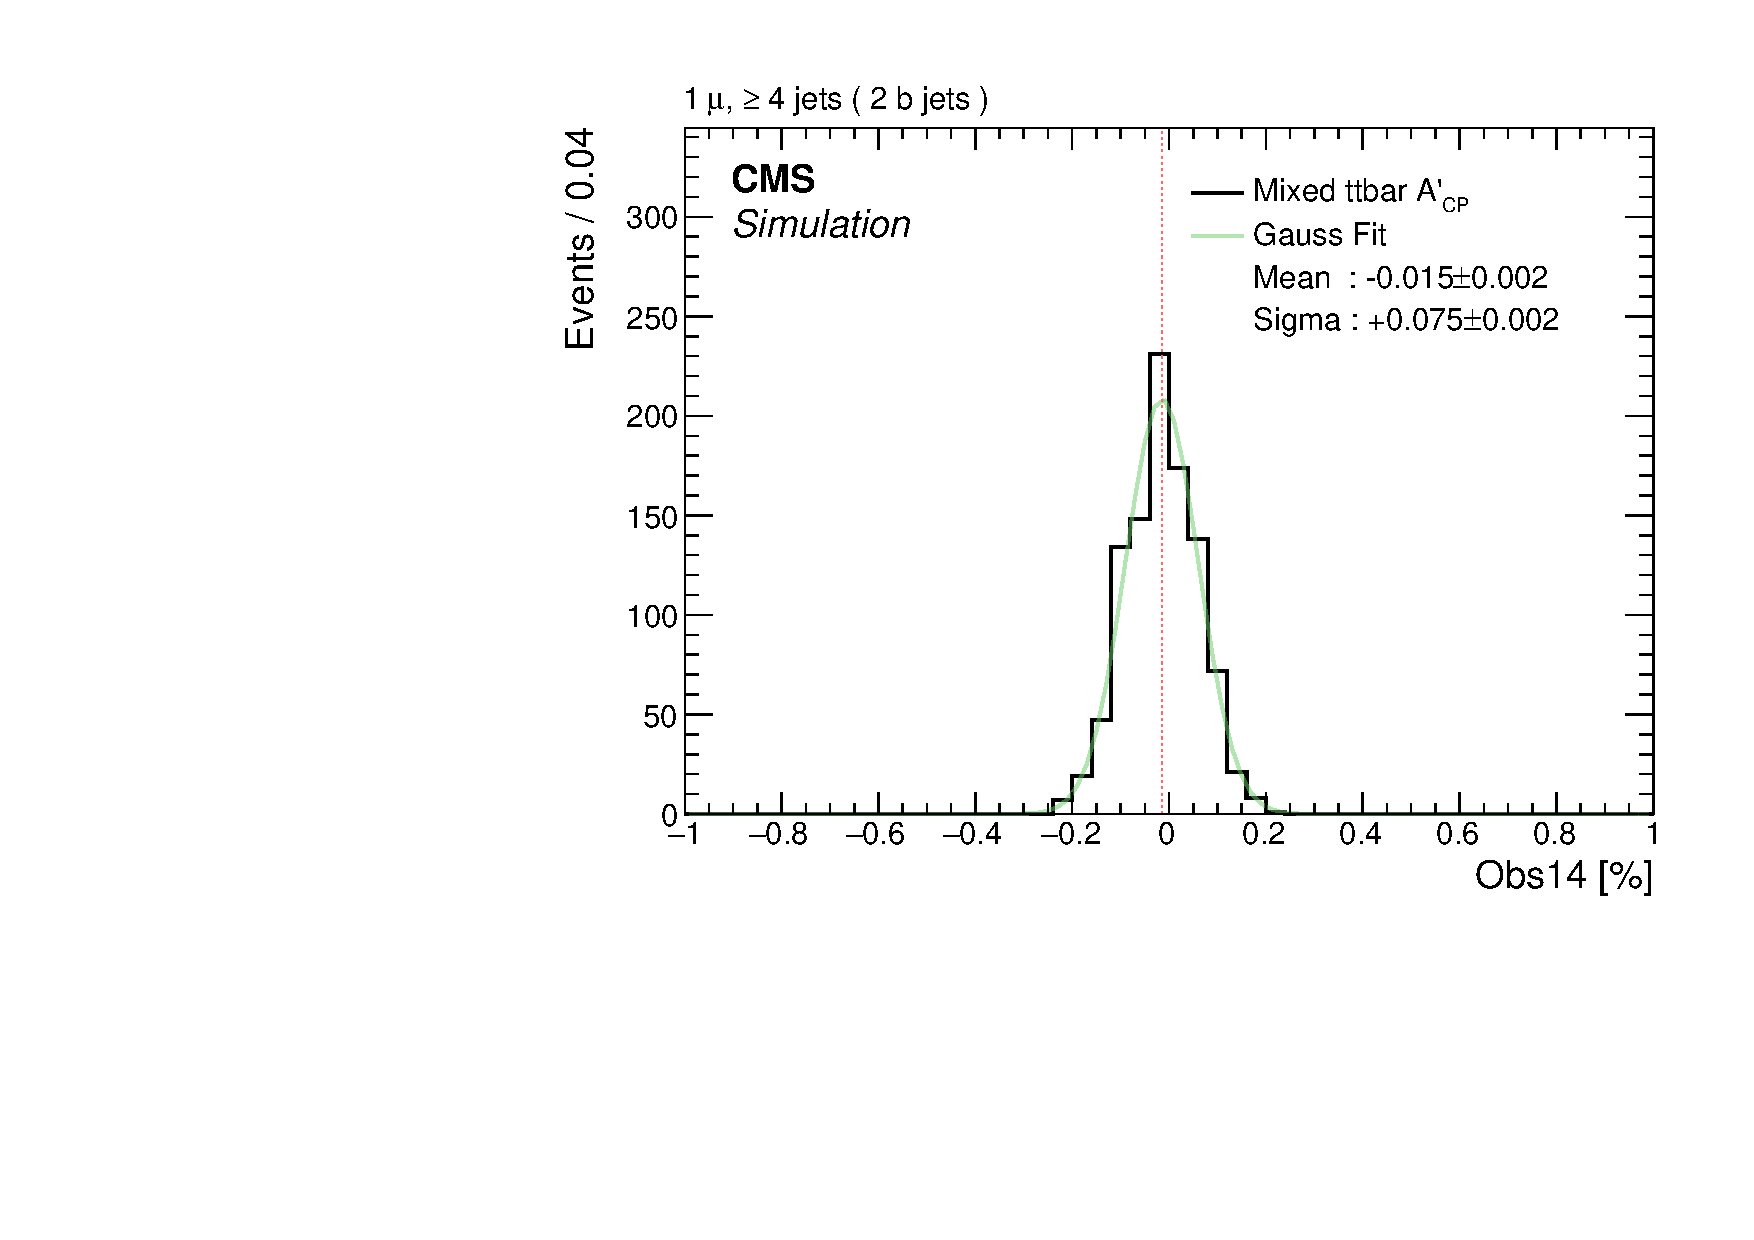
\includegraphics[width=0.45\textwidth]{figure/SimAcp_16_mu_Obs14_Acp_10_mixed.pdf}
    \caption[The \Acpprime distribution after applying the event-mixing method to \ttbar events in 2016 samples.]
    {
        The \Acpprime distribution after applying the event-mixing method to \ttbar events with artificial \Acpprime in 2016 samples. 
        The green line is the fitted gaussian and the red dotted line presents the mean value of the gaussian.
        The electron channel is on the left, and the muon channel is on the right.
    }
    \label{fig:16_exchanging_simulation_acp}
\end{figure}
\begin{figure}
    \centering
    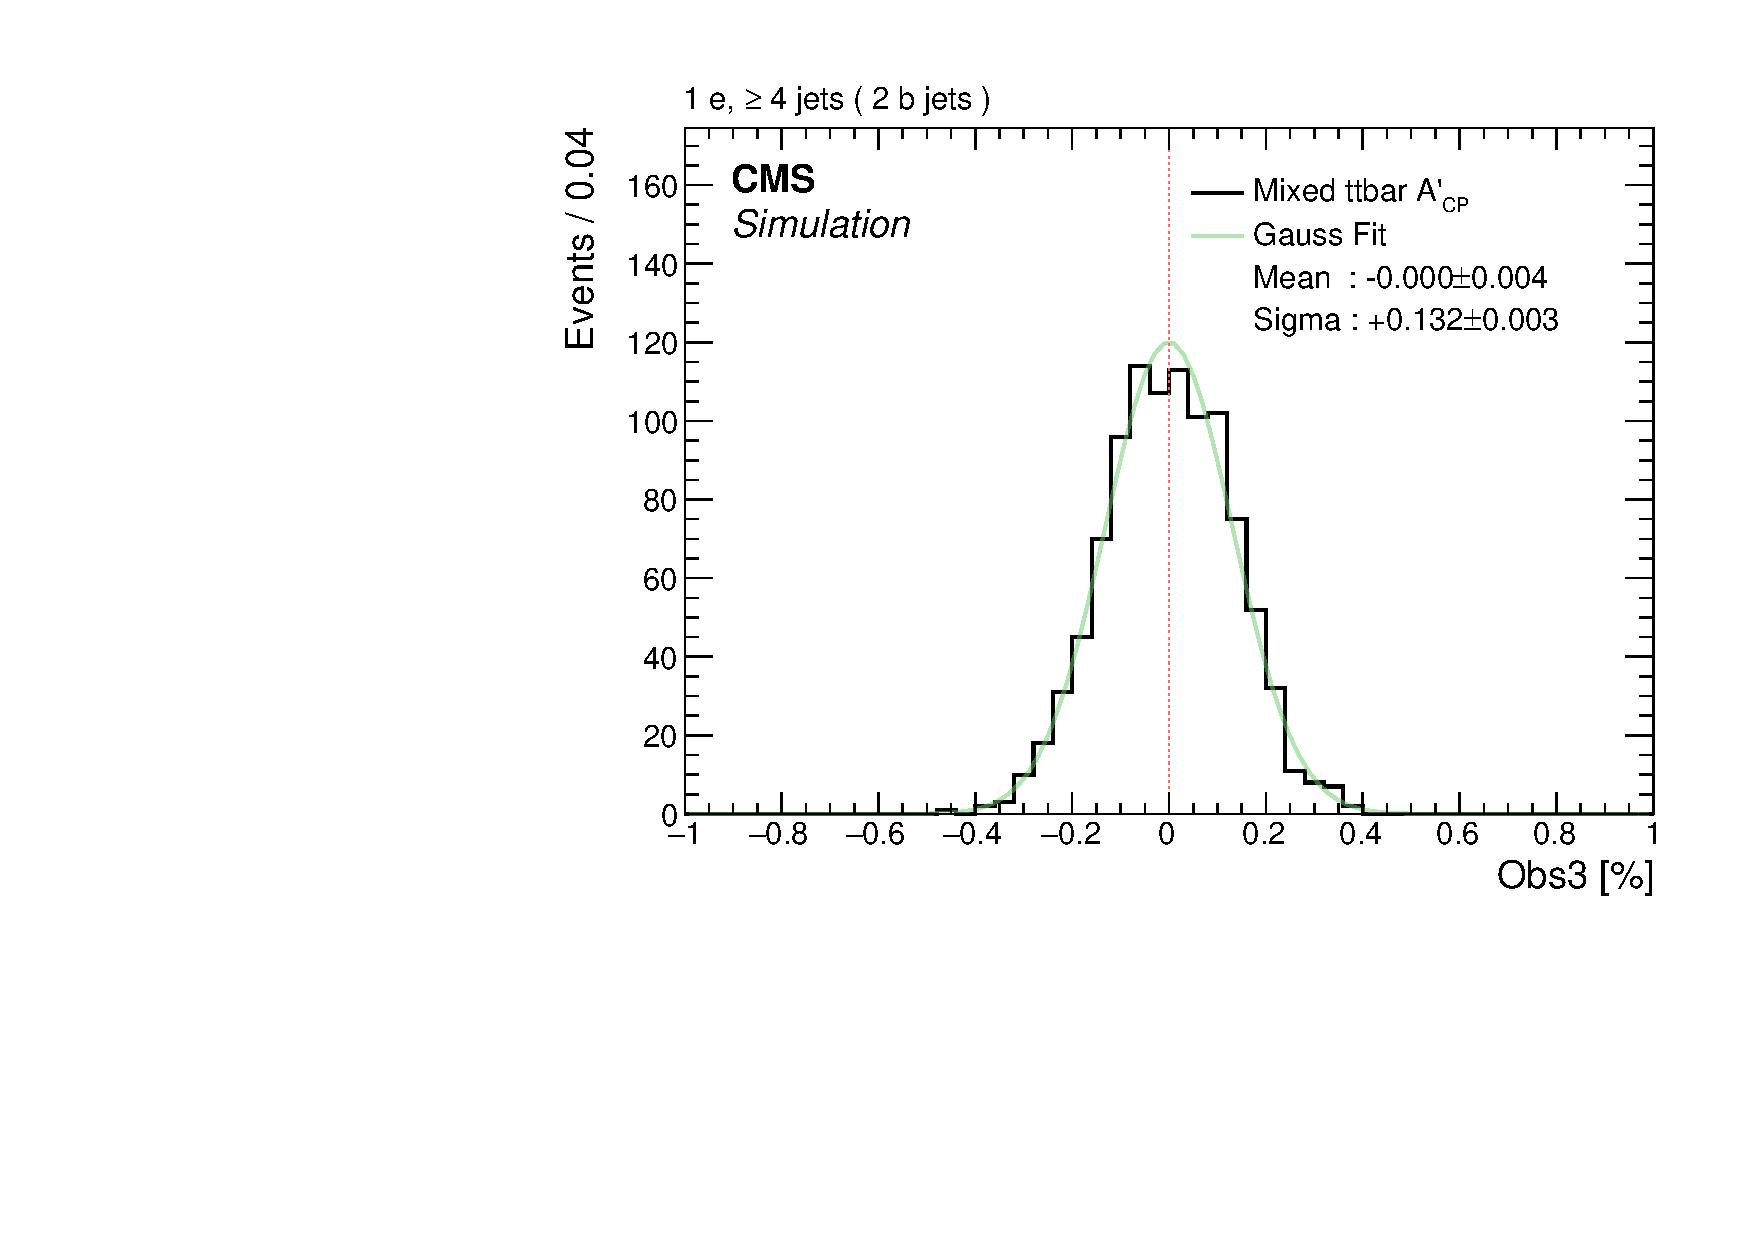
\includegraphics[width=0.45\textwidth]{figure/SimAcp_17_el_Obs3_Acp_10_mixed.pdf}
    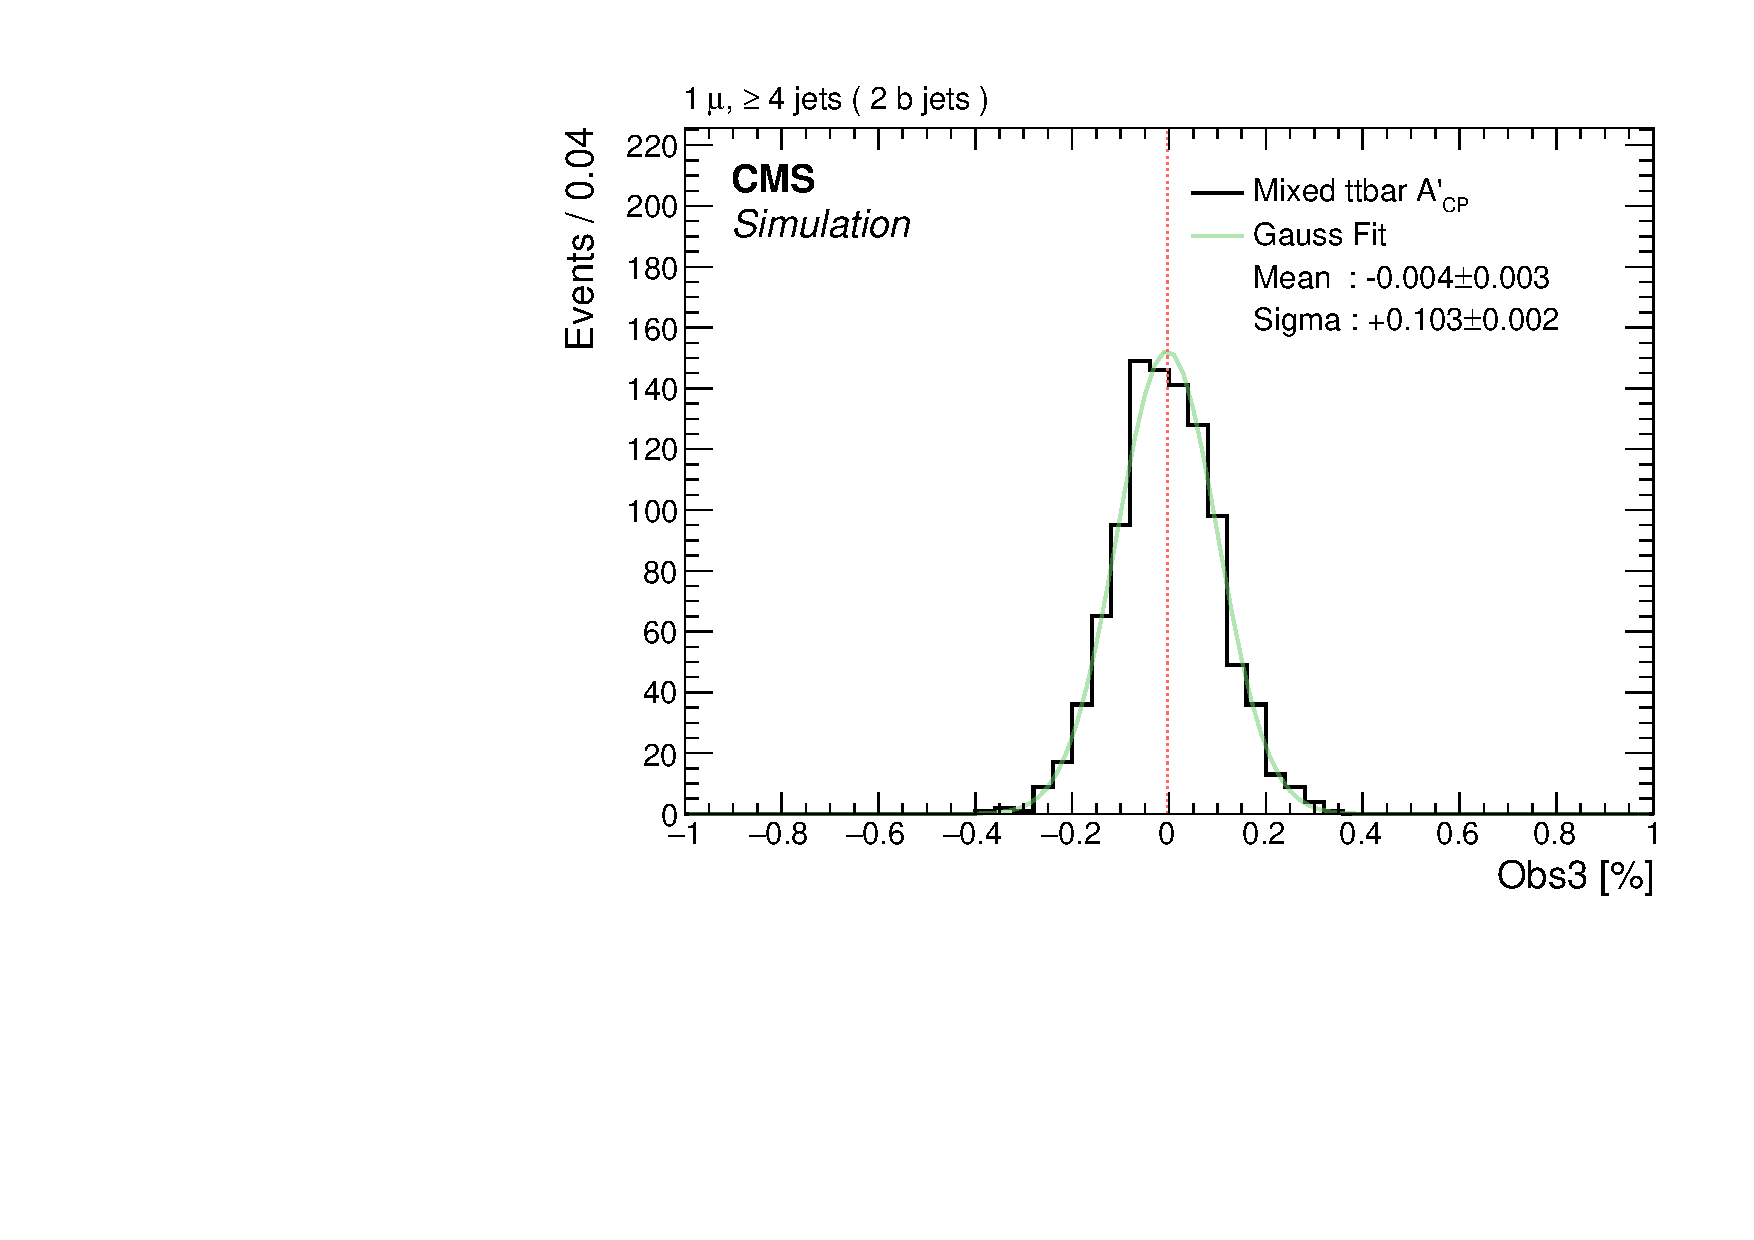
\includegraphics[width=0.45\textwidth]{figure/SimAcp_17_mu_Obs3_Acp_10_mixed.pdf}
    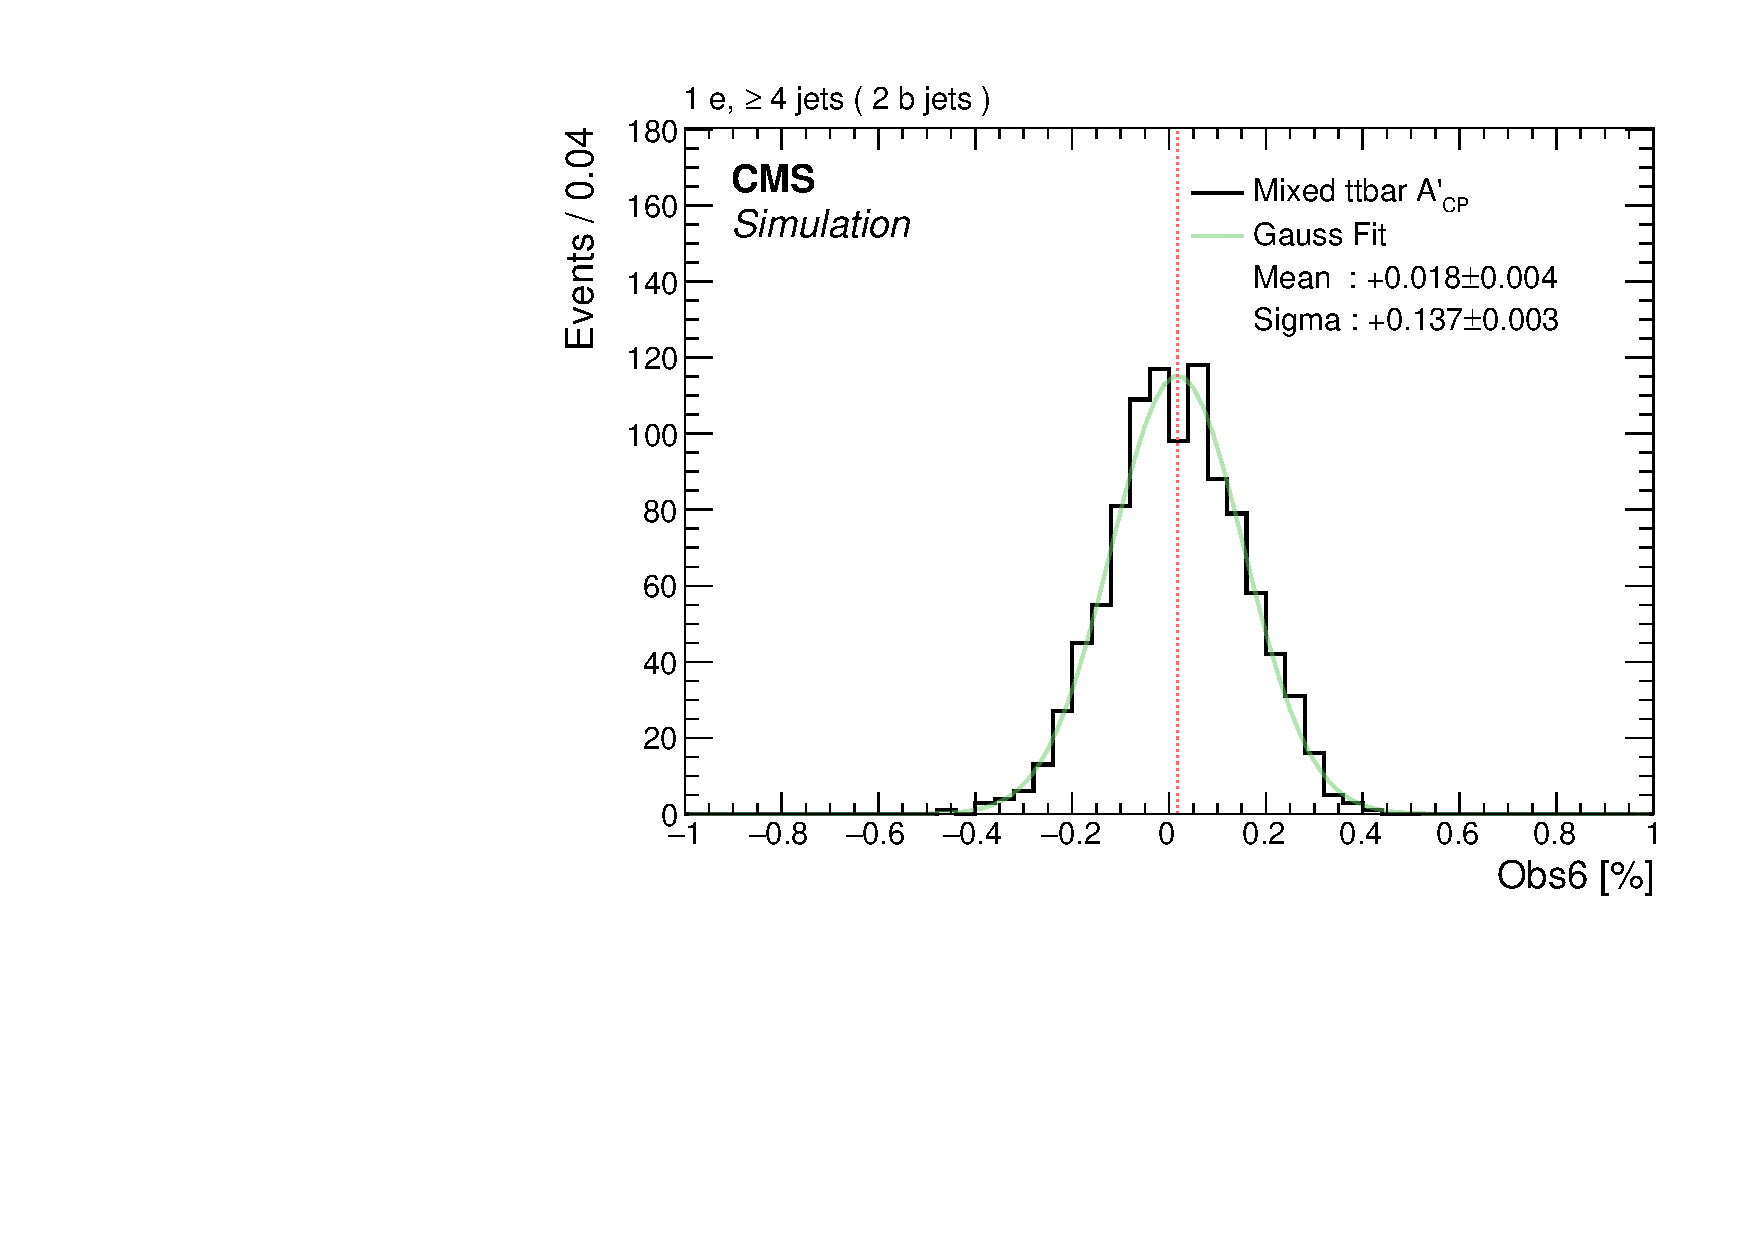
\includegraphics[width=0.45\textwidth]{figure/SimAcp_17_el_Obs6_Acp_10_mixed.pdf}
    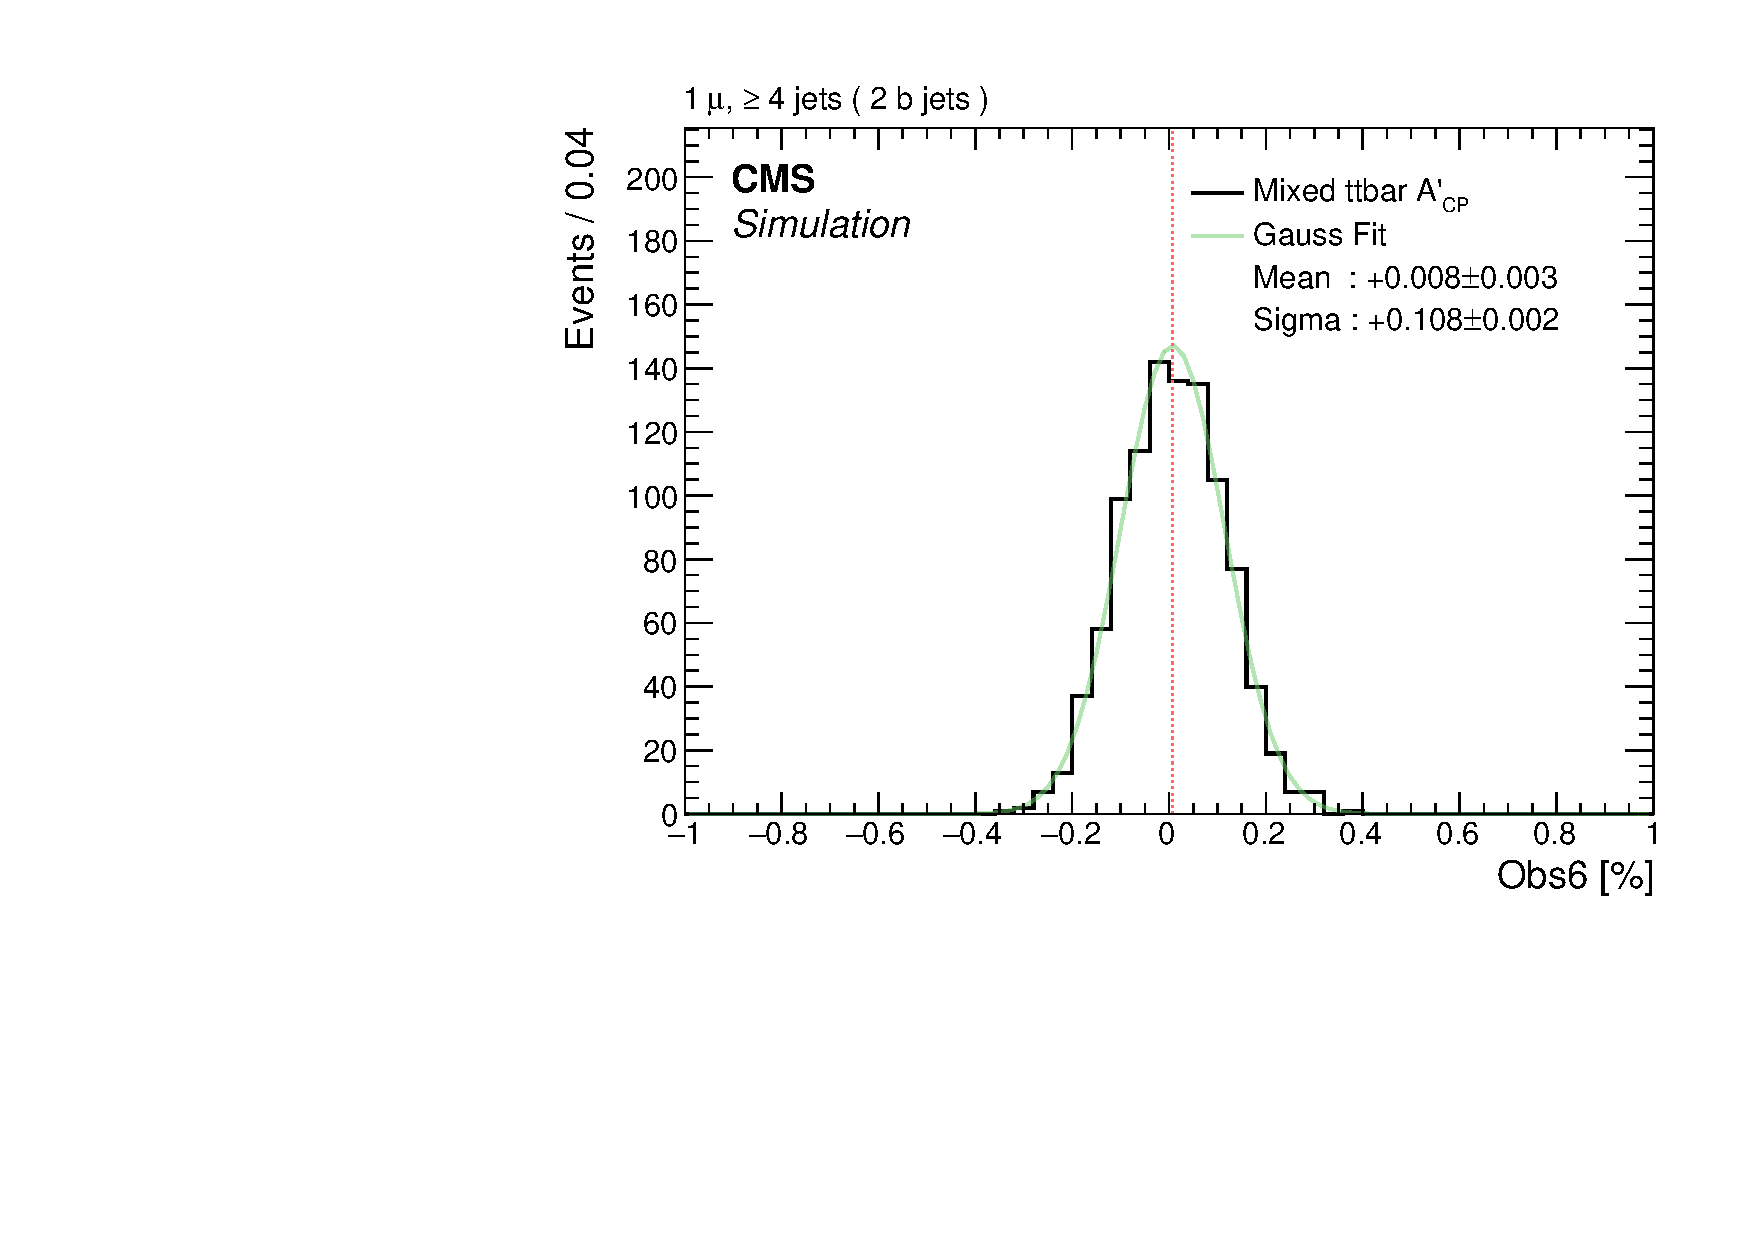
\includegraphics[width=0.45\textwidth]{figure/SimAcp_17_mu_Obs6_Acp_10_mixed.pdf}
    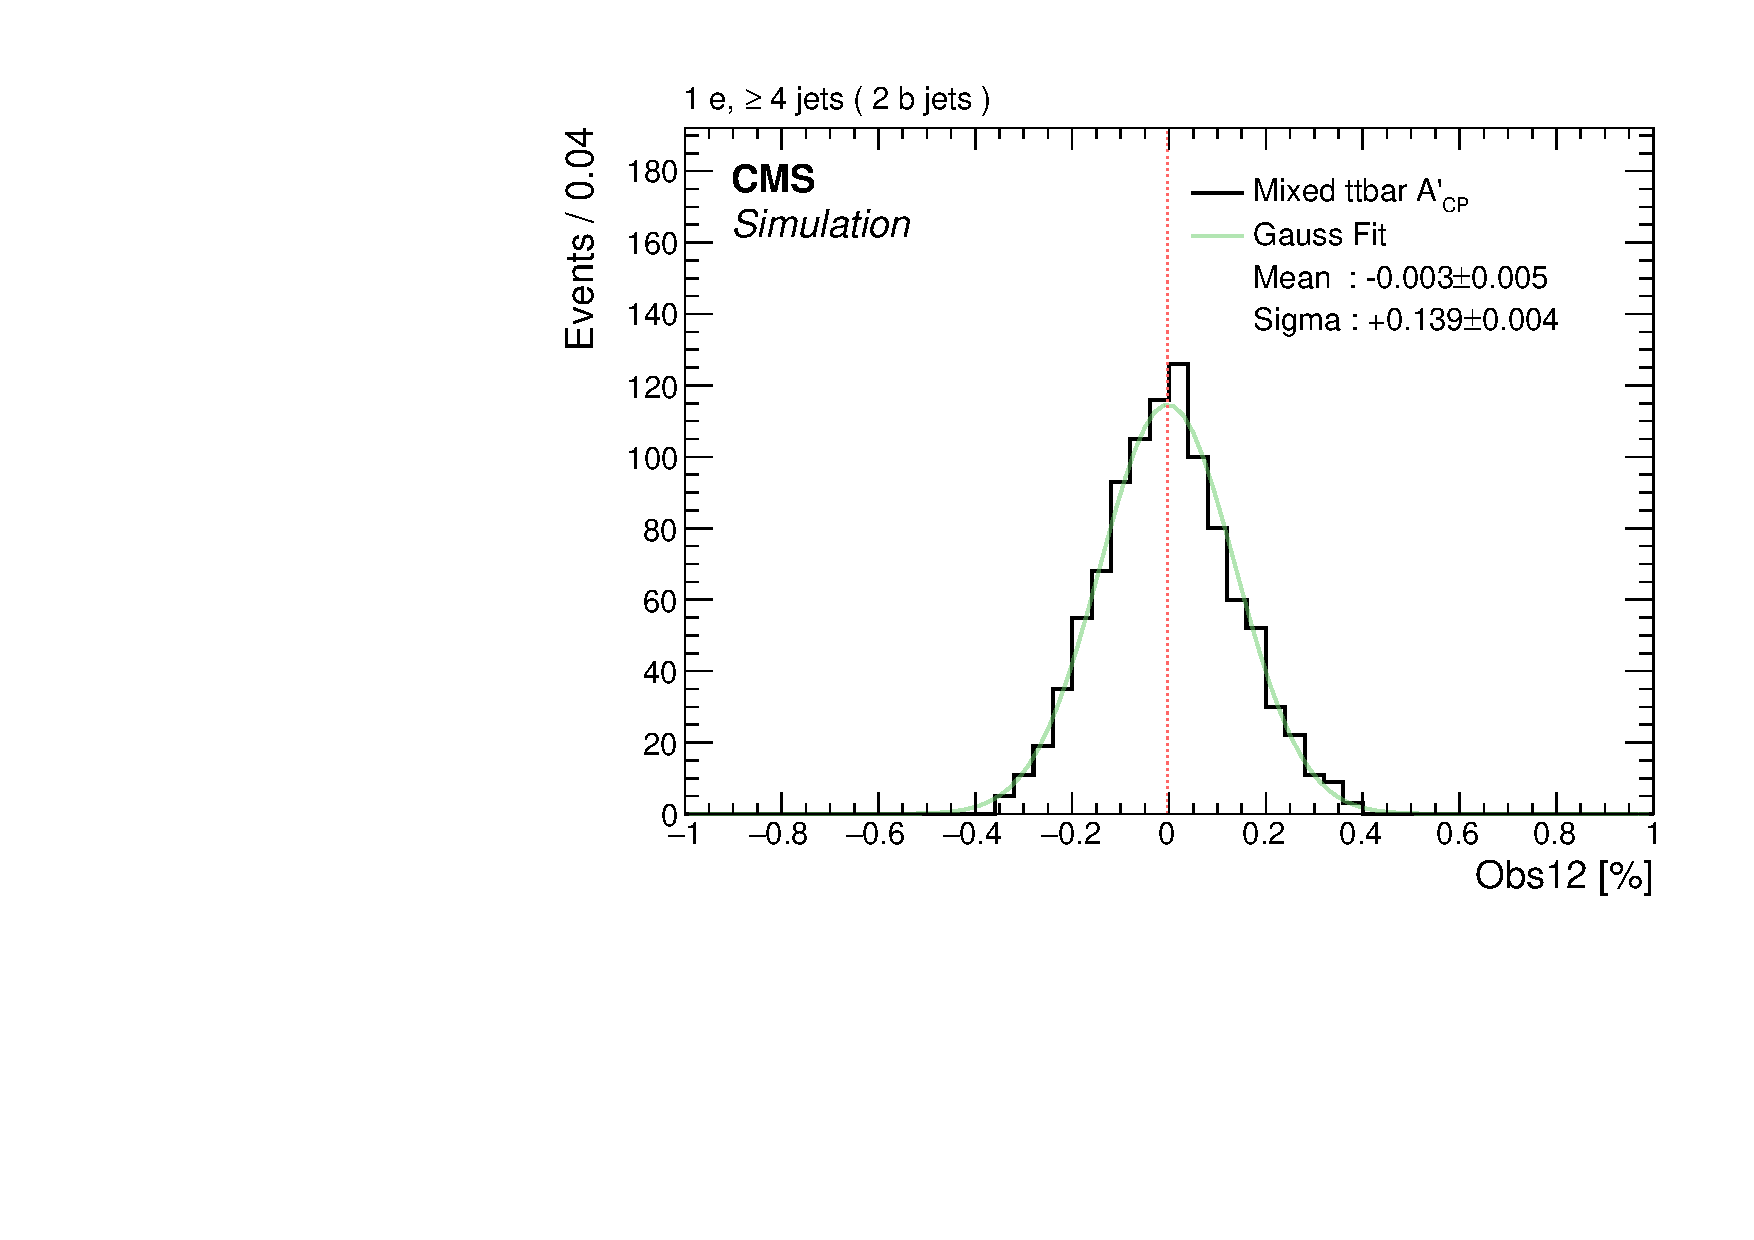
\includegraphics[width=0.45\textwidth]{figure/SimAcp_17_el_Obs12_Acp_10_mixed.pdf}
    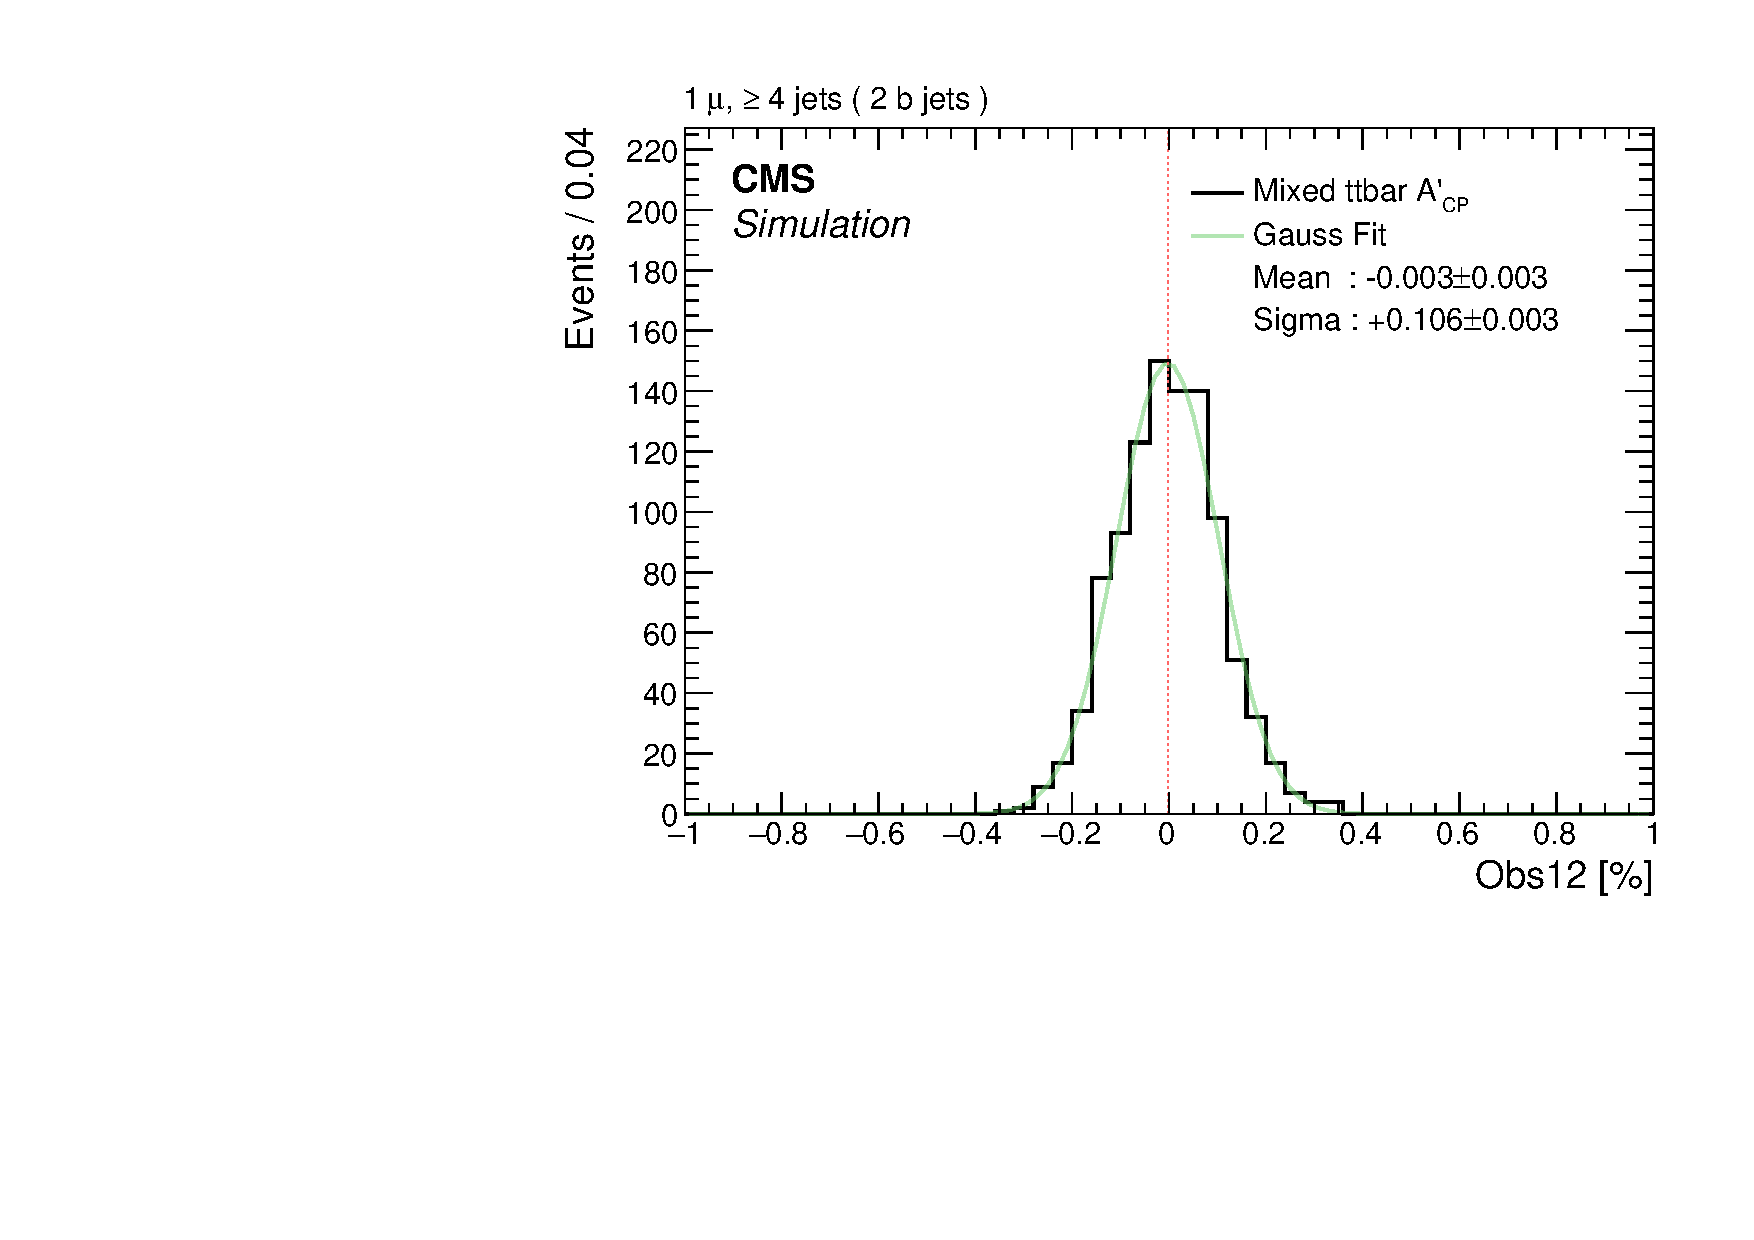
\includegraphics[width=0.45\textwidth]{figure/SimAcp_17_mu_Obs12_Acp_10_mixed.pdf}
    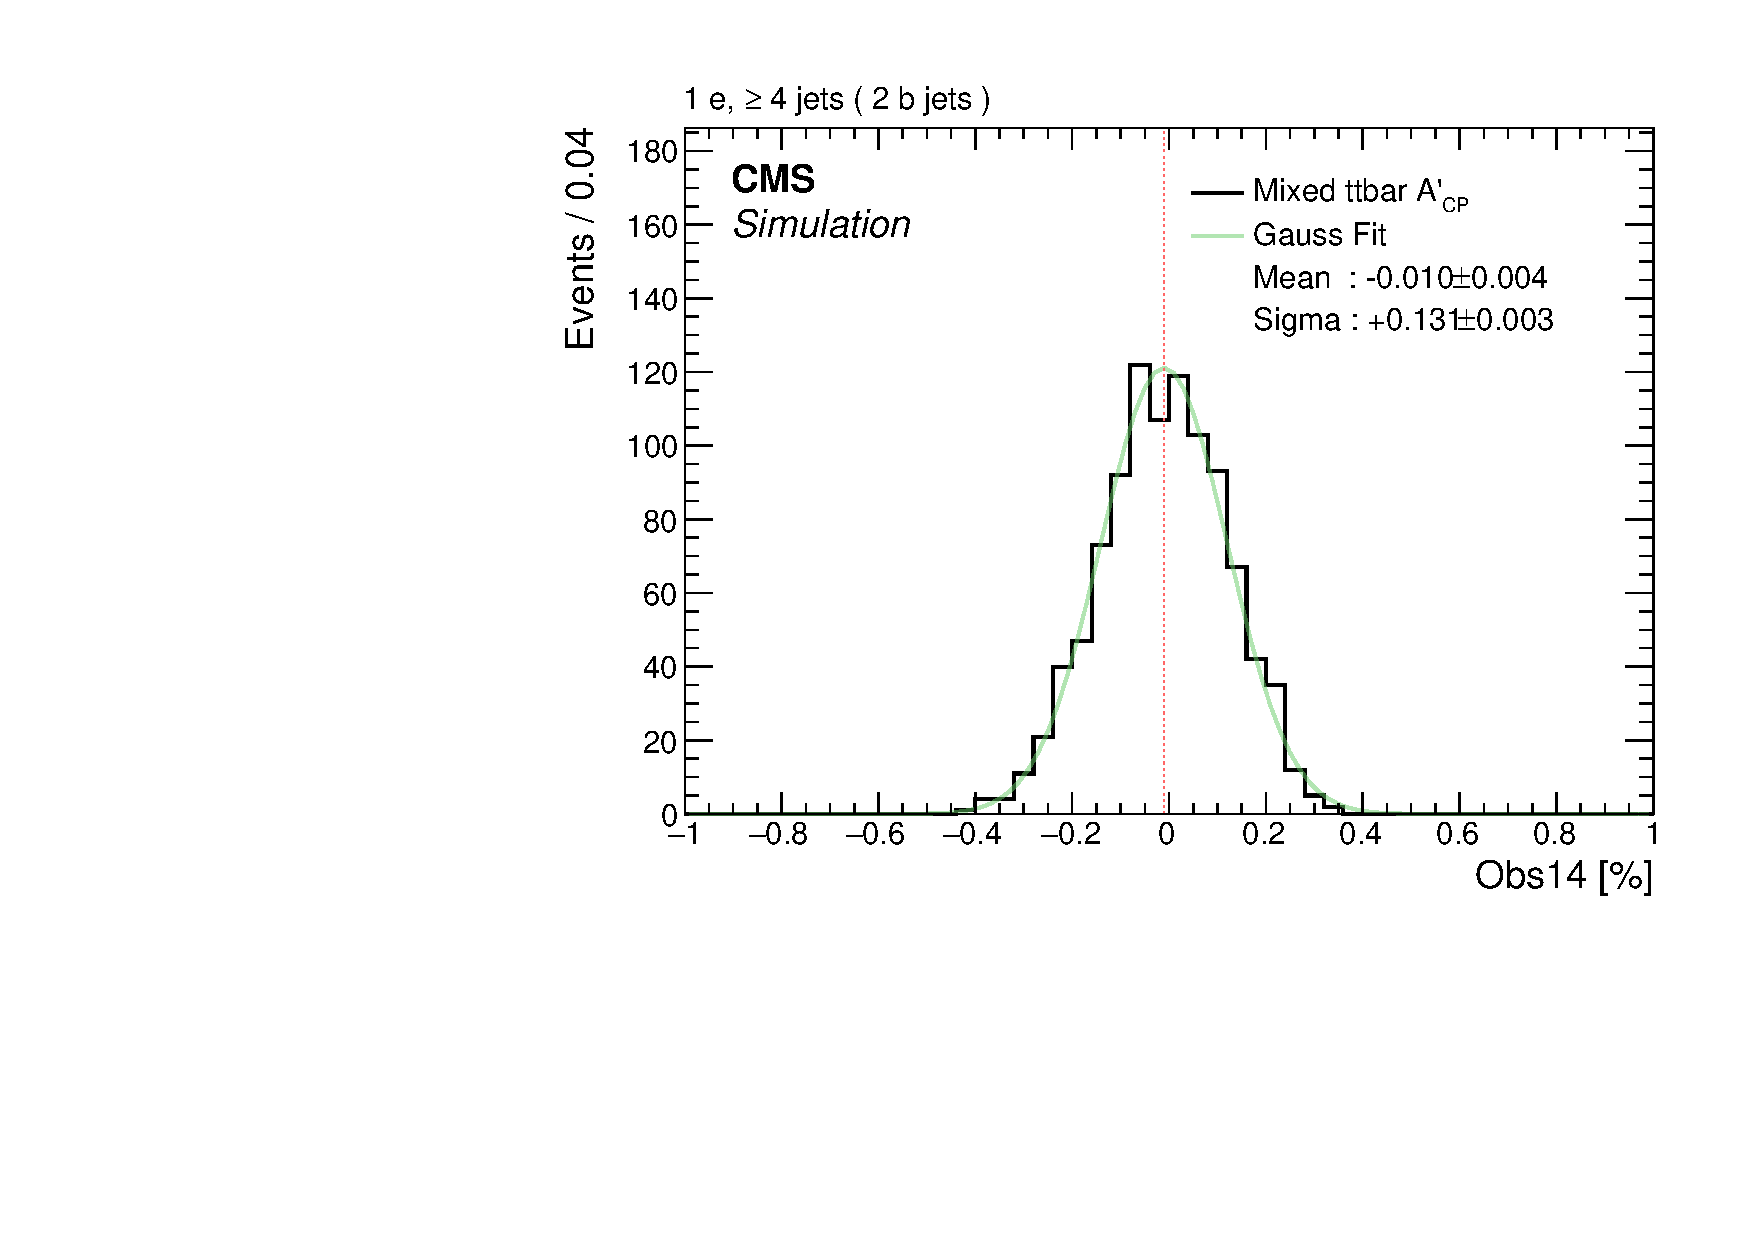
\includegraphics[width=0.45\textwidth]{figure/SimAcp_17_el_Obs14_Acp_10_mixed.pdf}
    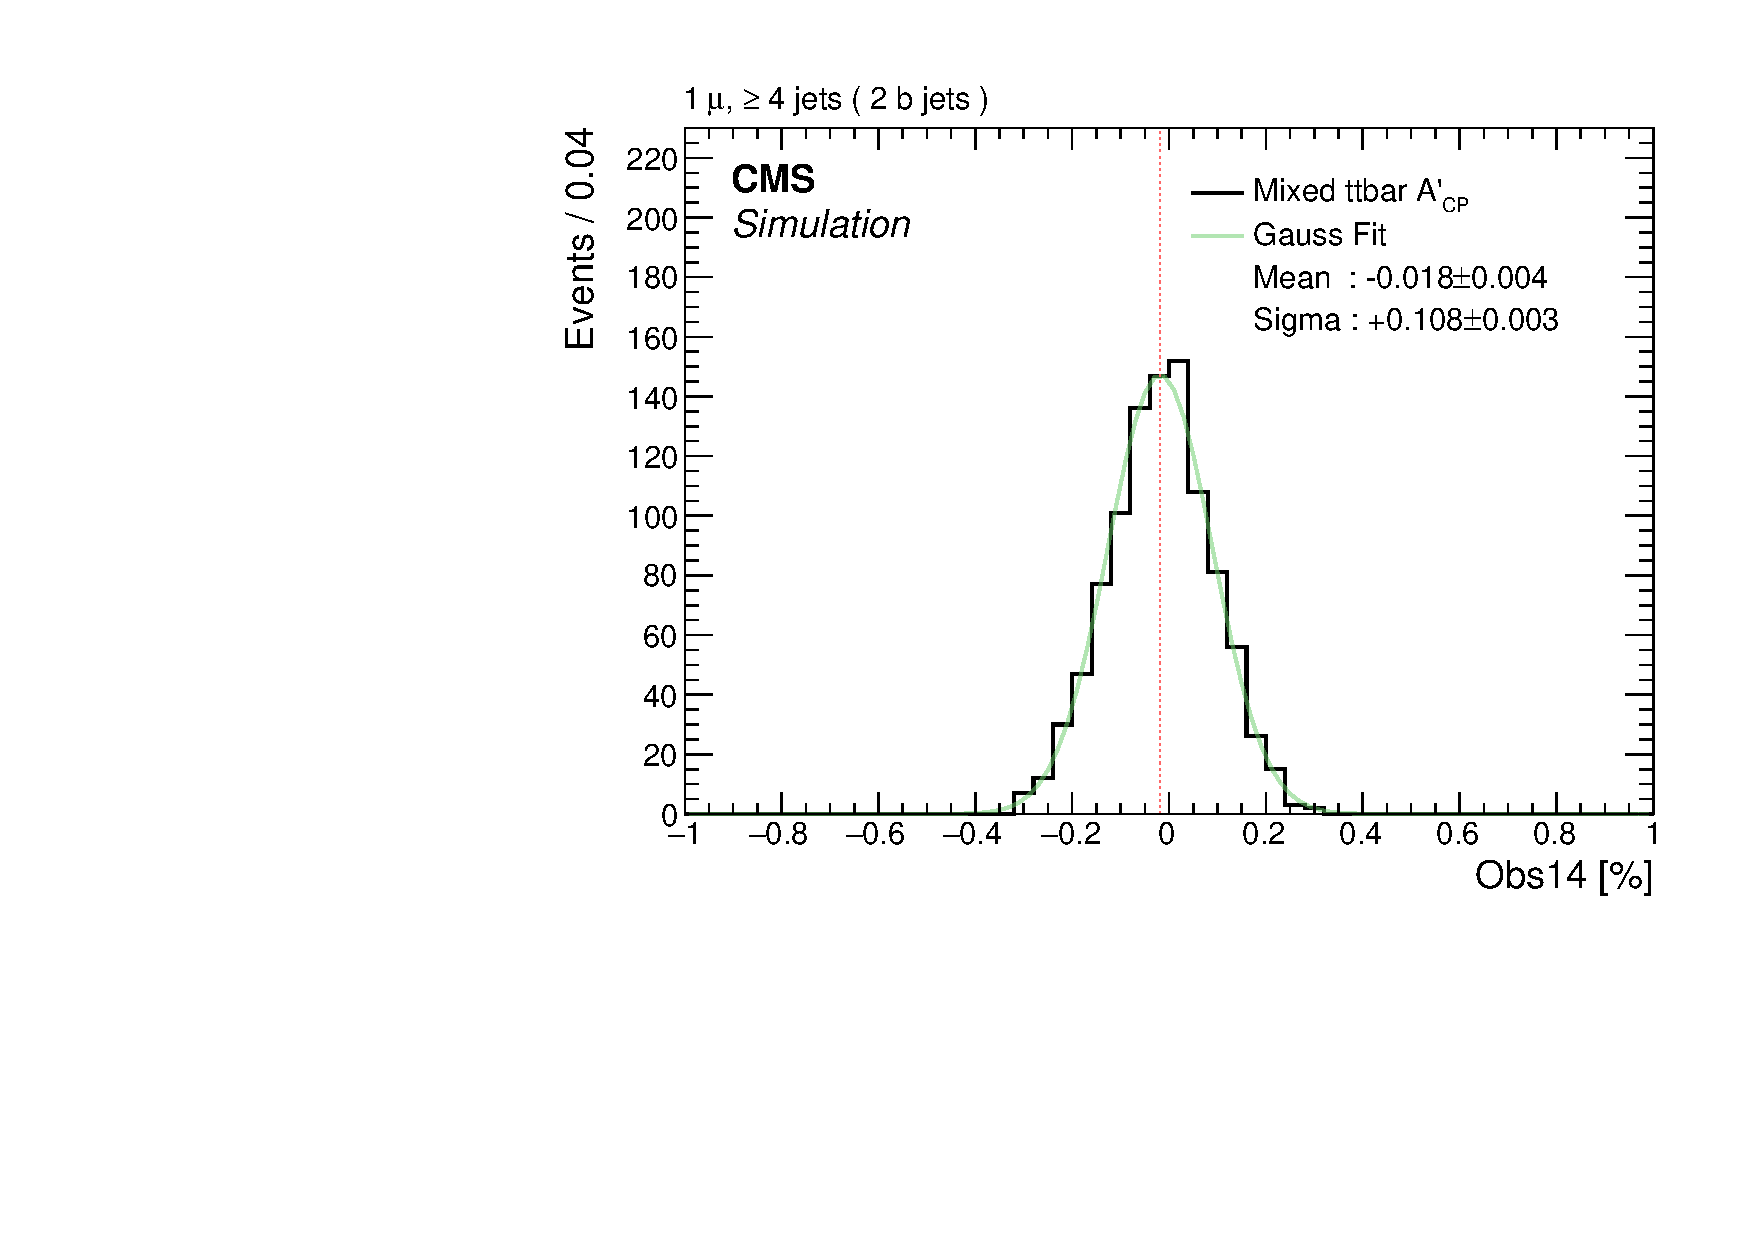
\includegraphics[width=0.45\textwidth]{figure/SimAcp_17_mu_Obs14_Acp_10_mixed.pdf}
    \caption[The \Acpprime distribution after applying the event-mixing method to \ttbar events in 2017 samples.]
    {
        The \Acpprime distribution after applying the event-mixing method to \ttbar events with artificial \Acpprime in 2017 samples. 
        The green line is the fitted gaussian and the red dotted line presents the mean value of the gaussian.
        The electron channel is on the left, and the muon channel is on the right.
    }
    \label{fig:17_exchanging_simulation_acp}
\end{figure}
\begin{figure}
    \centering
    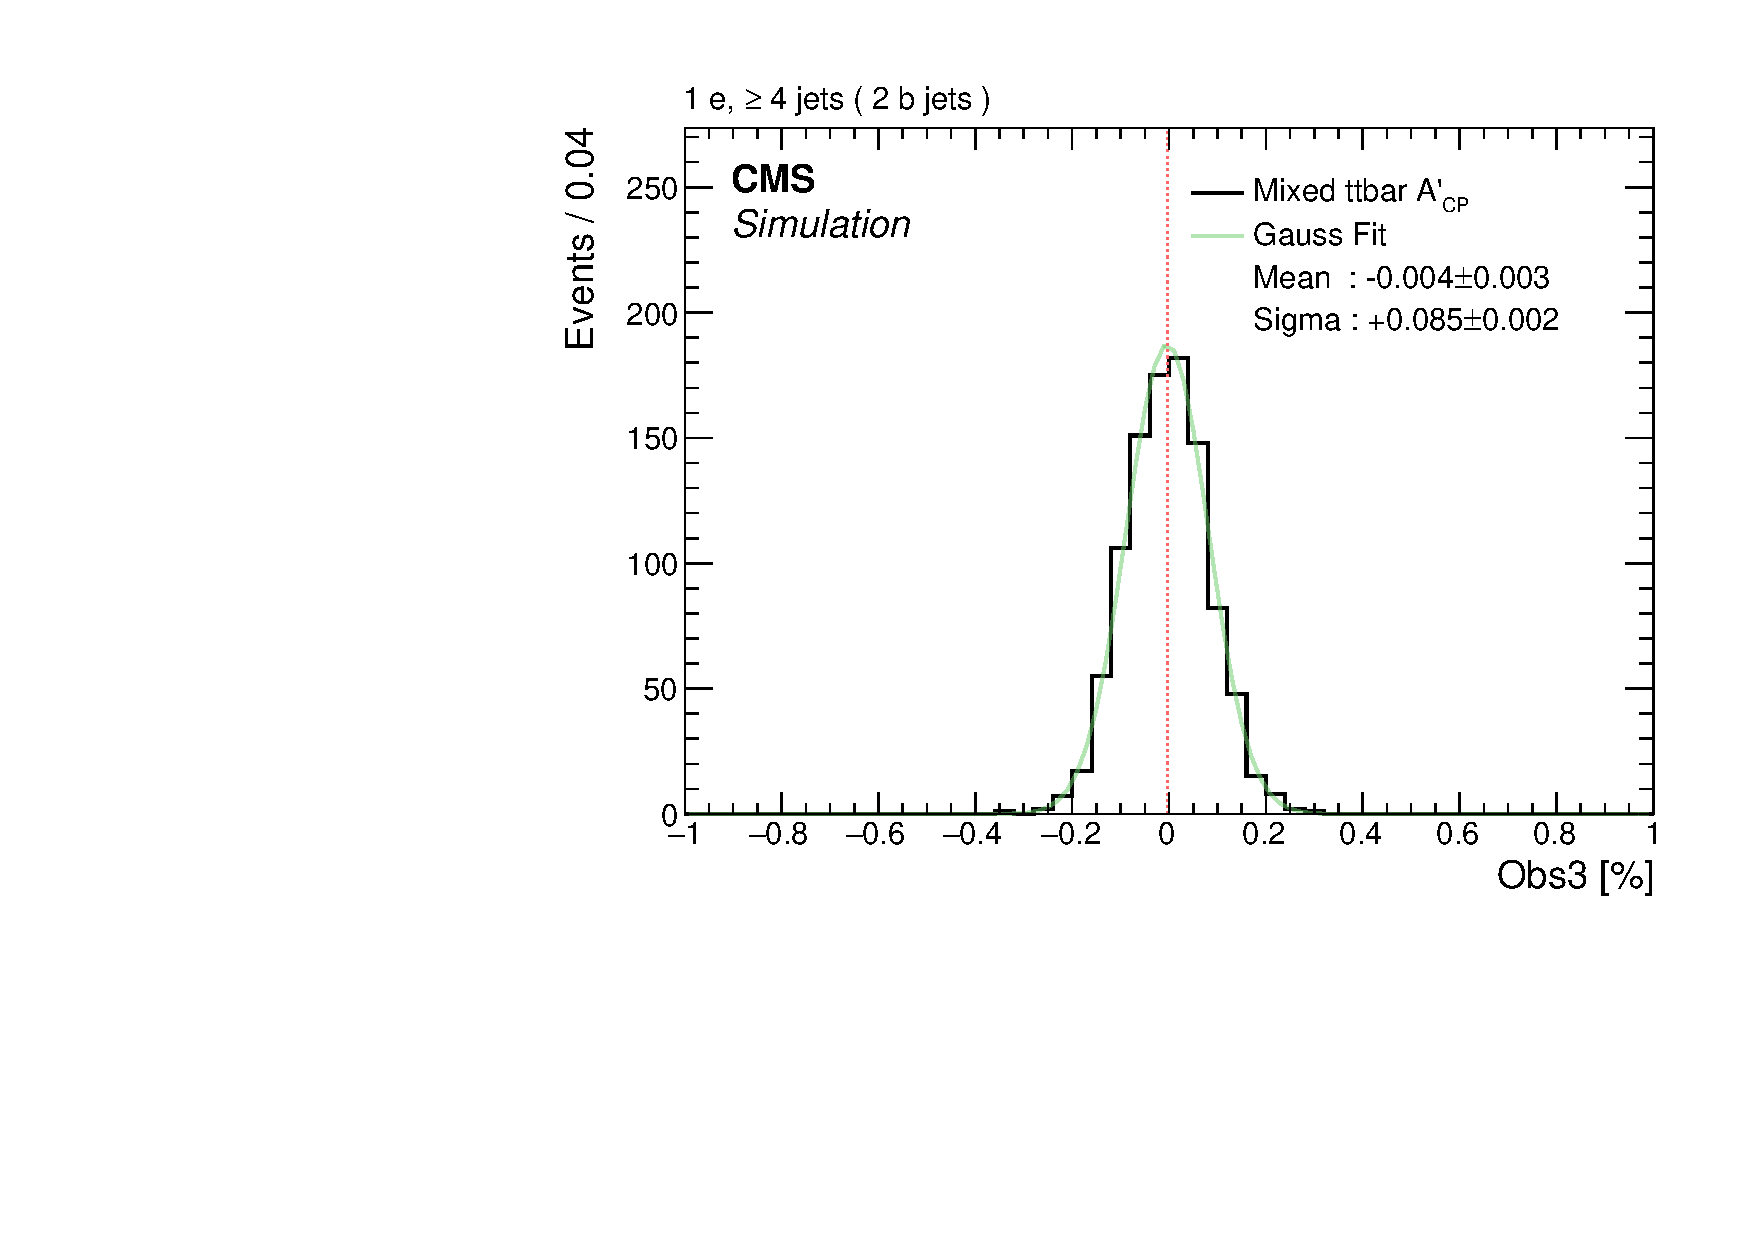
\includegraphics[width=0.45\textwidth]{figure/SimAcp_18_el_Obs3_Acp_10_mixed.pdf}
    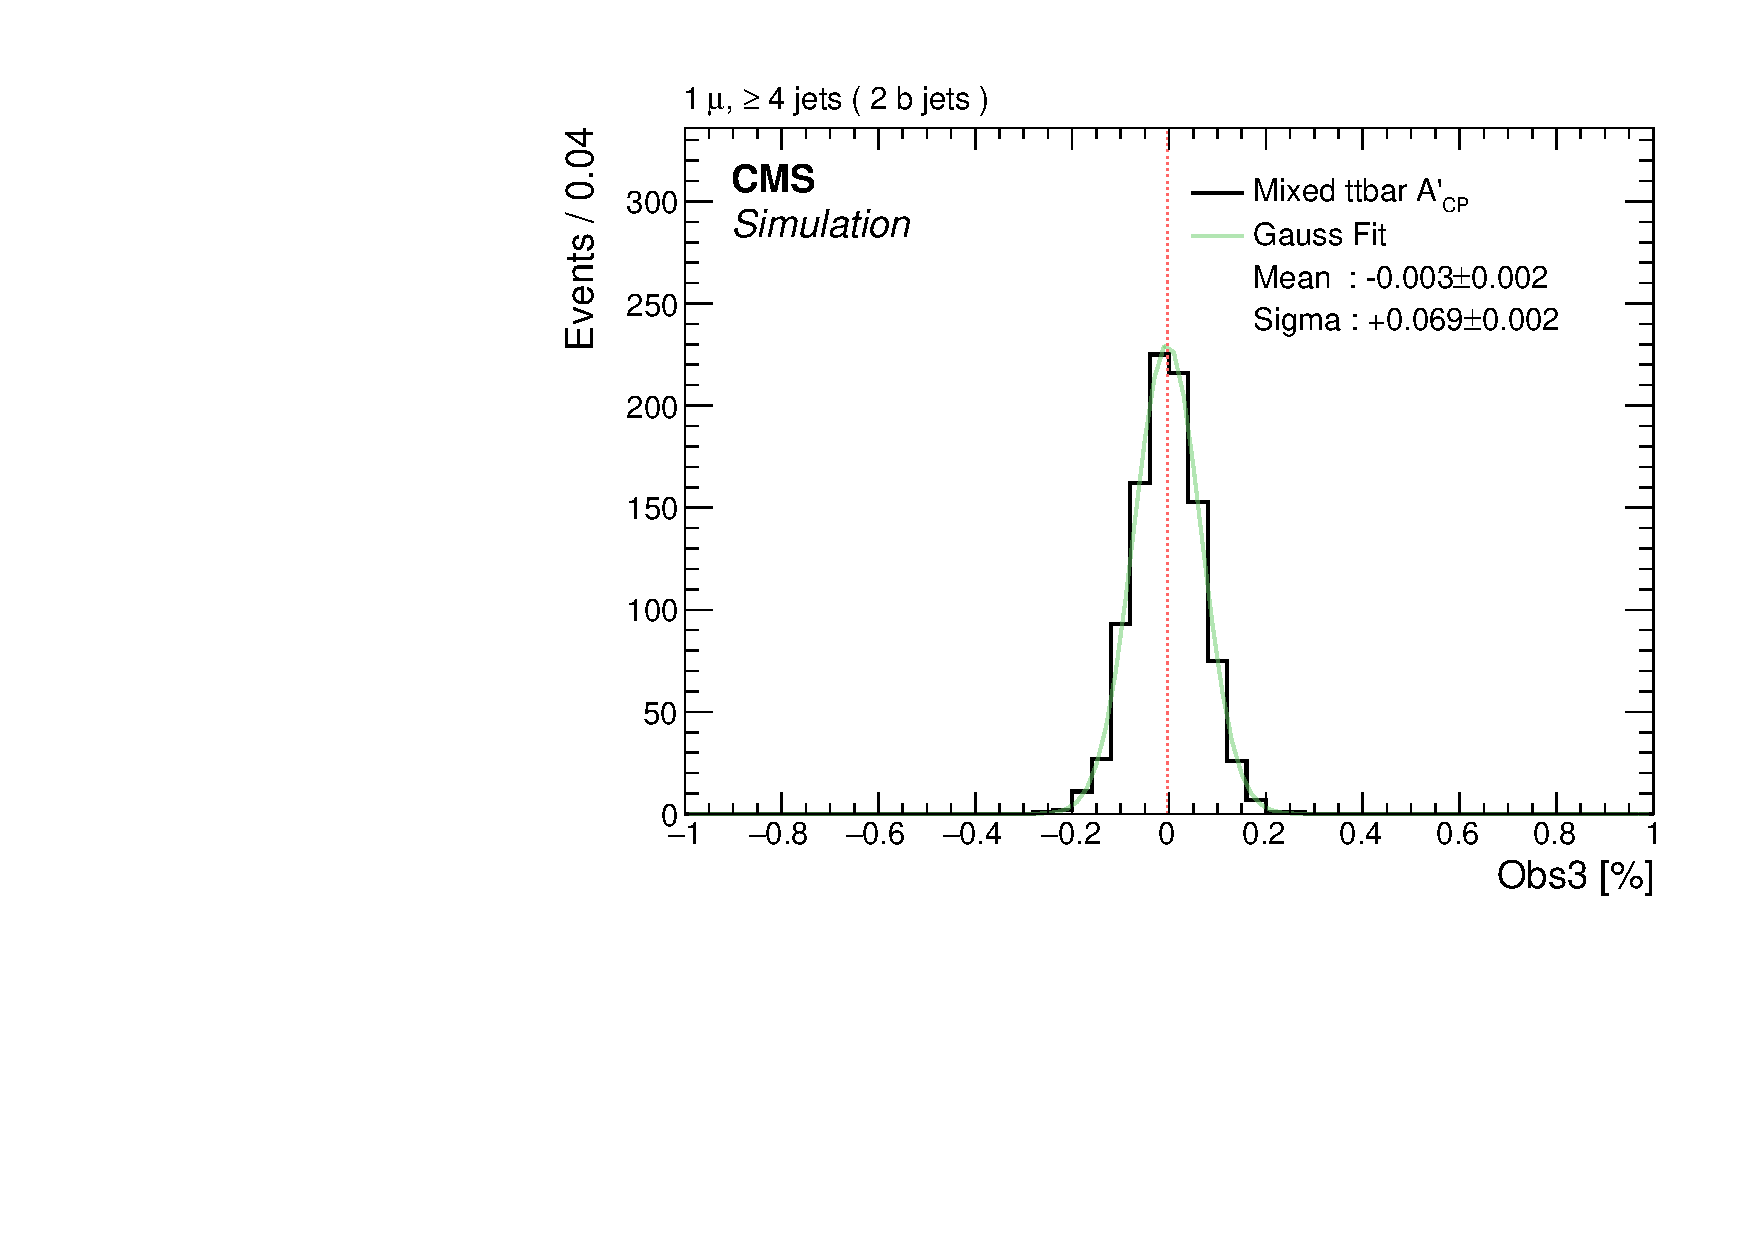
\includegraphics[width=0.45\textwidth]{figure/SimAcp_18_mu_Obs3_Acp_10_mixed.pdf}
    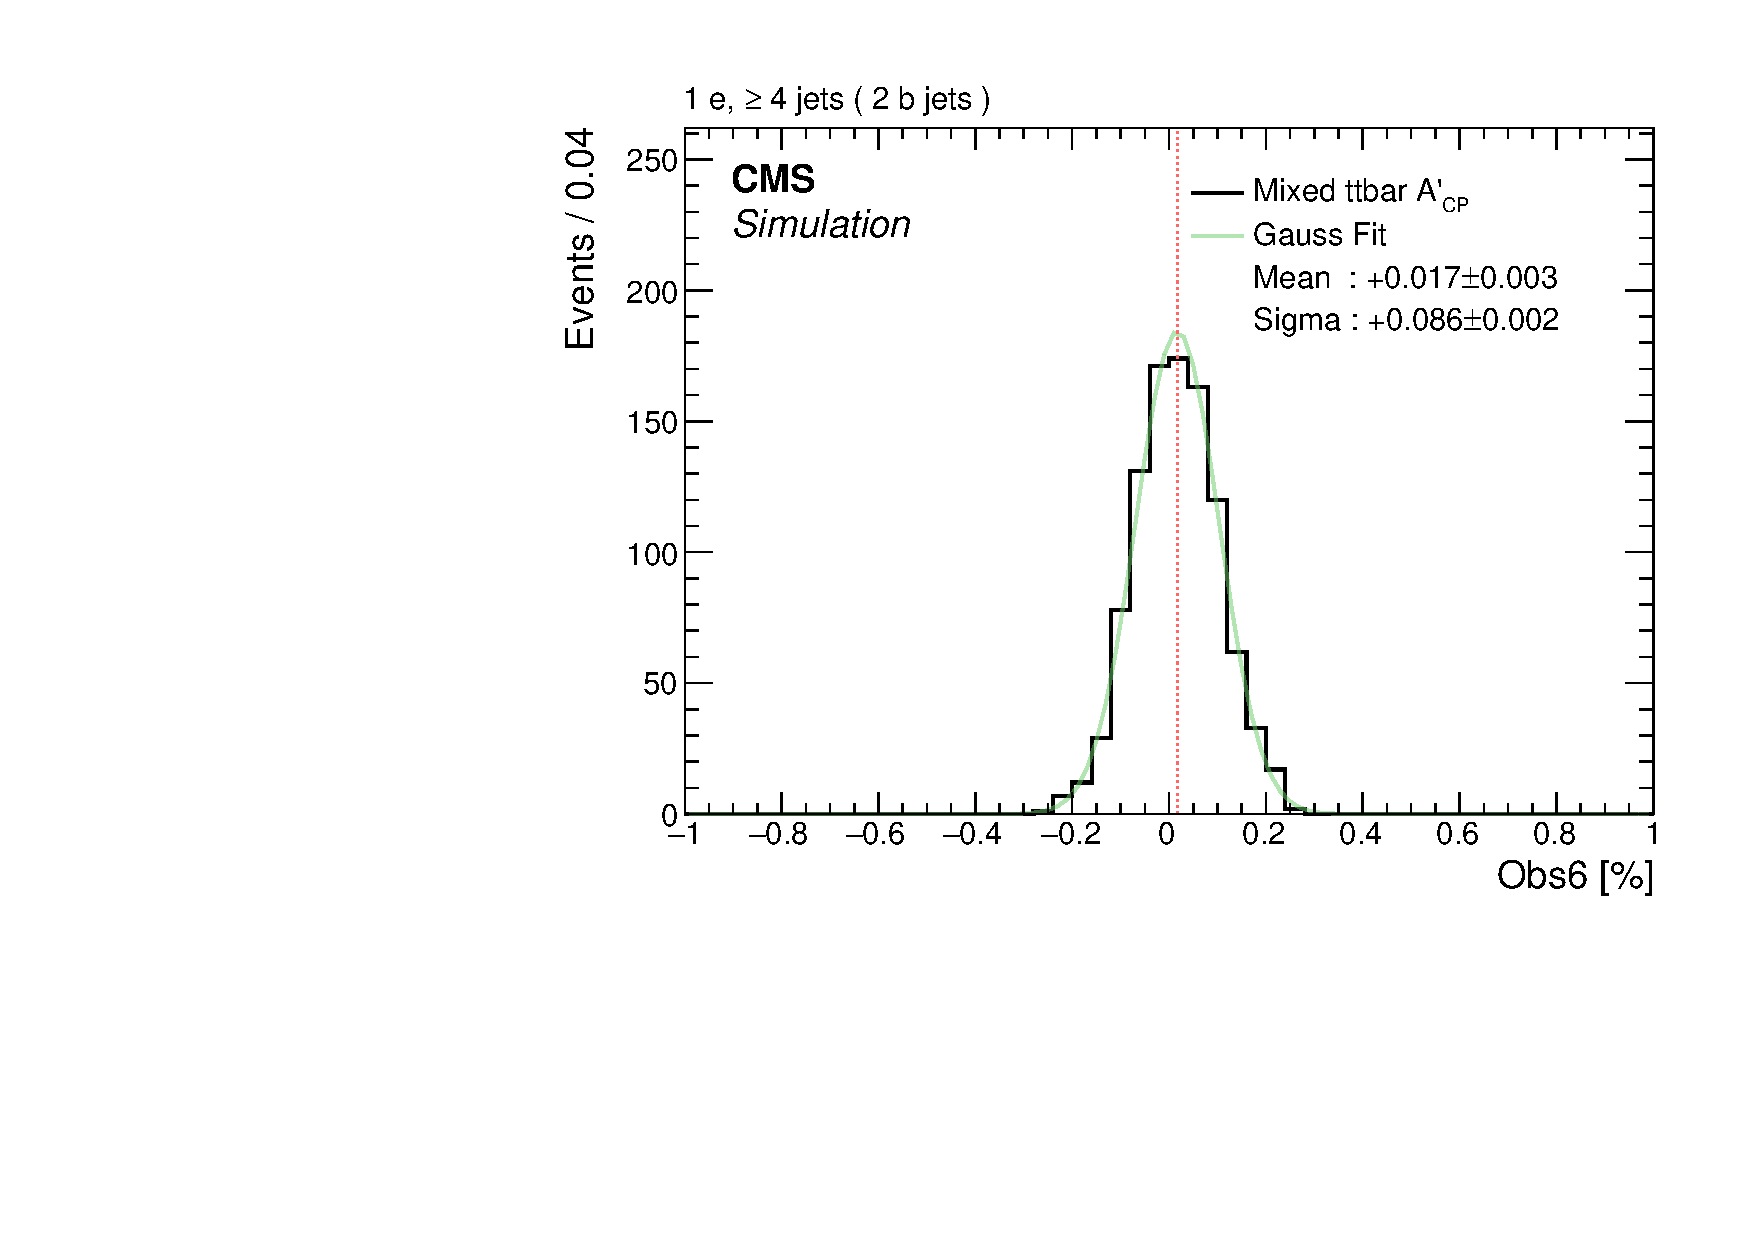
\includegraphics[width=0.45\textwidth]{figure/SimAcp_18_el_Obs6_Acp_10_mixed.pdf}
    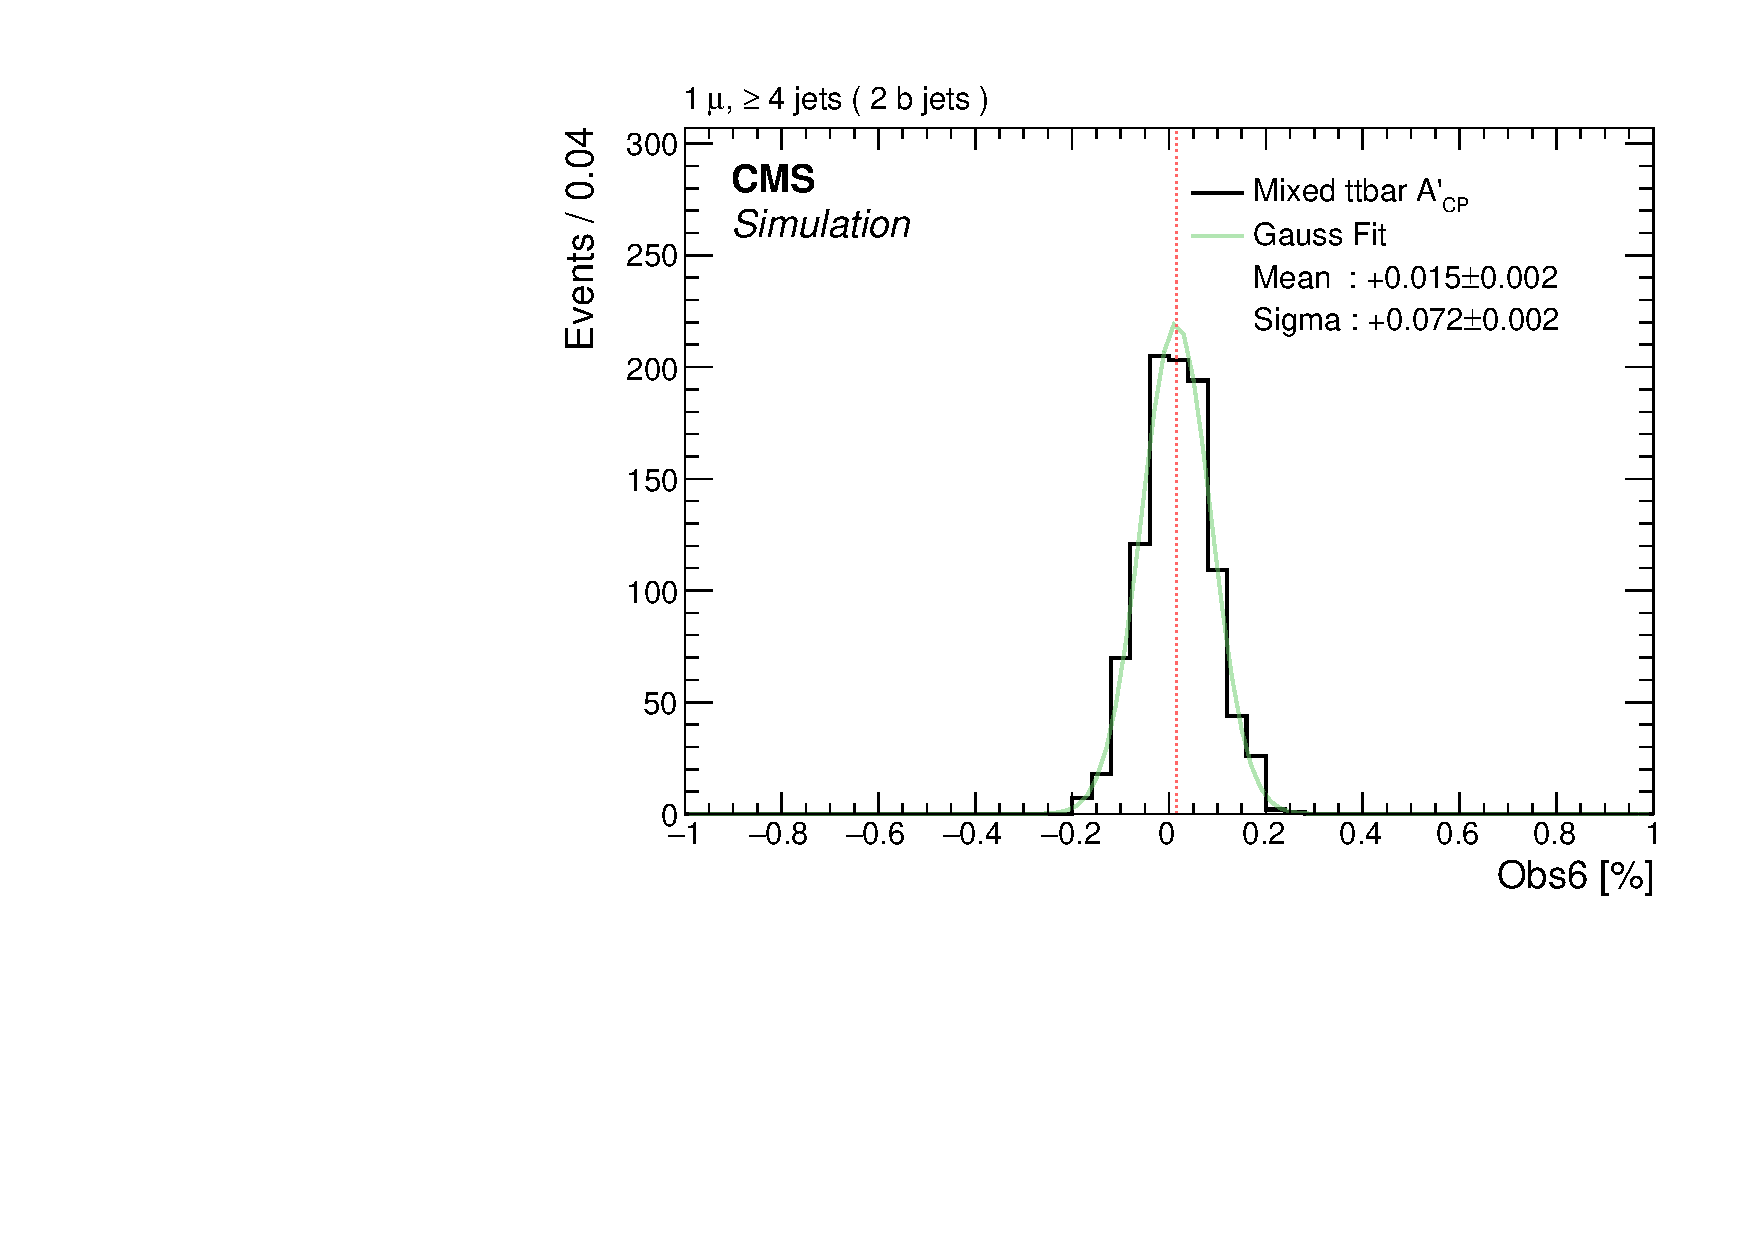
\includegraphics[width=0.45\textwidth]{figure/SimAcp_18_mu_Obs6_Acp_10_mixed.pdf}
    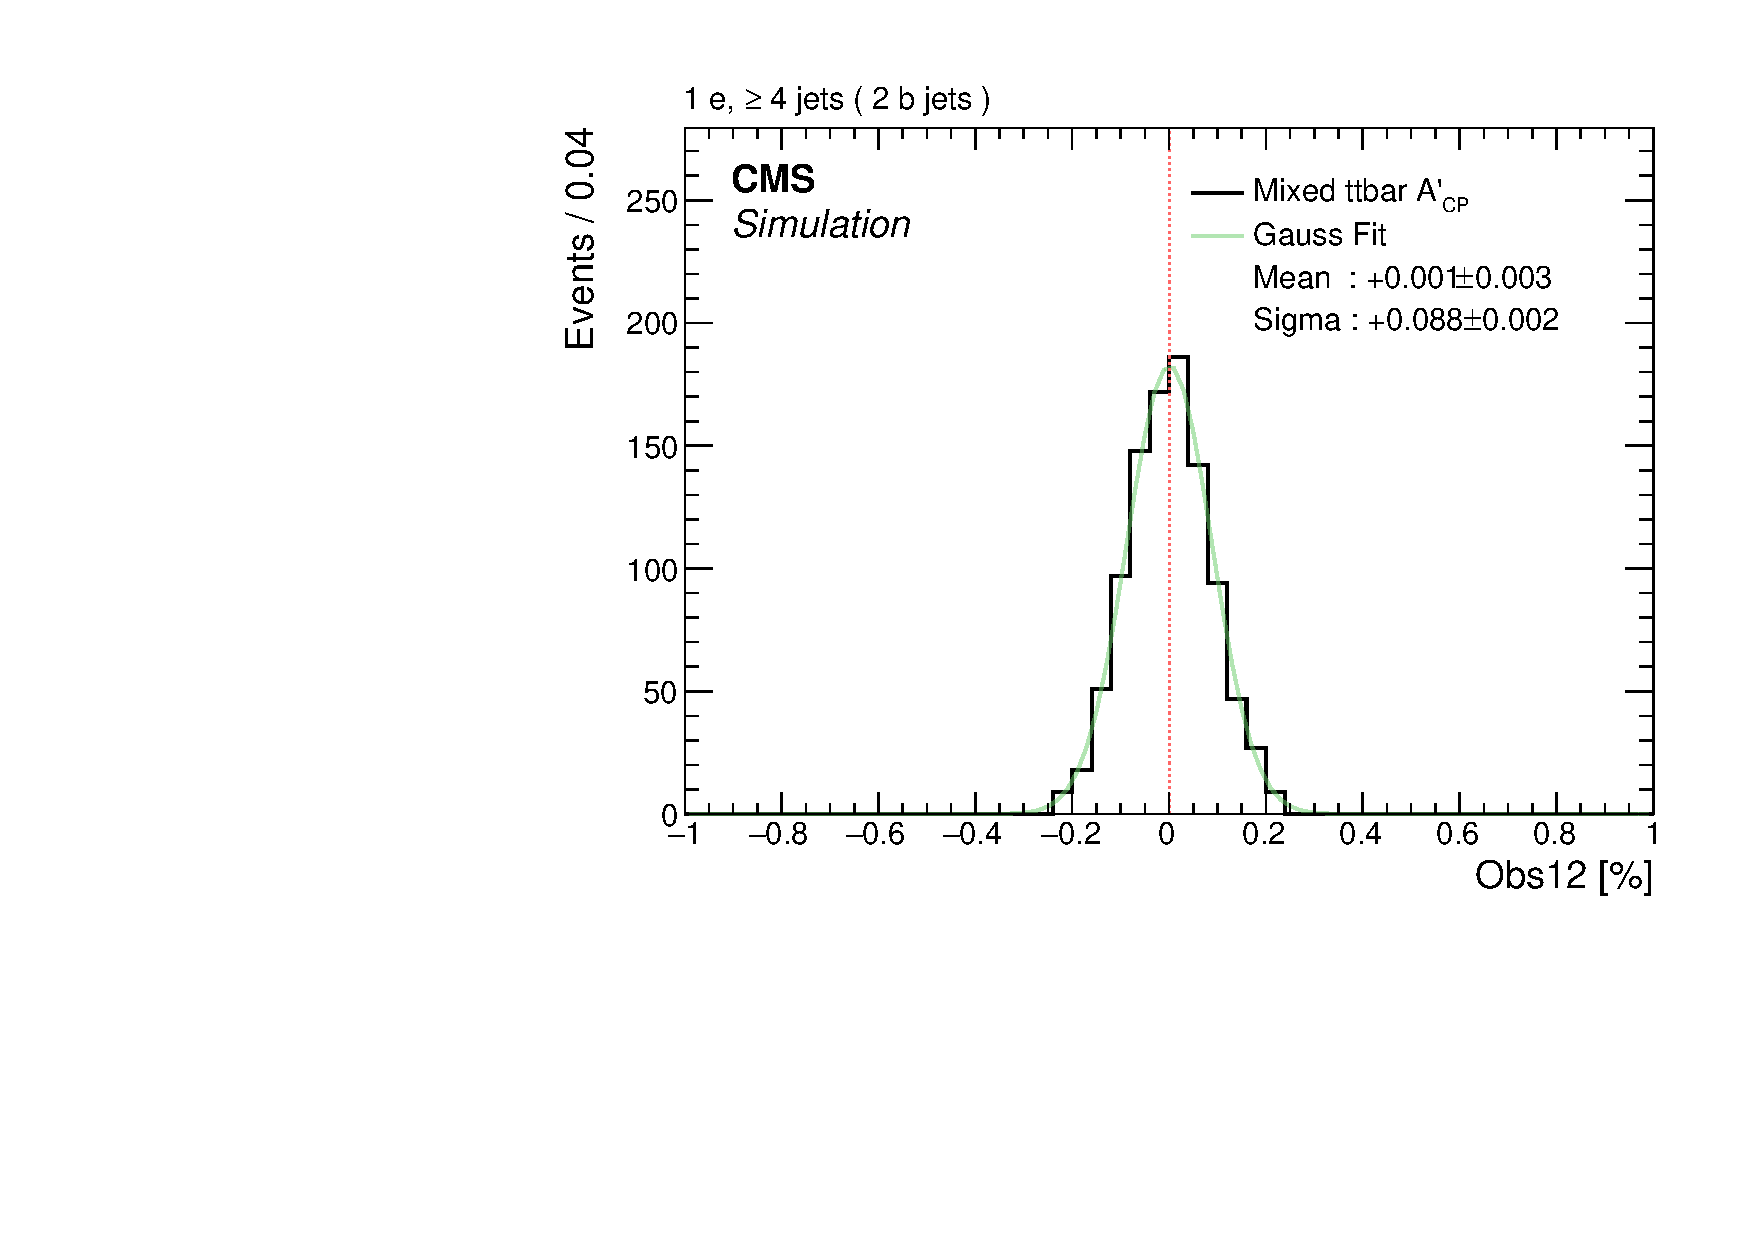
\includegraphics[width=0.45\textwidth]{figure/SimAcp_18_el_Obs12_Acp_10_mixed.pdf}
    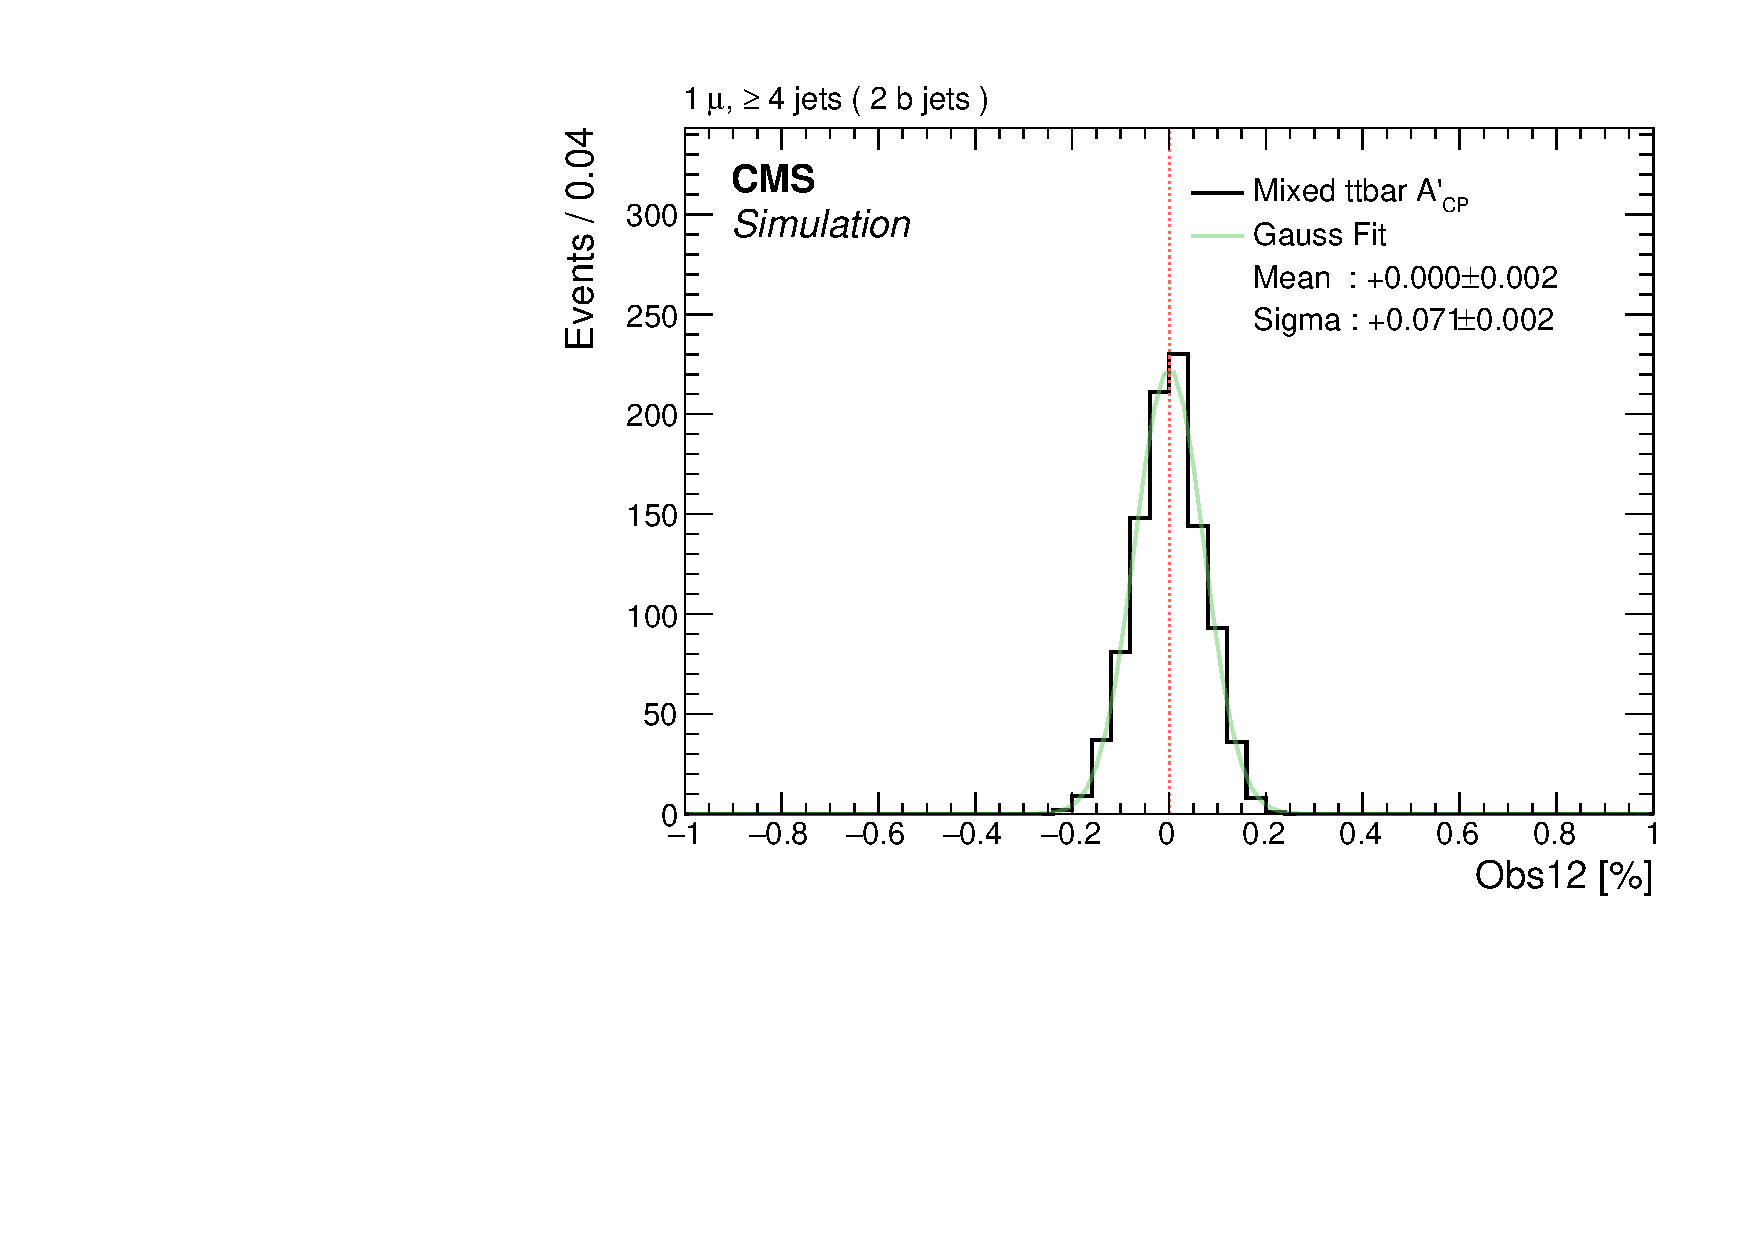
\includegraphics[width=0.45\textwidth]{figure/SimAcp_18_mu_Obs12_Acp_10_mixed.pdf}
    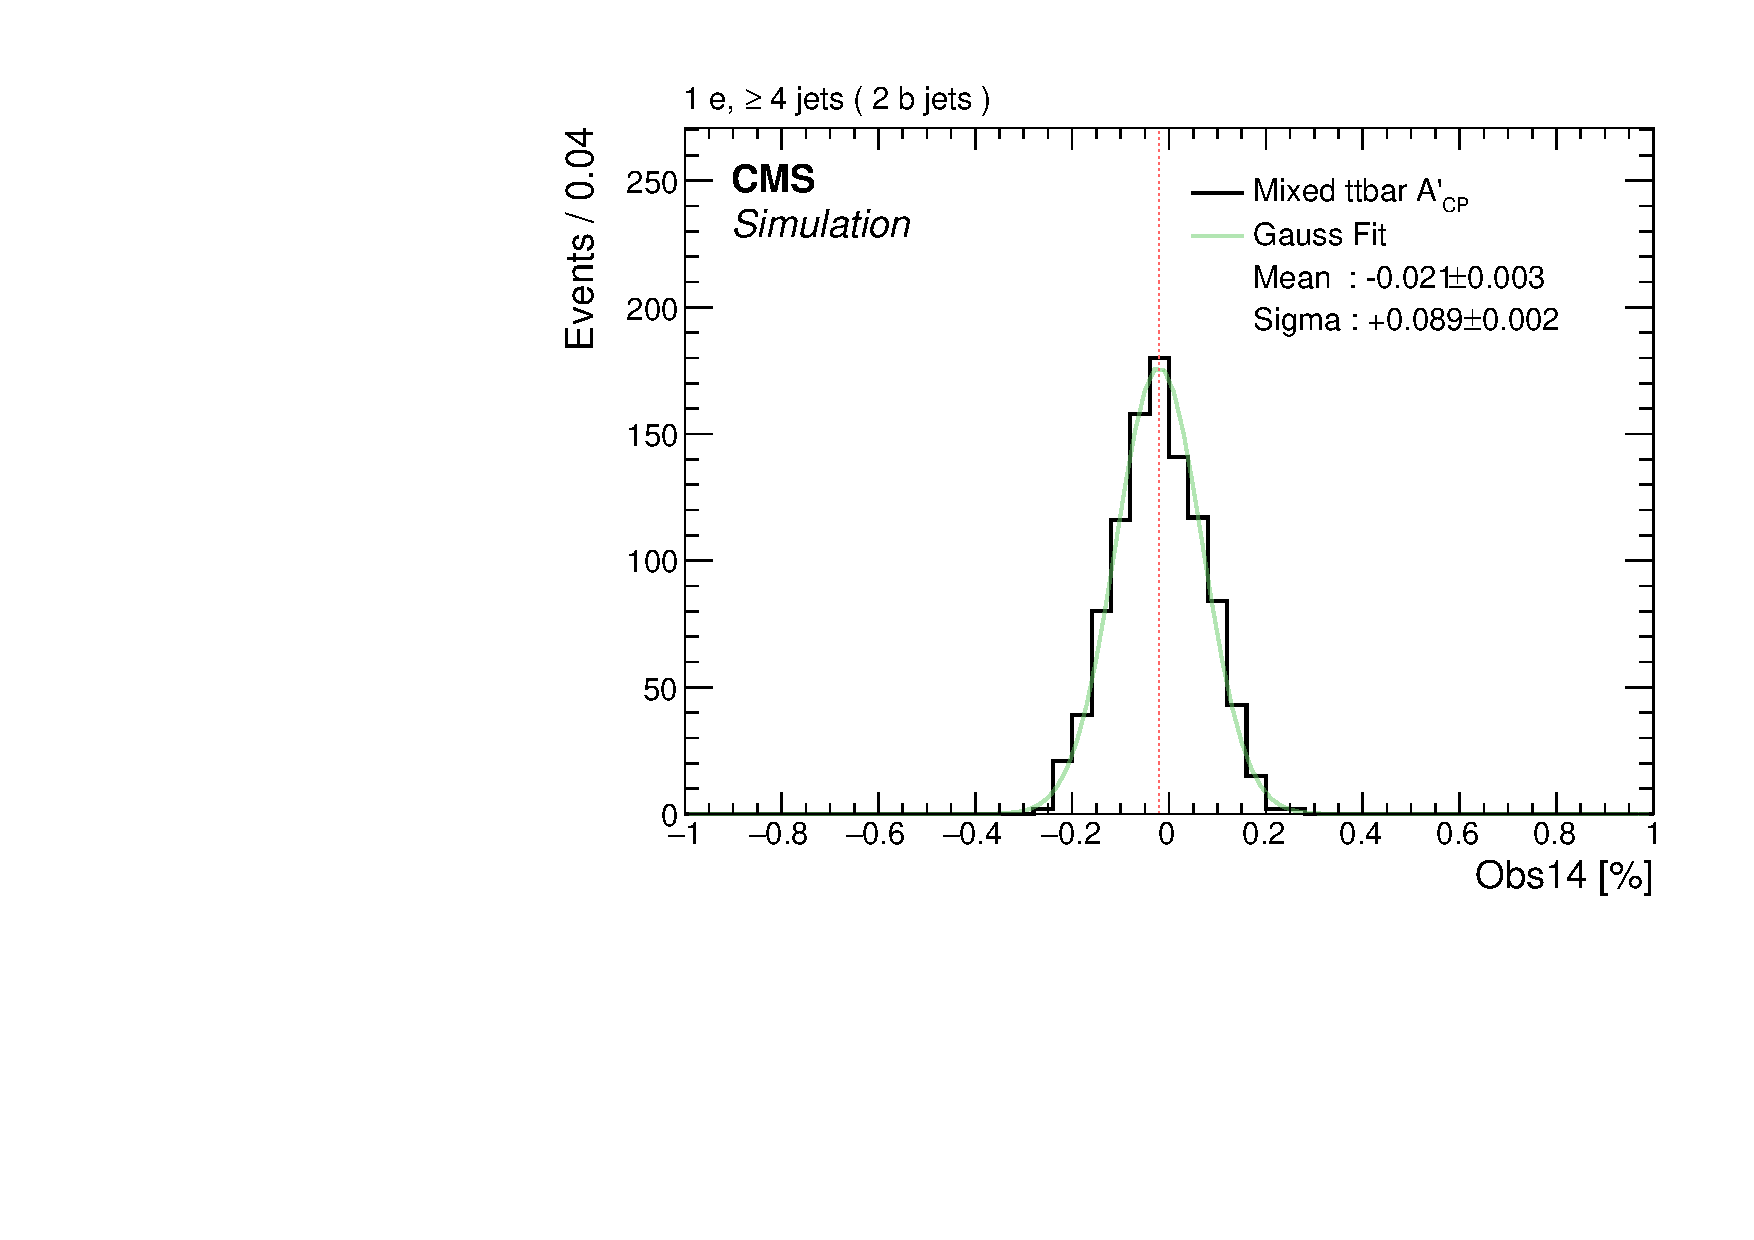
\includegraphics[width=0.45\textwidth]{figure/SimAcp_18_el_Obs14_Acp_10_mixed.pdf}
    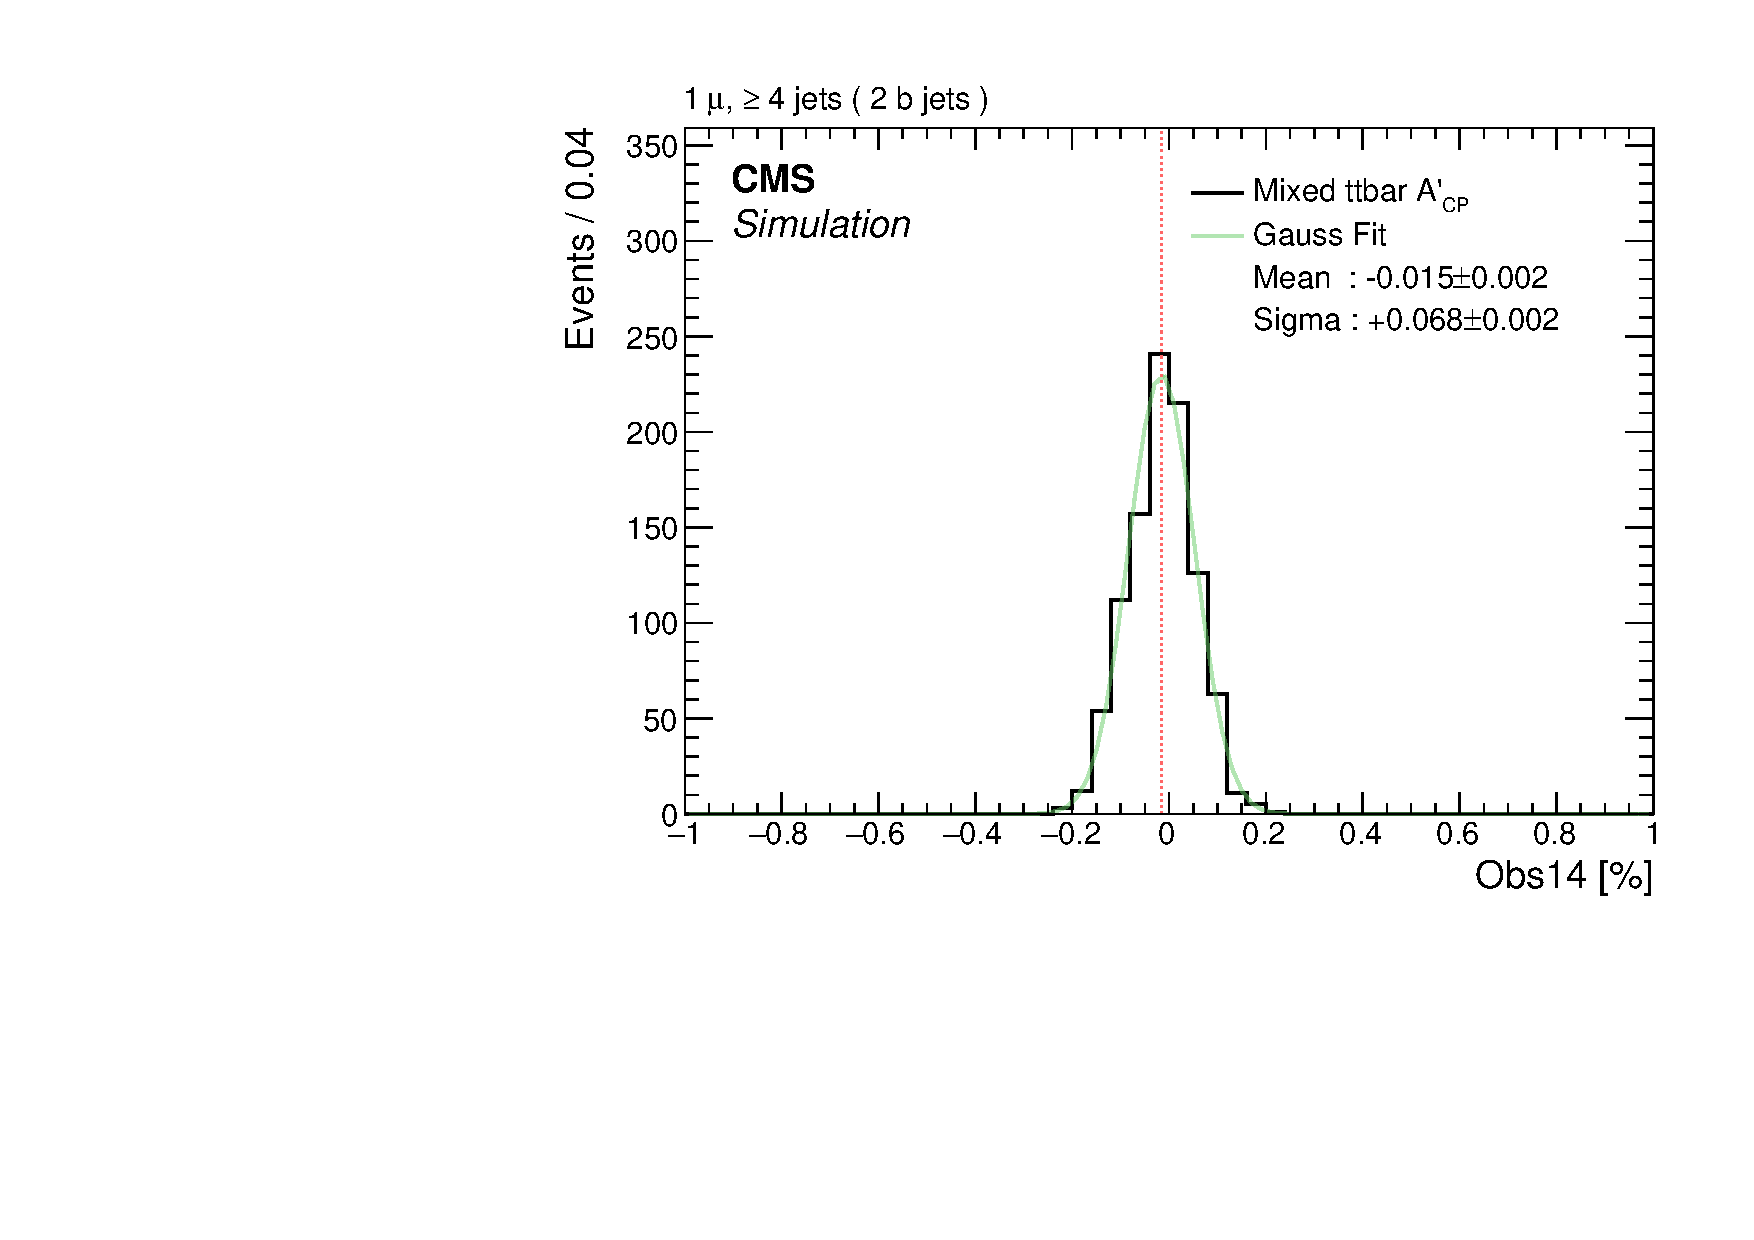
\includegraphics[width=0.45\textwidth]{figure/SimAcp_18_mu_Obs14_Acp_10_mixed.pdf}
    \caption[The \Acpprime distribution after applying the event-mixing method to \ttbar events in 2018 samples.]
    {
        The \Acpprime distribution after applying the event-mixing method to \ttbar events with artificial \Acpprime in 2018 samples. 
        The green line is the fitted gaussian and the red dotted line presents the mean value of the gaussian.
        The electron channel is on the left, and the muon channel is on the right.
    }
    \label{fig:18_exchanging_simulation_acp}
\end{figure}

\begin{figure}

    \centering
    \includegraphics[width=0.45\textwidth]{figure/SimAcp_16_el_ttbar_semi_Obs12_Acp_0_mixed_bias_0.pdf}
    \includegraphics[width=0.45\textwidth]{figure/SimAcp_16_mu_ttbar_semi_Obs12_Acp_0_mixed_bias_0.pdf}
    \includegraphics[width=0.45\textwidth]{figure/SimAcp_17_el_ttbar_semi_Obs12_Acp_0_mixed_bias_0.pdf}
    \includegraphics[width=0.45\textwidth]{figure/SimAcp_17_mu_ttbar_semi_Obs12_Acp_0_mixed_bias_0.pdf}
    \includegraphics[width=0.45\textwidth]{figure/SimAcp_18_el_ttbar_semi_Obs12_Acp_0_mixed_bias_0.pdf}
    \includegraphics[width=0.45\textwidth]{figure/SimAcp_18_mu_ttbar_semi_Obs12_Acp_0_mixed_bias_0.pdf}
    \caption[The $A'_{CP}$ for samples with intrinsic detector bias for each observable.]
    {
        The $A'_{CP}$ for samples with intrinsic detector bias for each observable before and after applying the event-mixing method for both channels.
        The green(yellow) band is the statistical uncertainty with $1\sigma$($2\sigma$) of the standard deviation(s).
        The electron channel is on the left, and the muon channel is on the right.
        Plots are for 2016, 2017 and 2018 from the top to the bottom separately.
    }
    \label{fig:closure_test_acp}
\end{figure}
